
\chapter{Logistika očkování a prioritní skupiny}\label{Logistika_ockovani}

\textit{Ludmila Hamplová, Jakub Weiner}
\vspace{15mm}


%Limity a možnosti matematického modelování versus očekávání veřejnosti a decision-makerů: Role matematického modelování v rámci evidence based policies. Co možné není, co možné je a co je potřeba k tomu, aby to možné bylo. 
\section*{Úvod} %Vakcíny jsou nedostatkovým zbožím a nejstarší skupina obyvatel je ohrožena, je nutné se k problému postavit programově
Očkovací program proti covid-19 se stal jednou z největších logistických akcí v novodobých dějinách České republiky. Nelze na ni nahlížet jen jako na prostou distribuci vakcín od výrobců do očkovacích center, ale jako na komplexní proces řady na sebe navazujících kroků a vyžadující spolupráci mnoha aktérů. Akce tohoto rozměru byla pro stát (i pro svět) v dané době nová a nebylo možné vycházet z předobrazu jiné soudobé logistické operace. Organizace české očkovací kampaně tak proběhla ve značně improvizovaných podmínkách. %Svou roli sehrálo i podcenění rozsáhlosti této akce ze strany státu, který ve srovnání s jinými, zejména evropskými zeměmi začal strategii očkování připravovat až na poslední chvíli a řadu aspektů její operacionalizace řešil až za pochodu, pokud vůbec. To se promítalo i do komunikace státu směrem k veřejnosti. 


    
Názorně to ilustruje skutečnost, že finální strategii očkování představil premiér laické i odborné veřejnosti na svém facebookovém profilu \cite{logoc_caulidi}. 


Vakcinace občanů České republiky začala v prosinci 2020 v návaznosti na doručení prvních zásob vakcíny Comirnaty a postupně se rozšiřovala spolu s rostoucími dodávkami očkovacích látek a také navyšováním kapacit očkovacích míst. %Do poloviny května bylo podáno více než čtyři miliony dávek celkem čtyř různých vakcín a u asi dvou a čtvrt milionu osob bylo dosaženo plné vakcinace. Do začátku července 2021 pak bylo podáno zhruba osm a půl milionu dávek, přičemž u téměř tří a půl milionu českých občanů bylo očkování ukončeno podáním druhé dávky. Očkování v současnosti (červenec 2021) probíhá napříč republikou v rámci nemocnic a zdravotnických zařízení bez ohledu na jejich zřizovatele, ve velkokapacitních očkovacích centrech a v ordinacích některých praktických lékařů. Okrajově jsou využívány další možnosti očkování, například v podobě mobilních očkovacích týmů \cite{mzcr_prehled} . Páteří očkovacího programu v Česku zůstávají očkovací centra, byť jejich další role je předmětem diskuse \cite{logo_jehly}
%
Očkovací dávky byly v počátku běhu vakcinační kampaně extrémně nedostatkovým zbožím. Spolu s mírou rozšíření pandemie v ČR v prvním kvartálu roku 2021 a rizikem úmrtí na covid-19 mezi nejstaršími skupinami obyvatelstva byly vakcíny v době počátku kampaně nástrojem k zajištění promptní ochrany nejohroženějších skupin. %Nelze opomenout též očkování zdravotníků a pracovníků v oblasti sociální péče, krok, který v dané době mířil k pomoci kapacitně velmi vytíženým nemocnicím.% a současně pomáhal řešit situaci v pobytových zařízeních sociální péče, zejména domovech pro seniory.

Při ohlédnutí za téměř půlročním během očkování lze identifikovat řadu okolností, které může být užitečné vzít při organizaci dalších akcí podobného rozměru v ČR či v zahraničí v potaz. Naprostým základem by mělo být podrobné plánování v dostatečném časovém předstihu za spolupráce řady klíčových hráčů jak na straně vlastní organizace očkovacího programu, tak jeho medicínských i komunikačních aspektů. 
%
Cílem tohoto článku je zhodnotit plnění strategických záměrů očkovací kampaně. To je provedeno za pomoci rekapitulace původního záměru a jeho změn (sekce \ref{sec:strategie}), definicí teoreticky optimálního přístupu k realizaci kampaně (sekce \ref{sec_vypocet}), jeho porovnání s empirickými daty (sekce \ref{sec:comparison}), shrnutím vybraných odchylek a nastíněním důležitých otázek připravenosti pro případné další operace podobného rázu (závěrečná sekce).
%
Článek se (v návaznosti například na \cite{lastmile}) tematicky omezuje na logistiku poslední míle, v jejímž rámci nás zajímá zejména otázka ideálního přístupu k doručení vakcín klíčovým skupinám obyvatel.

%Cílem tohoto článku je zhodnotit, jak efektivně kampaň probíhala, jak se její praktické provedení lišilo od původně definovaných teoretických předpokladů, a také poukázat na možné sporné aspekty. To bude provedeno za pomoci definice teoretického optima (sekce \ref{sec_vypocet}), jeho porování s reálnými daty (kapitola \ref{sec:comparison}), shrnutím silných/slabých míst (kapitola \ref{sec:implikace}) a nastíněním důležitých otázek připravenosti pro případné další operace podobného rázu.




% Ve druhé kapitole jsou představeny teoretické přístupy, s jejichž pomocí lze očkovací kampaň plánovat. Důraz je kladen na nakládání s očkovacími dávkami a plánování prioritních skupin. Úvaha je provedena na analytické úrovni státu, ale je do určité míry přenositelná i na nižší útvary.
%Třetí sekce užívá zjednodušenou verzi představeného přístupu, kterou dává do kontextu s empirickými daty z České republiky. 
%%
%Očkování není čistě jen logistickým (matematickým) problémem, ale vzhledem k množství lidí zapojených v roli organizátorů (stát, kraje, očkovací místa, lékaři) či subjektů (očkovaných, potenciálně očkovaných) má i důležitou behaviorální rovinu. Role očekávání, vůle k naočkování se a různých incentiv je zohledněna v závěrečné (diskusní) kapitole.

\section*{Strategické záměry a realizace očkovací kampaně v ČR}
\label{sec:strategie}

Ve Strategii očkování \cite{strategie_covid} je definován cíl co nejrychlejšího proočkování skupin ohrožených těžkým průběhem nemoci, respektive úmrtím, což také odpovídá doporučením Světové zdravotnické organizace (WHO) a Evropského střediska pro prevenci a kontrolu nemocí (ECDC). Postup prioritizace jednotlivých skupin obyvatelstva a operační aspekty jsou podrobně definovány v Metodickém pokynu \cite{ockovani_mp}. %Rozbor jednotlivých aspektů původního záměru, praktické realizace a míry přiblížení se možnému je poskytnut v rámci jednotlivých bloků této sekce textu. Důraz je kladen postupně na prioritizaci, logistiku očkování a práci s informacemi.
%

MZ ČR ve Strategii vychází ze statisticky identifikované silné závislosti úmrtnosti na covid-19 a věku, respektive vážných onemocnění (komorbidit). Prioritizační přístup tak předpokládá dvě klíčové skupiny, kde do první (I.A, plán očkování v lednu-únoru 2021) byly umístěny osoby nad 80 let věku, osoby v institucionalizované péči (například v pobytových zařízeních pro seniory) včetně ošetřovatelského a zdravotnického personálu v rámci klíčových oborů potřebných pro boj s pandemií. Skupina I.A byla posléze rozšířena o zaměstnance orgánů ochrany veřejného zdraví \cite{prioritizace_hygiena}. 

%
Druhou uvažovanou prioritní skupinou je I.B (plán očkování únor-březen/duben 2021), do níž byly zahrnuty osoby nad 60 let věku, pracovníci kritické infrastruktury, chronicky nemocní splňující předem definované podmínky závažnosti svého stavu a pedagogičtí pracovníci. %Prakticky však byla definice kritické infrastruktury státu definována velmi široce.
Pedagogickým pracovníkům byla následně uvnitř skupiny zvýšena priorita, čímž se dostali do úvodní části skupiny \cite{prioritizace_ockovani}. Zbytek dospělé populace (očkovaný mimo prioritizaci dle vlastního zájmu) byl jako skupina II. naplánován od března/dubna 2021 do konce očkovací kampaně. Vládní Covid Portál uvádí, že cílová proočkovanost skupin I.A a I.B je 70 procent s tím, že pro obě skupiny jí nemusí být dosaženo v případě nedostatečného zájmu \cite{kdoprvni}.

%\subsection*{Reálný průběh a aktuální stav očkovací kampaně}
Celkem bylo k 16. 5. 2021 (posuzovanému datu) podáno 4 147 719 očkovacích dávek, přičemž u 1 106 784 osob bylo ukončeno očkování podáním jednodávkové vakcíny nebo druhé dávky dvoudávkové vakcíny \cite{mzcr_data}. Grafy přiložené k článku ukazují různé pohledy na uvažované množství, konkrétně efektivity nakládání se zásobami, stavu distribuční sítě a dělení dávek do prioritních skupin.



\begin{table}
\begin{minipage}{\textwidth} 
%\begin{adjustbox}{width=1\textwidth}
\begin{centering}
\begin{tabular}{|c|c|c|c|c|}
\hline
& \textbf{Osob} & \textbf{Cíl} & \textbf{\% (Ukončeno)} & \textbf{\% (jen 1. dávka)}  \\
\hline
\textbf{I.A} & 778,237 & 70\% & 67\% & 21\% \\
\hline
\textbf{I.B} & 3,727,731 & 70\% & 12\% & 30\%\\
\hline
\textbf{II.} & 3,493,657 & - & 4\% & 19\% \\
\hline
\end{tabular}
%\end{adjustbox}
	\caption{Přehled prioritních skupin, jejich cílové proočkovanosti dle Strategie a stavu k 16. 5. 2021 \cite{strategie_covid}. Počet osob ve skupině II. je dopočítán jako doplněk do dospělé populace ČR dle dat Českého statistického úřadu \cite{obyvatele_pocet}.}
    \label{tab_skupiny}
    
    \end{centering}
\end{minipage}
\end{table}


%Dělení dávek do prioritních skupin
Na grafu \ref{gr_proockovanost} je vidět stav proočkovanosti jednotlivých skupin k 16. 5. 2021. Z vývoje je patrné, že v rámci nejkritičtější skupiny I.A mají k danému datu významný náskok zdravotničtí pracovníci včetně nelékařských profesí, kteří jsou ke sledovanému datu 1. dávkou proočkováni na úroveň 105 \%\footnote{Toto zjištění se může na první pohled jevit jako nesmyslné. Ve skutečnosti však poukazuje na okolnost v rámci výkaznictví, kdy byl původní odhad o velikosti skupiny nepřesný či jsou do něj nyní započítáváni i zdravotníci mimo úvodní prioritizaci, respektive v rámci očkovací kampaně byli očkováni i zaměstnanci zdravotnických zařízení, kteří nespadají mezi zdravotnické pracovníky definované podle 96/2004 Sb. Zákon o nelékařských zdravotnických povoláních.} a dokončení očkování na úroveň 82 \%. Prioritizovaní dle zdravotního stavu\footnote{Do této skupiny je zahrnut i pečovatelský personál v institucionalizované péči, jenž není v rámci dat MZ ČR evidenčně odlišen od pacientů.} dosahují 82 \% pro první dávku a očkování je ukončeno u 60 \% z nich. Další skupiny následují. 
%
Graf \ref{gr_skupiny_davky} zobrazuje celkově doručené dávky v jednotlivých měsících minulého a tohoto roku a jejich využití jednotlivými skupinami. Z hlediska využitelnosti dávek je vidět, že v lednu a únoru 2021 se očkovalo agregátně méně, než by množství doručených očkovacích dávek umožňovalo. V březnu byl přebytek z předcházejících měsíců doháněn, v dubnu však nebylo aplikováno ani doručené množství vakcín. Dále je (dohromady i se stavem proočkovanosti z grafu \ref{gr_proockovanost}) patrné, že očkování skupiny I.B v souladu s představeným plánem bylo zahájeno od března 2021, ale skupina I.A nebyla dle původního plánu ke konci února doočkována.
%
Na prioritizaci lze nahlížet i z hlediska věku, tento pohled je zahrnut v rámci grafu \ref{gr_skupiny_davky_vek}.


%Práce se zásobami
Na grafu \ref{gr_vyuziti} je vidět ve větším detailu využití dávek dostupných ve skladu. Z grafu je patrné, že podíl uskladněných dávek (částečně čekajících na využití pro druhé očkování dvoudávkovou vakcínou či vyhozených na konci očkovacího dne) se přibližně do přelomu února a března držel stabilně nad 25 \% a od dané doby klesá.
%
Graf \ref{gr_vyuziti_zrizovatele} zobrazuje podíl provedených vakcinací dle zřizovatelů očkovacích center.

%Poskytovatelé




\begin{figure}
\centering

\begin{subfigure}{0.9\textwidth}
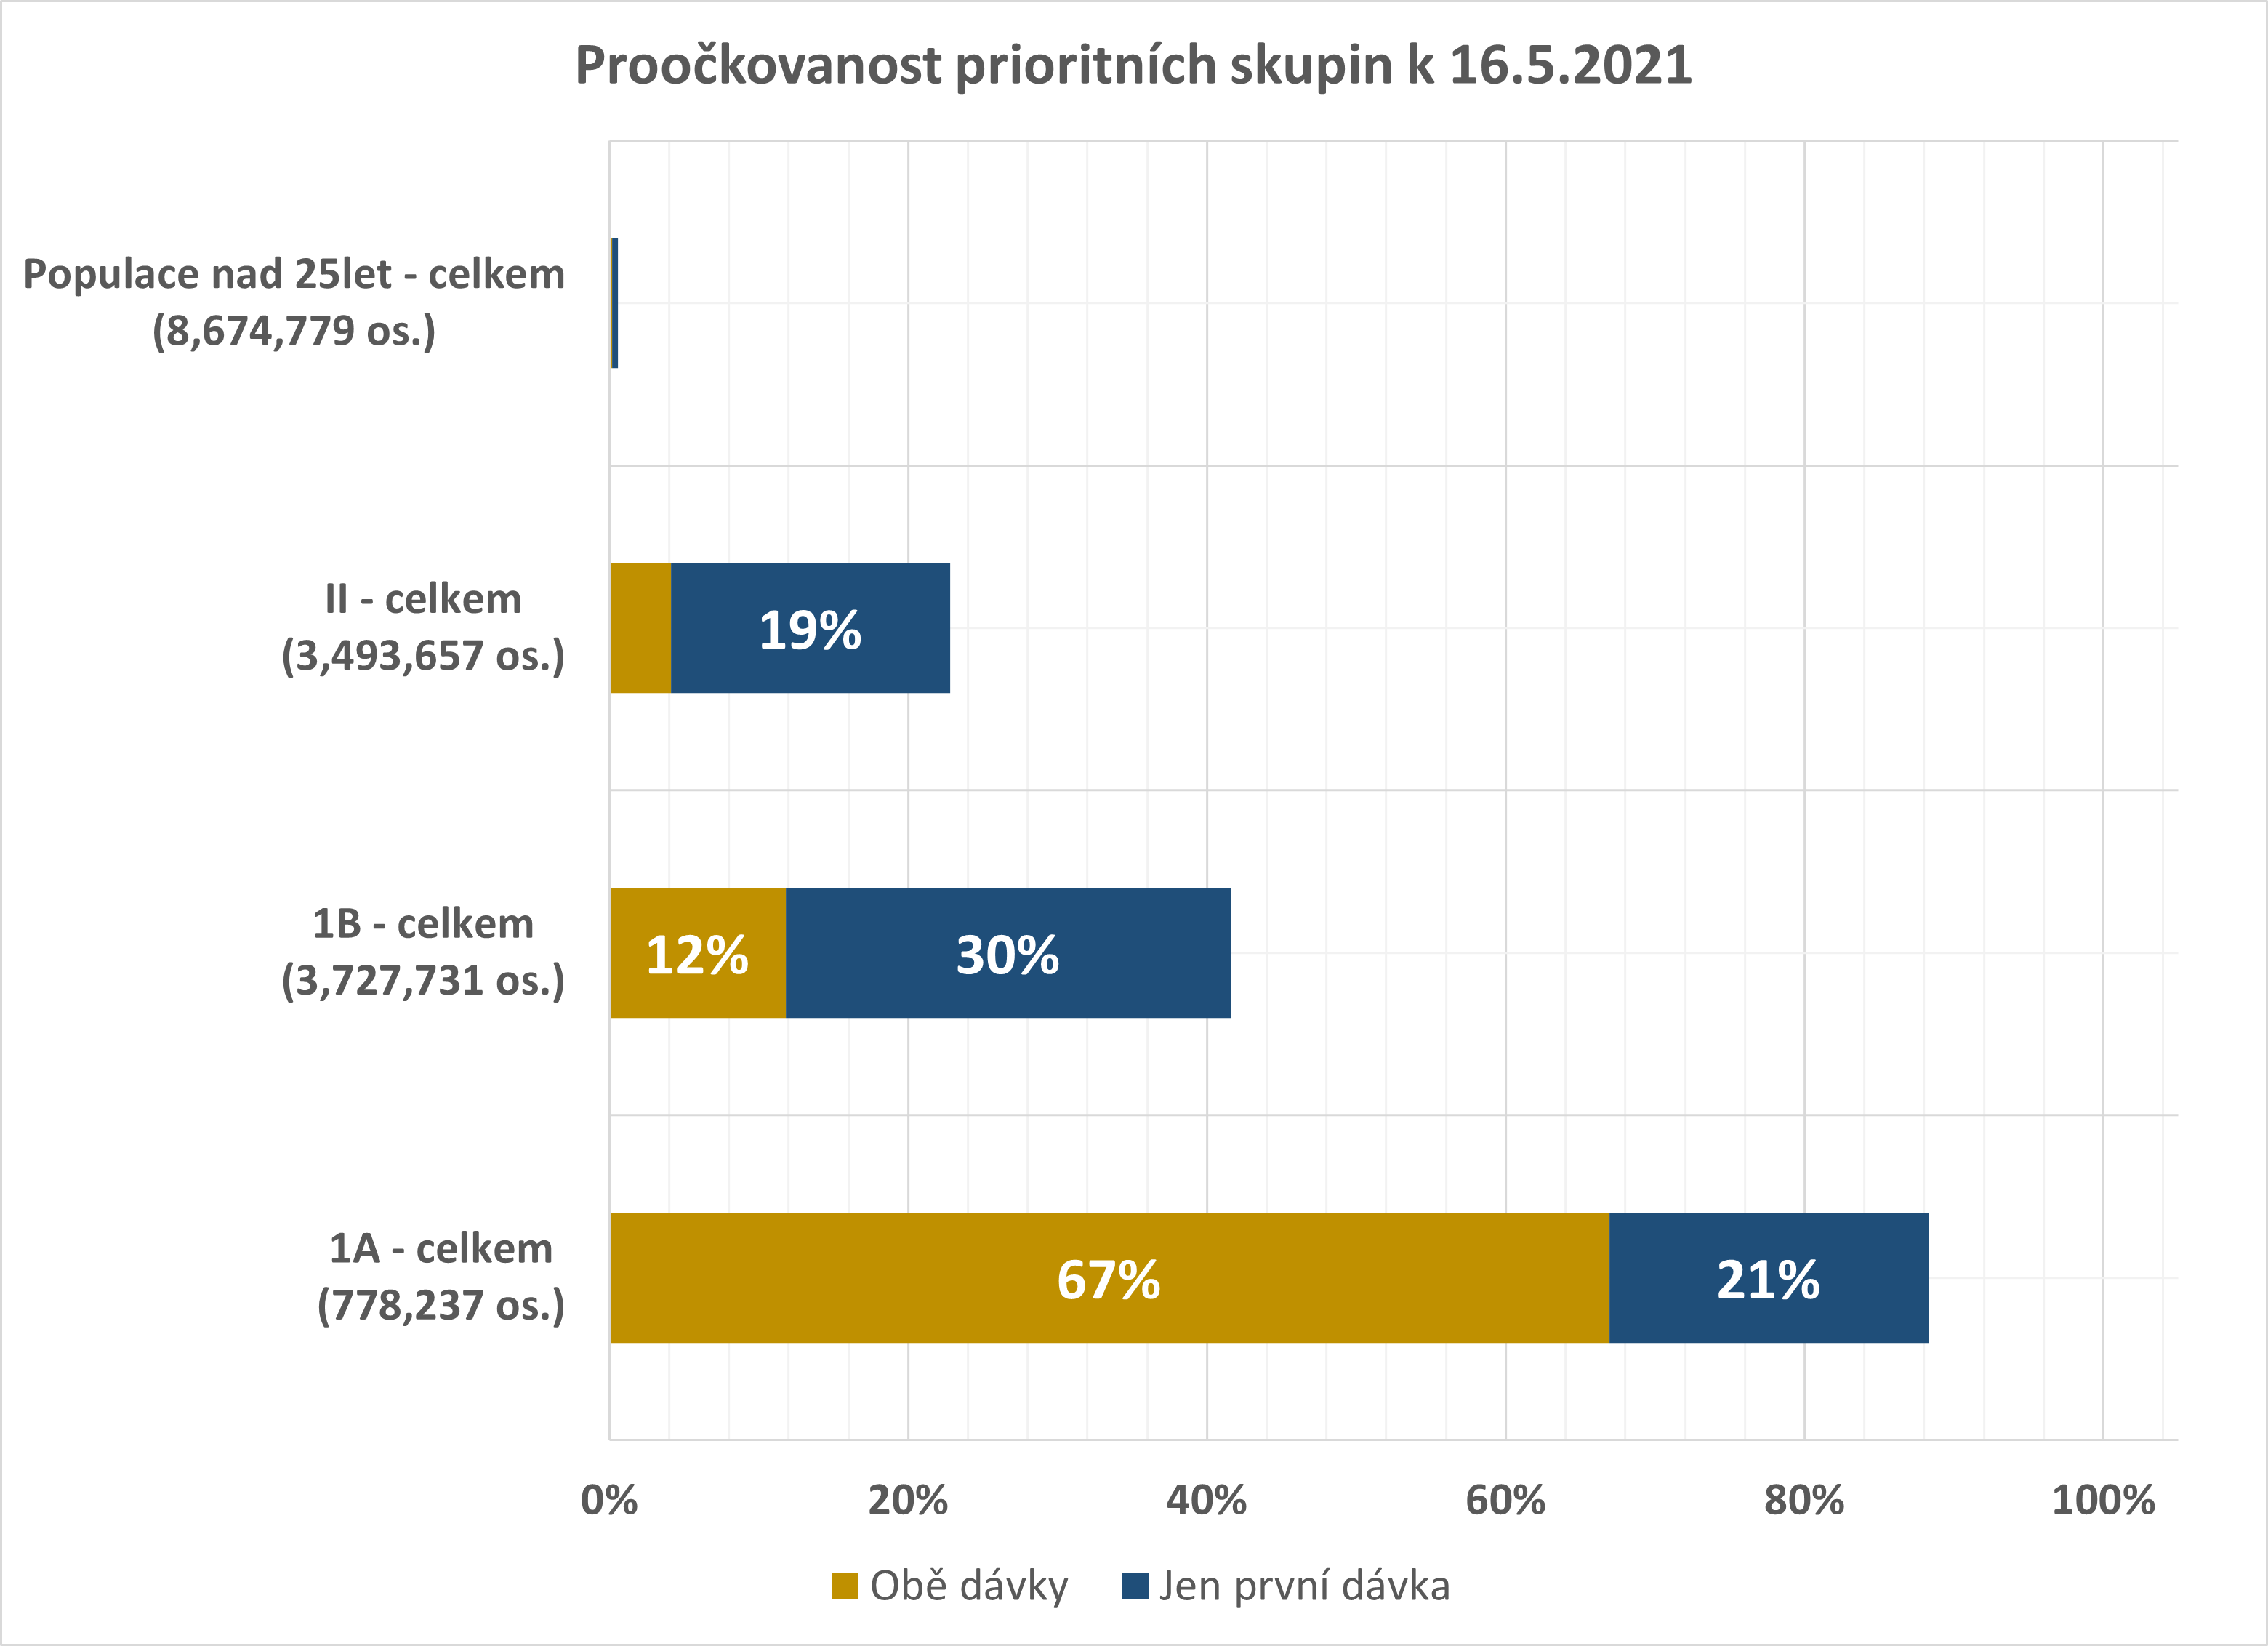
\includegraphics[height=0.3\textheight, width=\textwidth]{assets/proockovanost_vsechnyPS}
\caption{Všechny prioritní skupiny}
\label{proockovanost_ps_vsechny}
\end{subfigure}

\begin{subfigure}{0.9\textwidth}
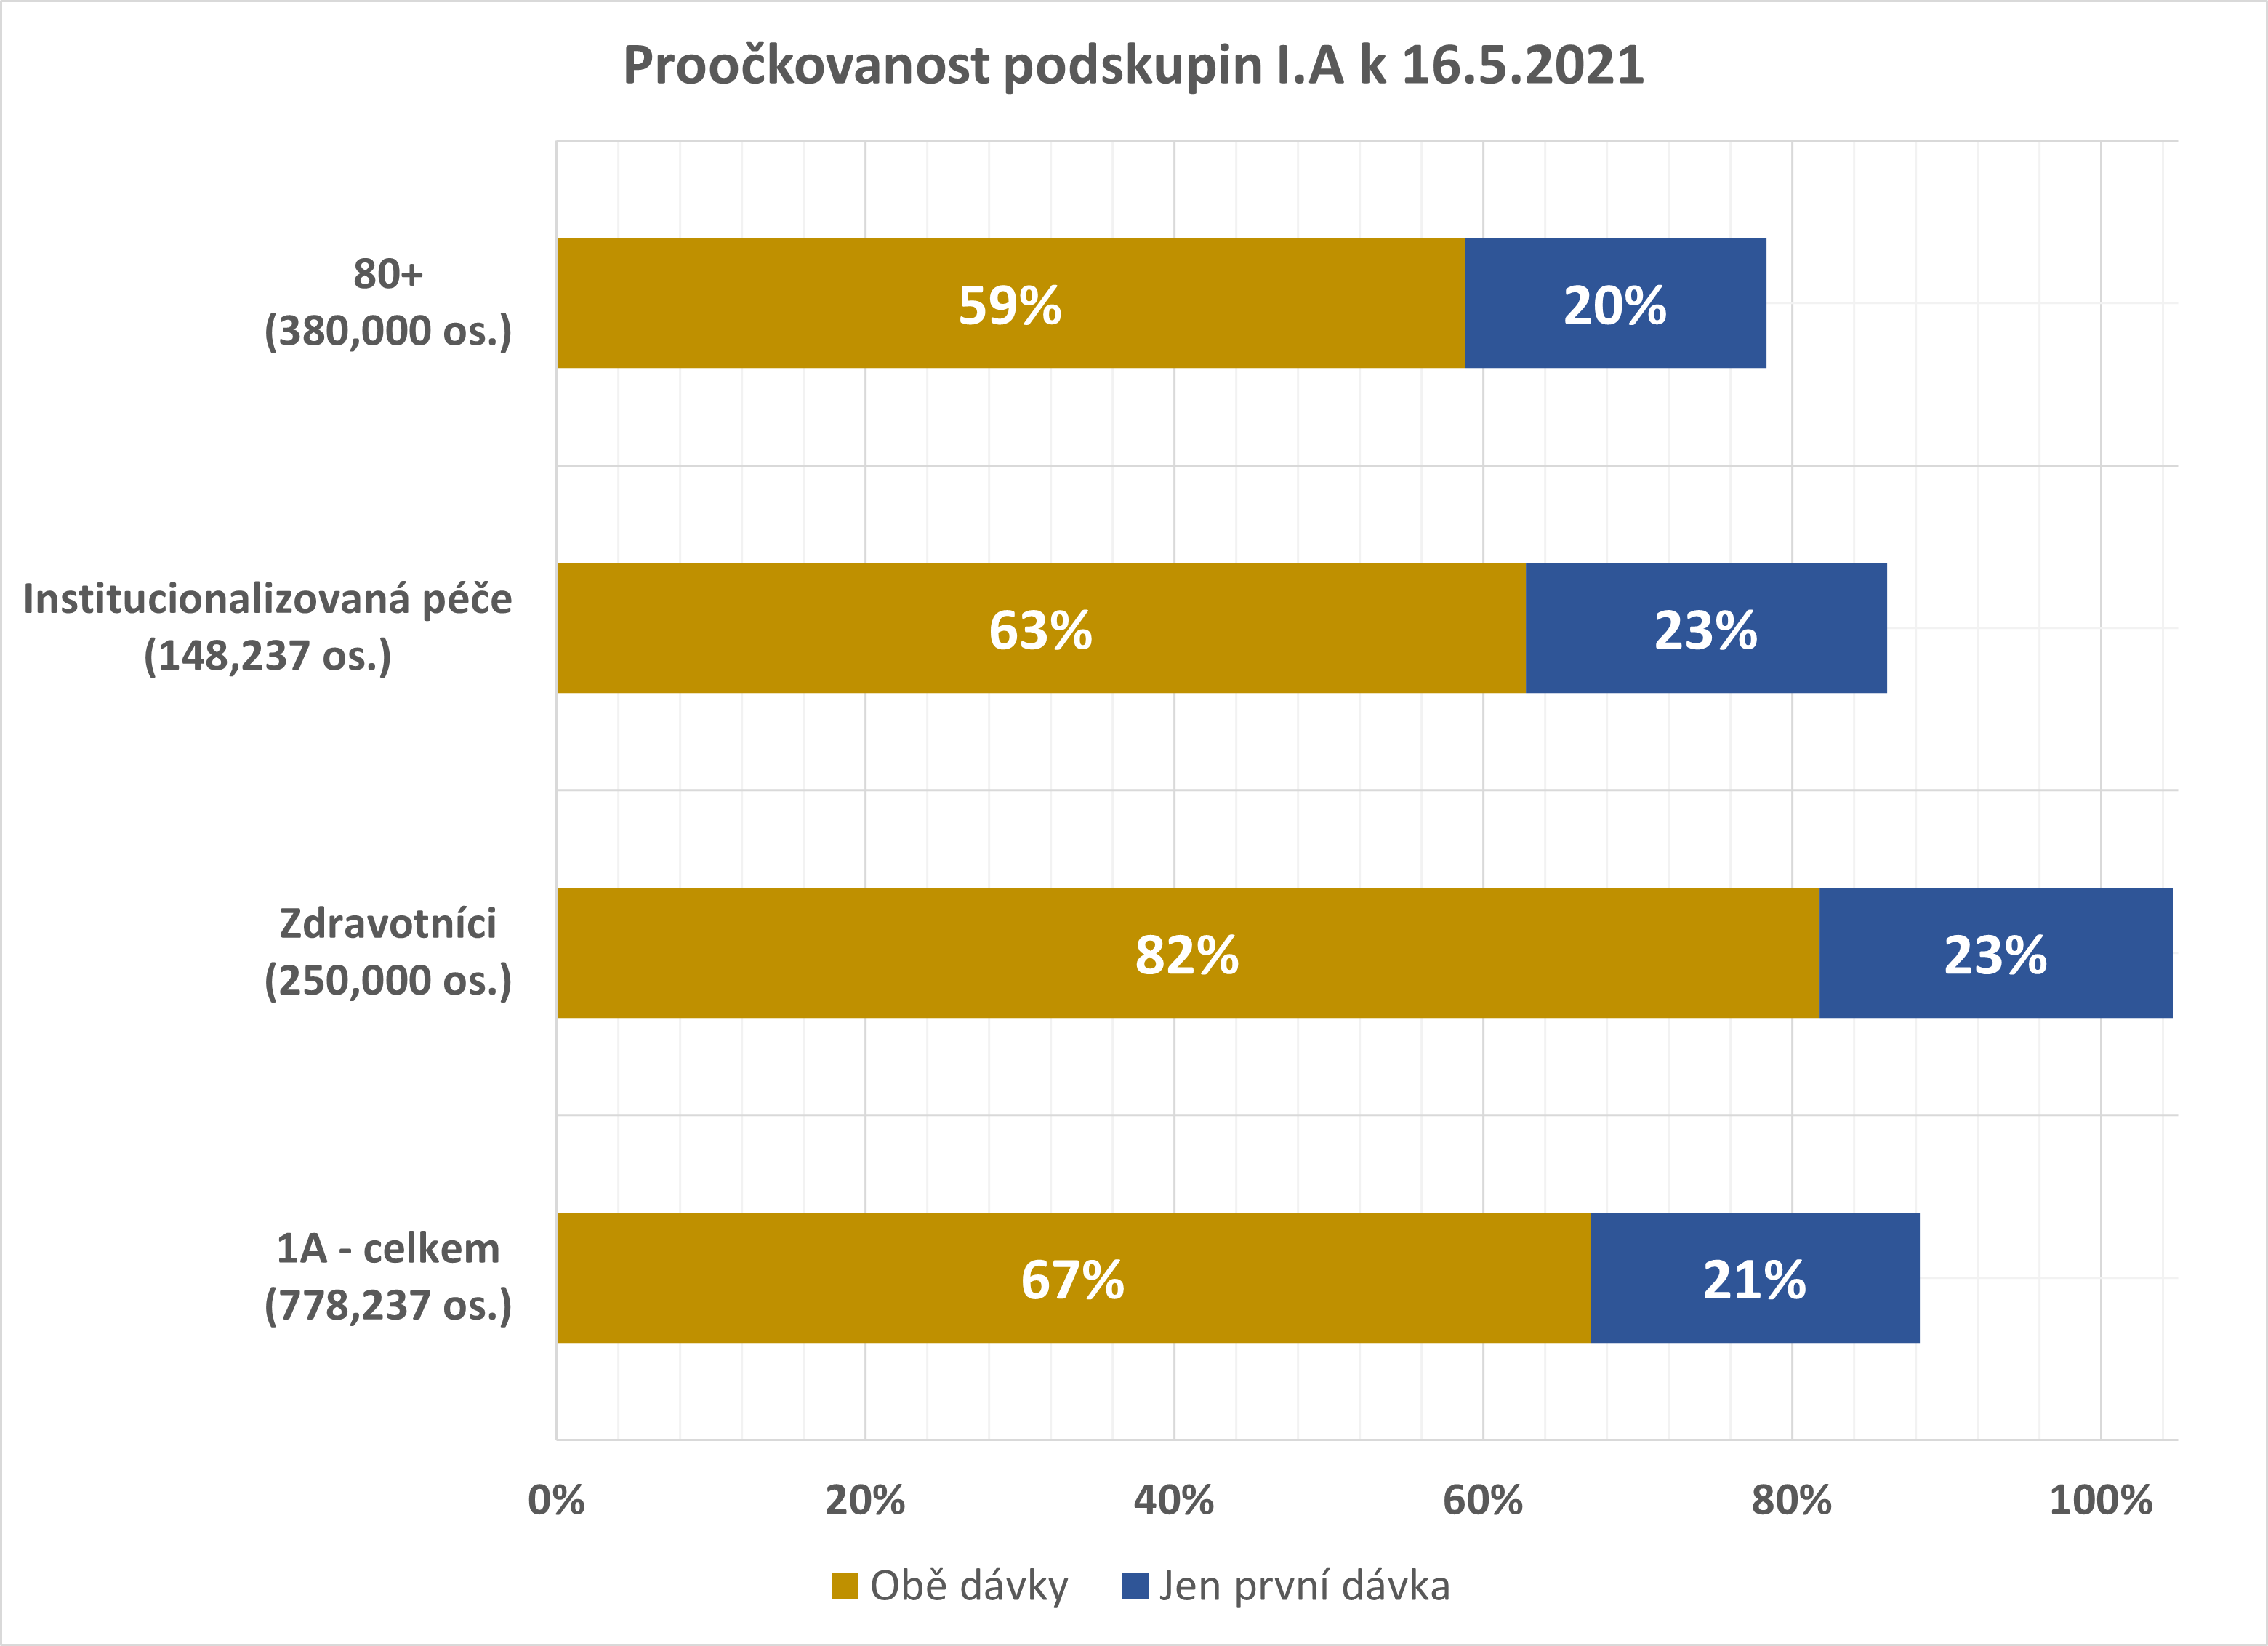
\includegraphics[height=0.3\textheight, width=\textwidth]{assets/proockovanost_1A}
\caption{Podskupiny v rámci I.A}
\label{proockovanost_ps_1a}
\end{subfigure}

\begin{subfigure}{0.9\textwidth}
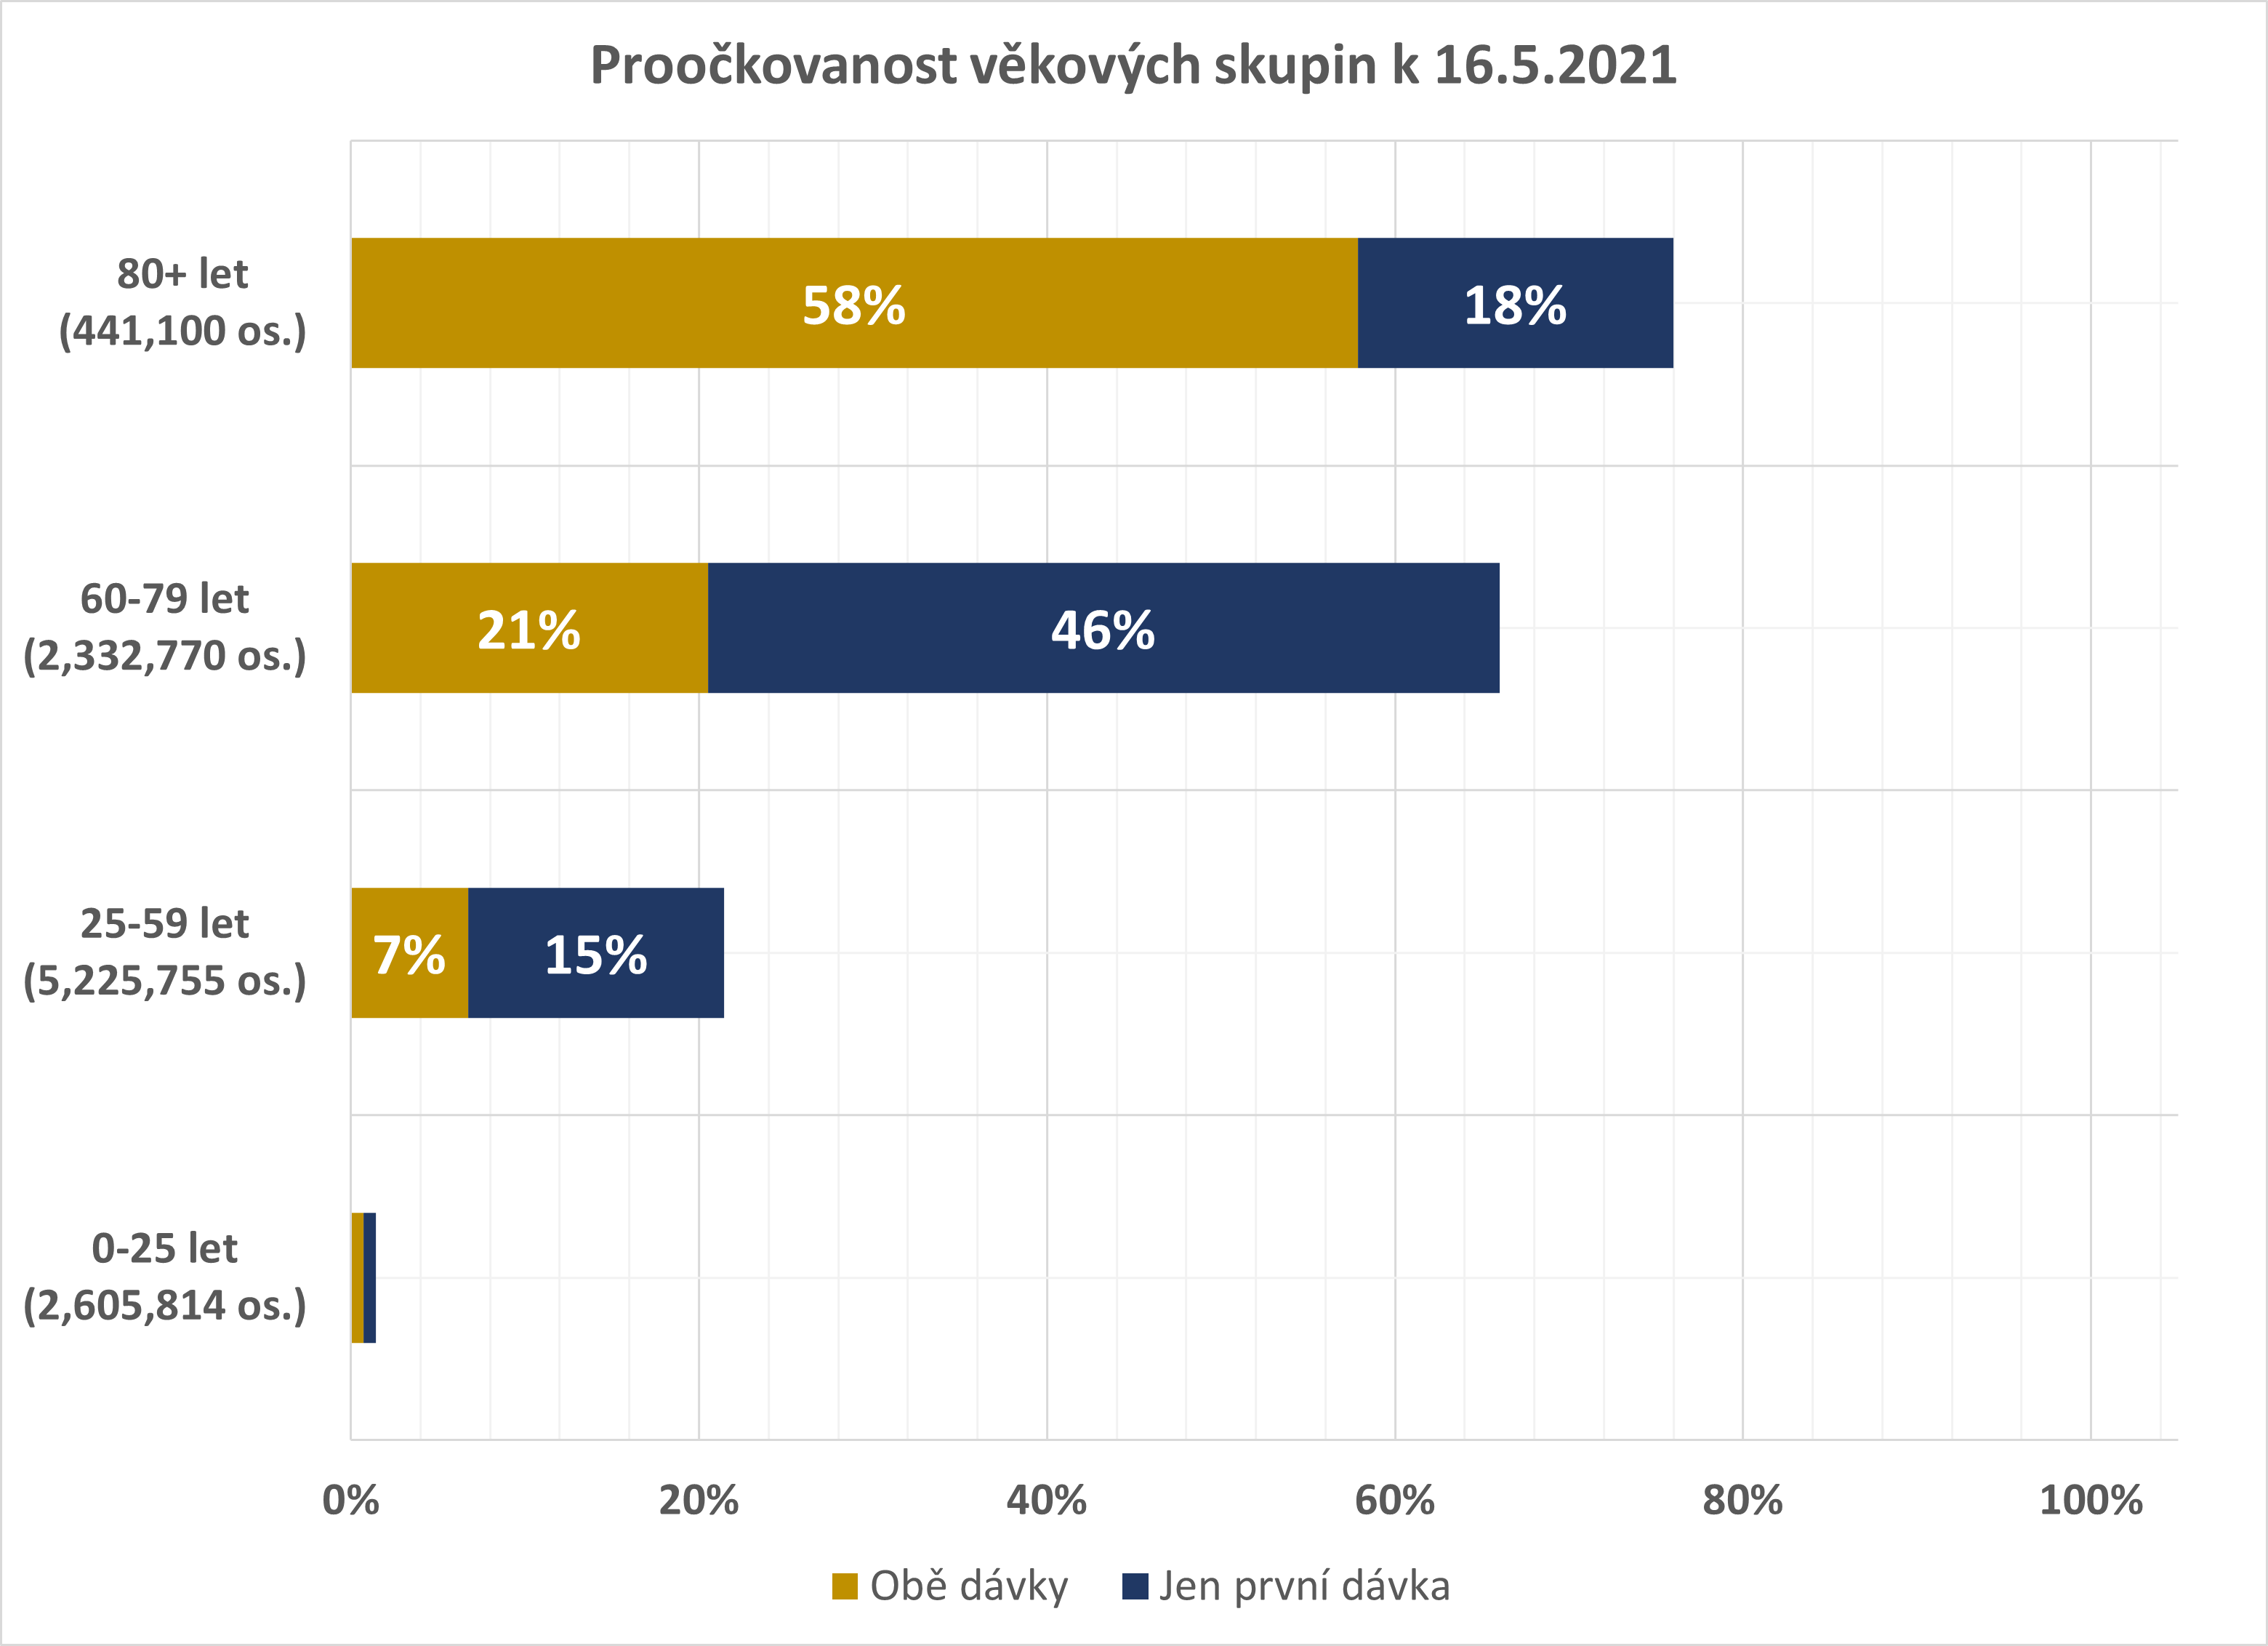
\includegraphics[height=0.3\textheight, width=\textwidth]{assets/proockovanost_veksk}
\caption{Věkové skupiny}
\label{proockovanost_vek}
\end{subfigure}



\caption{Podíly proočkovanosti věkových a prioritních skupin}
\label{proockovanost_podily}

\end{figure}



\begin{figure}
\centering

\begin{subfigure}{0.45\textwidth}
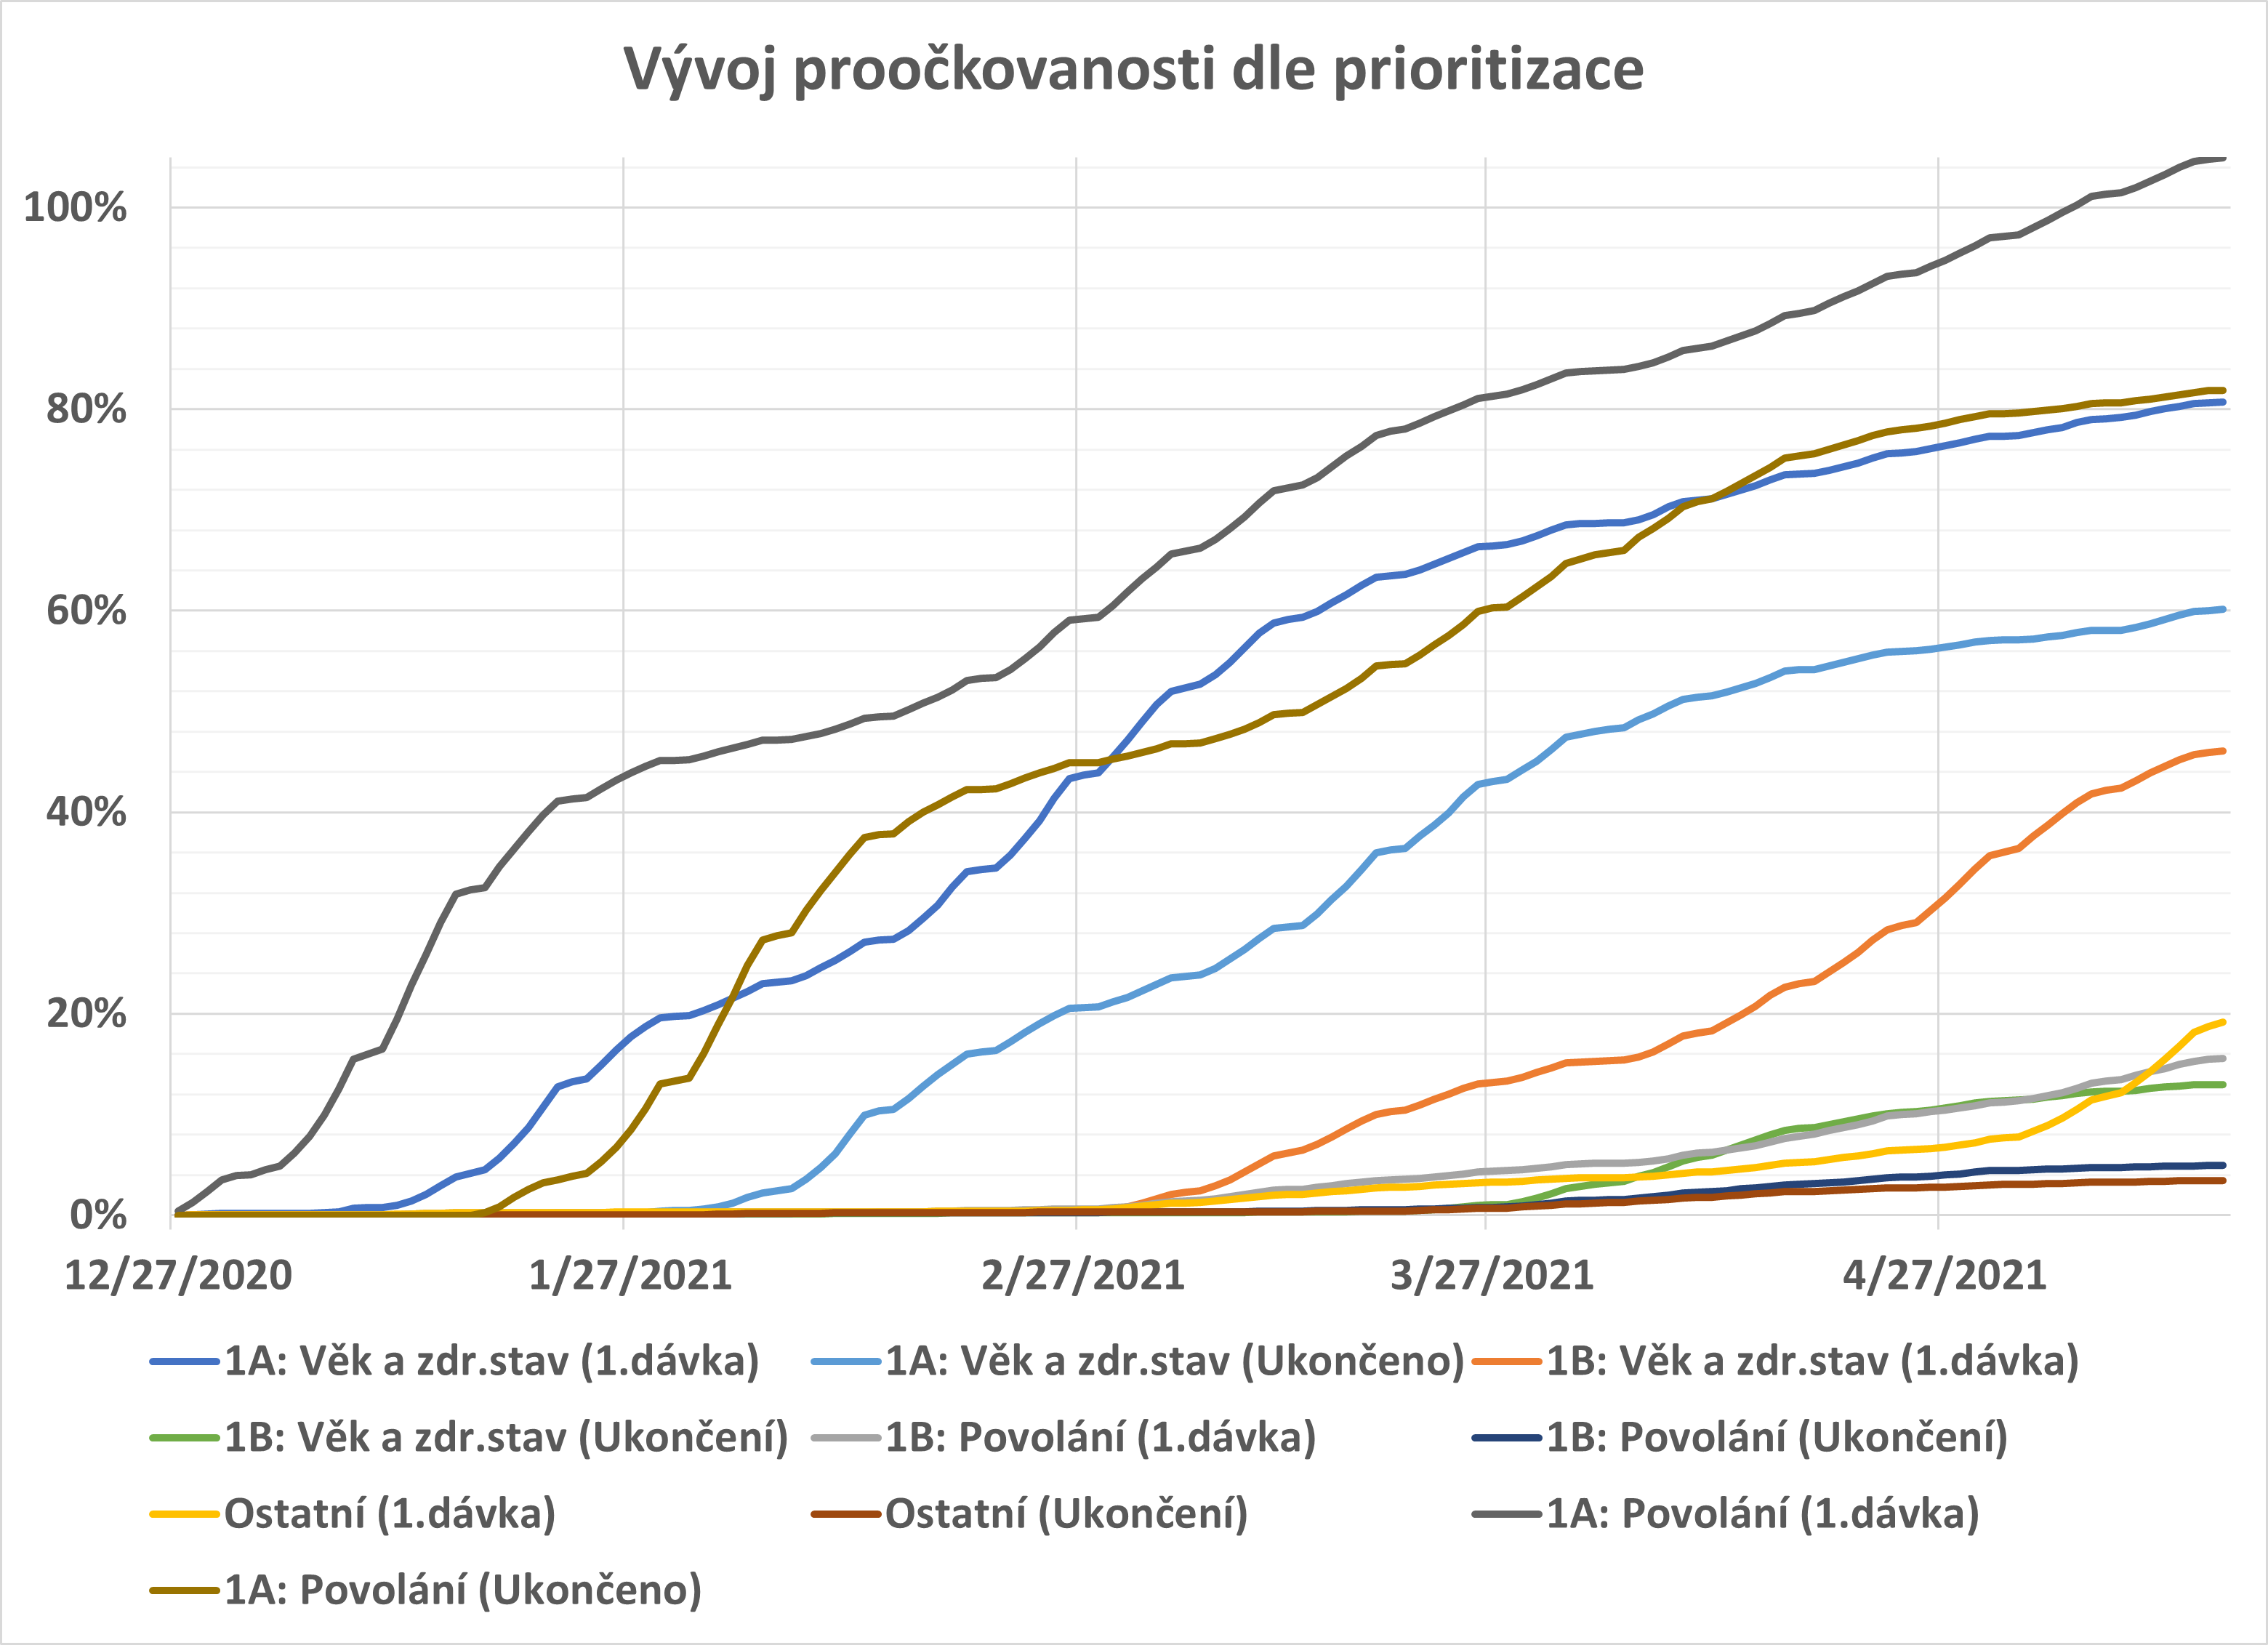
\includegraphics[width=\textwidth]{assets/gr_proockovanost}
\caption{Vývoj proočkovanosti sledovaných skupin}
\label{gr_proockovanost}
\end{subfigure}
%
\begin{subfigure}{0.45\textwidth}
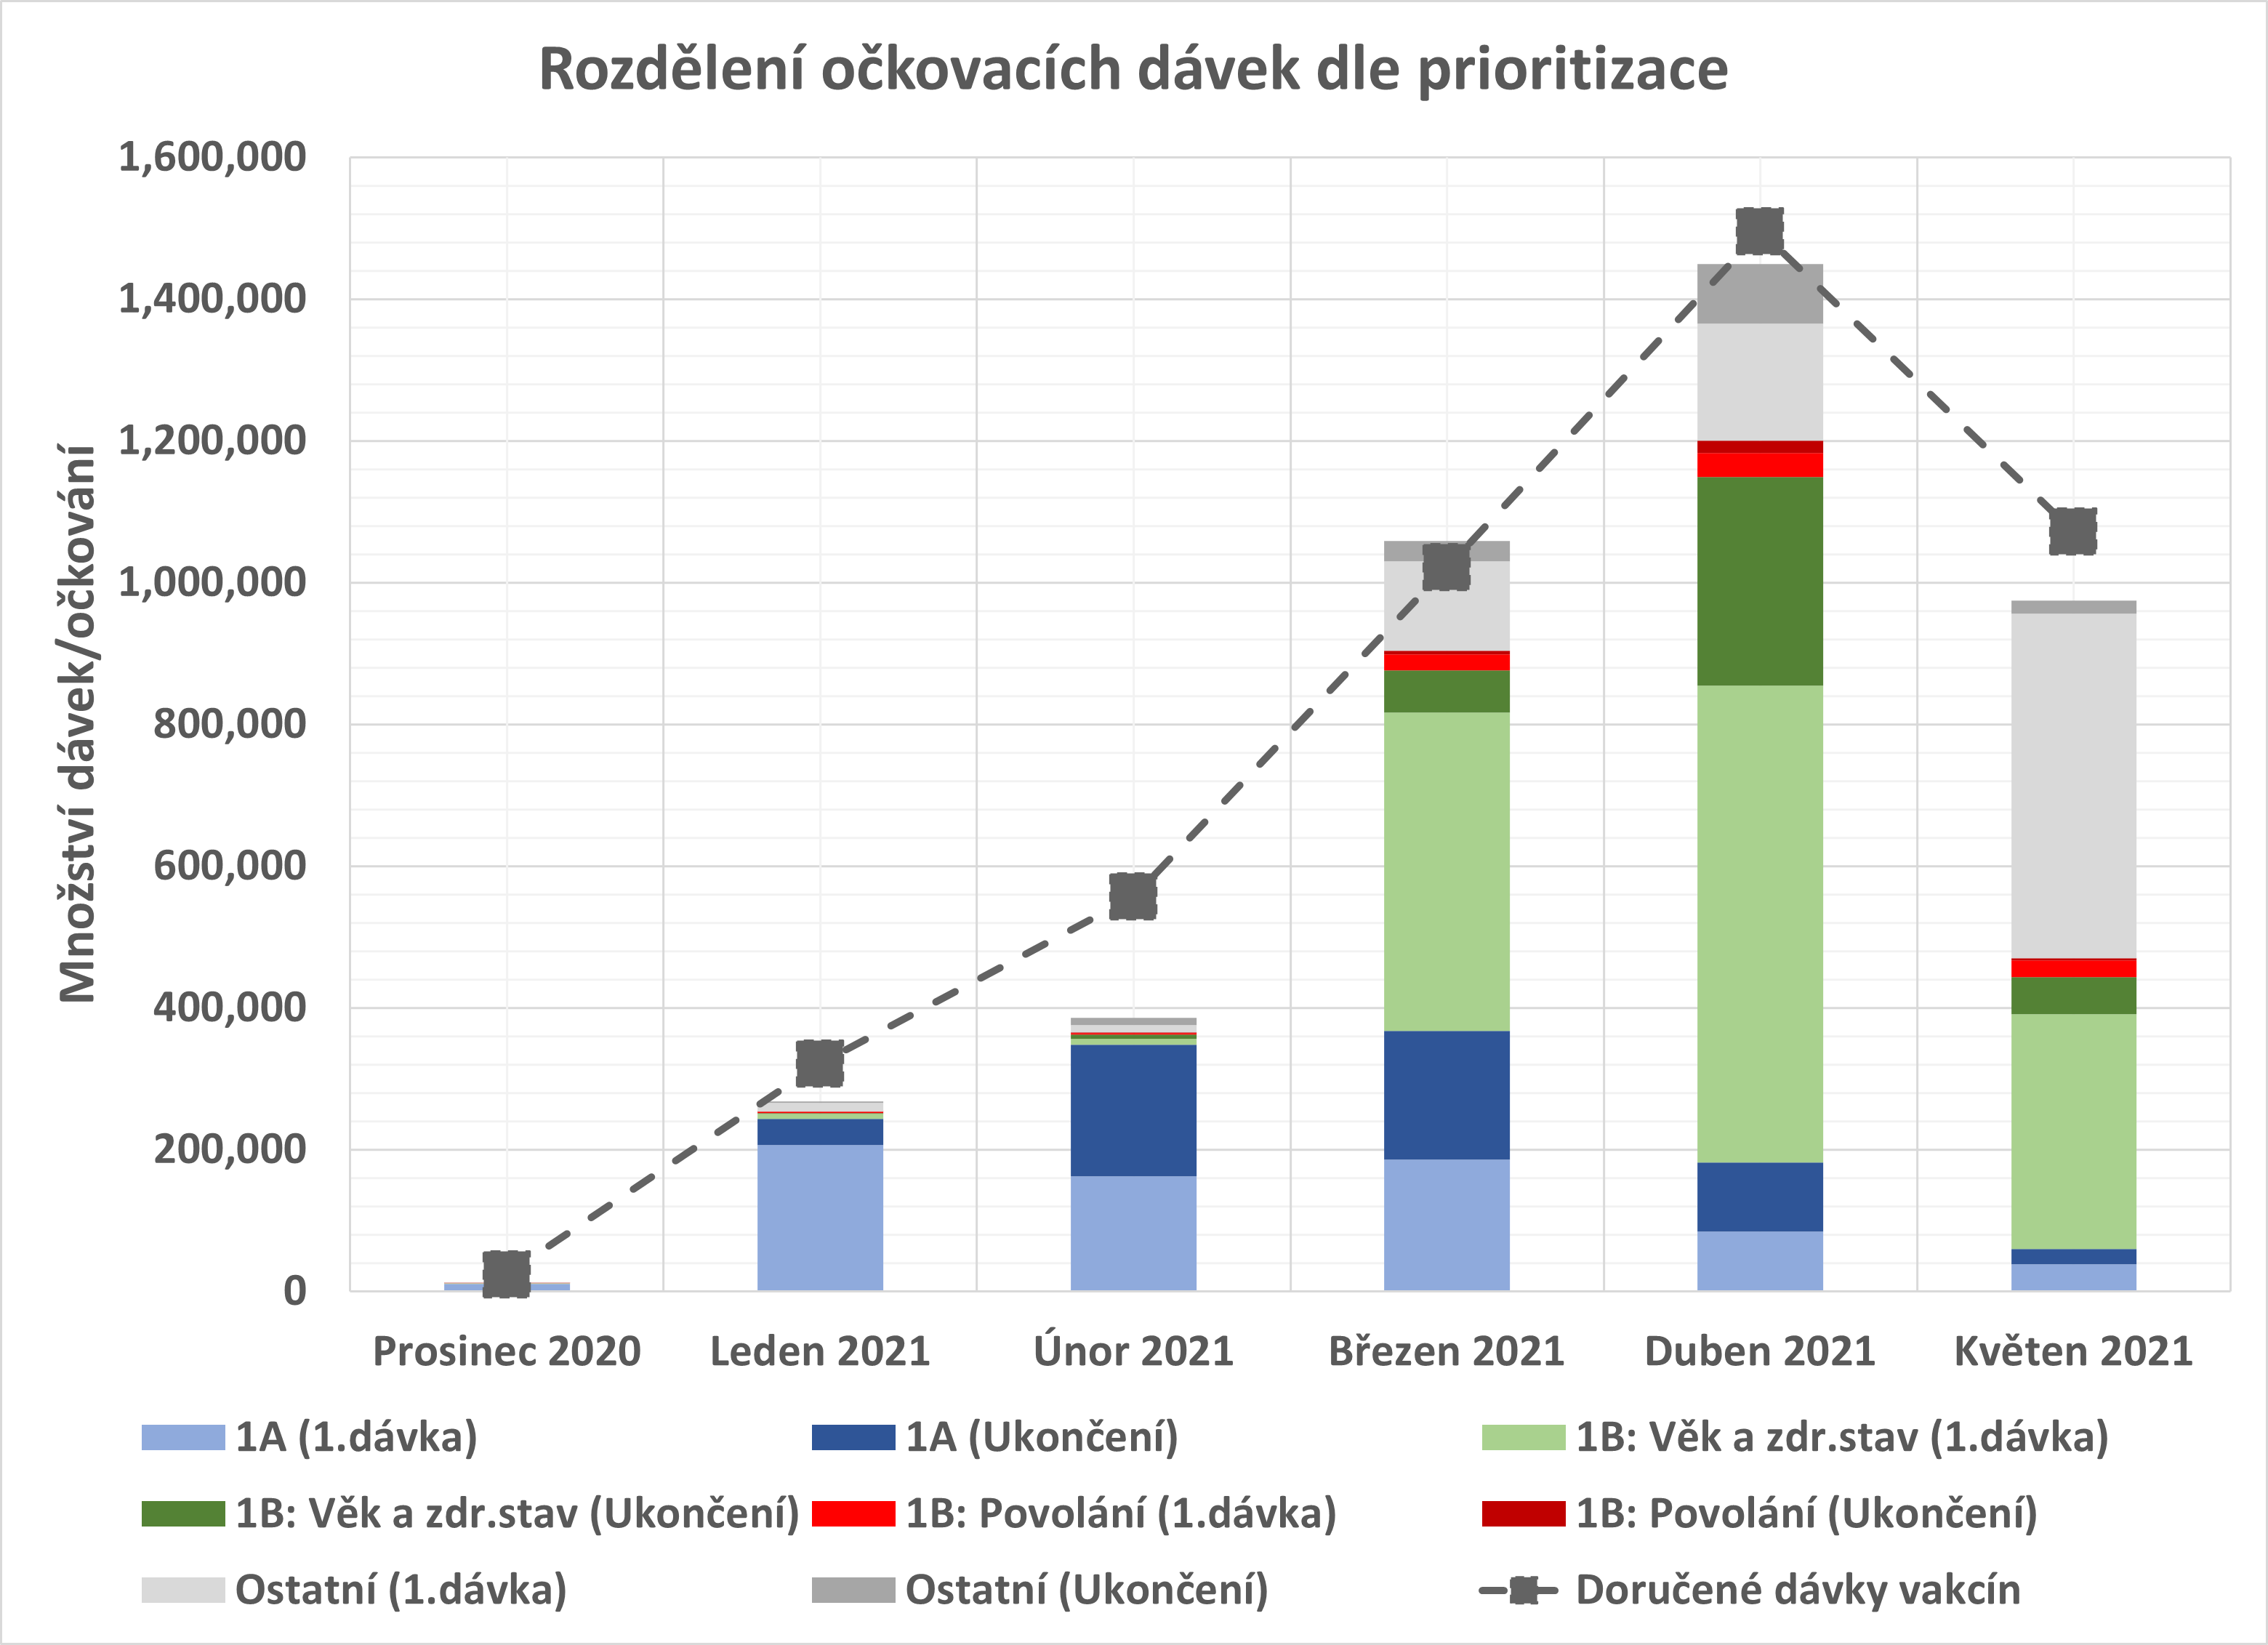
\includegraphics[width=\textwidth]{assets/gr_mesice}
\caption{Dělení dávek versus jejich celkový objem}
\label{gr_skupiny_davky}
\end{subfigure}


\begin{subfigure}{0.45\textwidth}
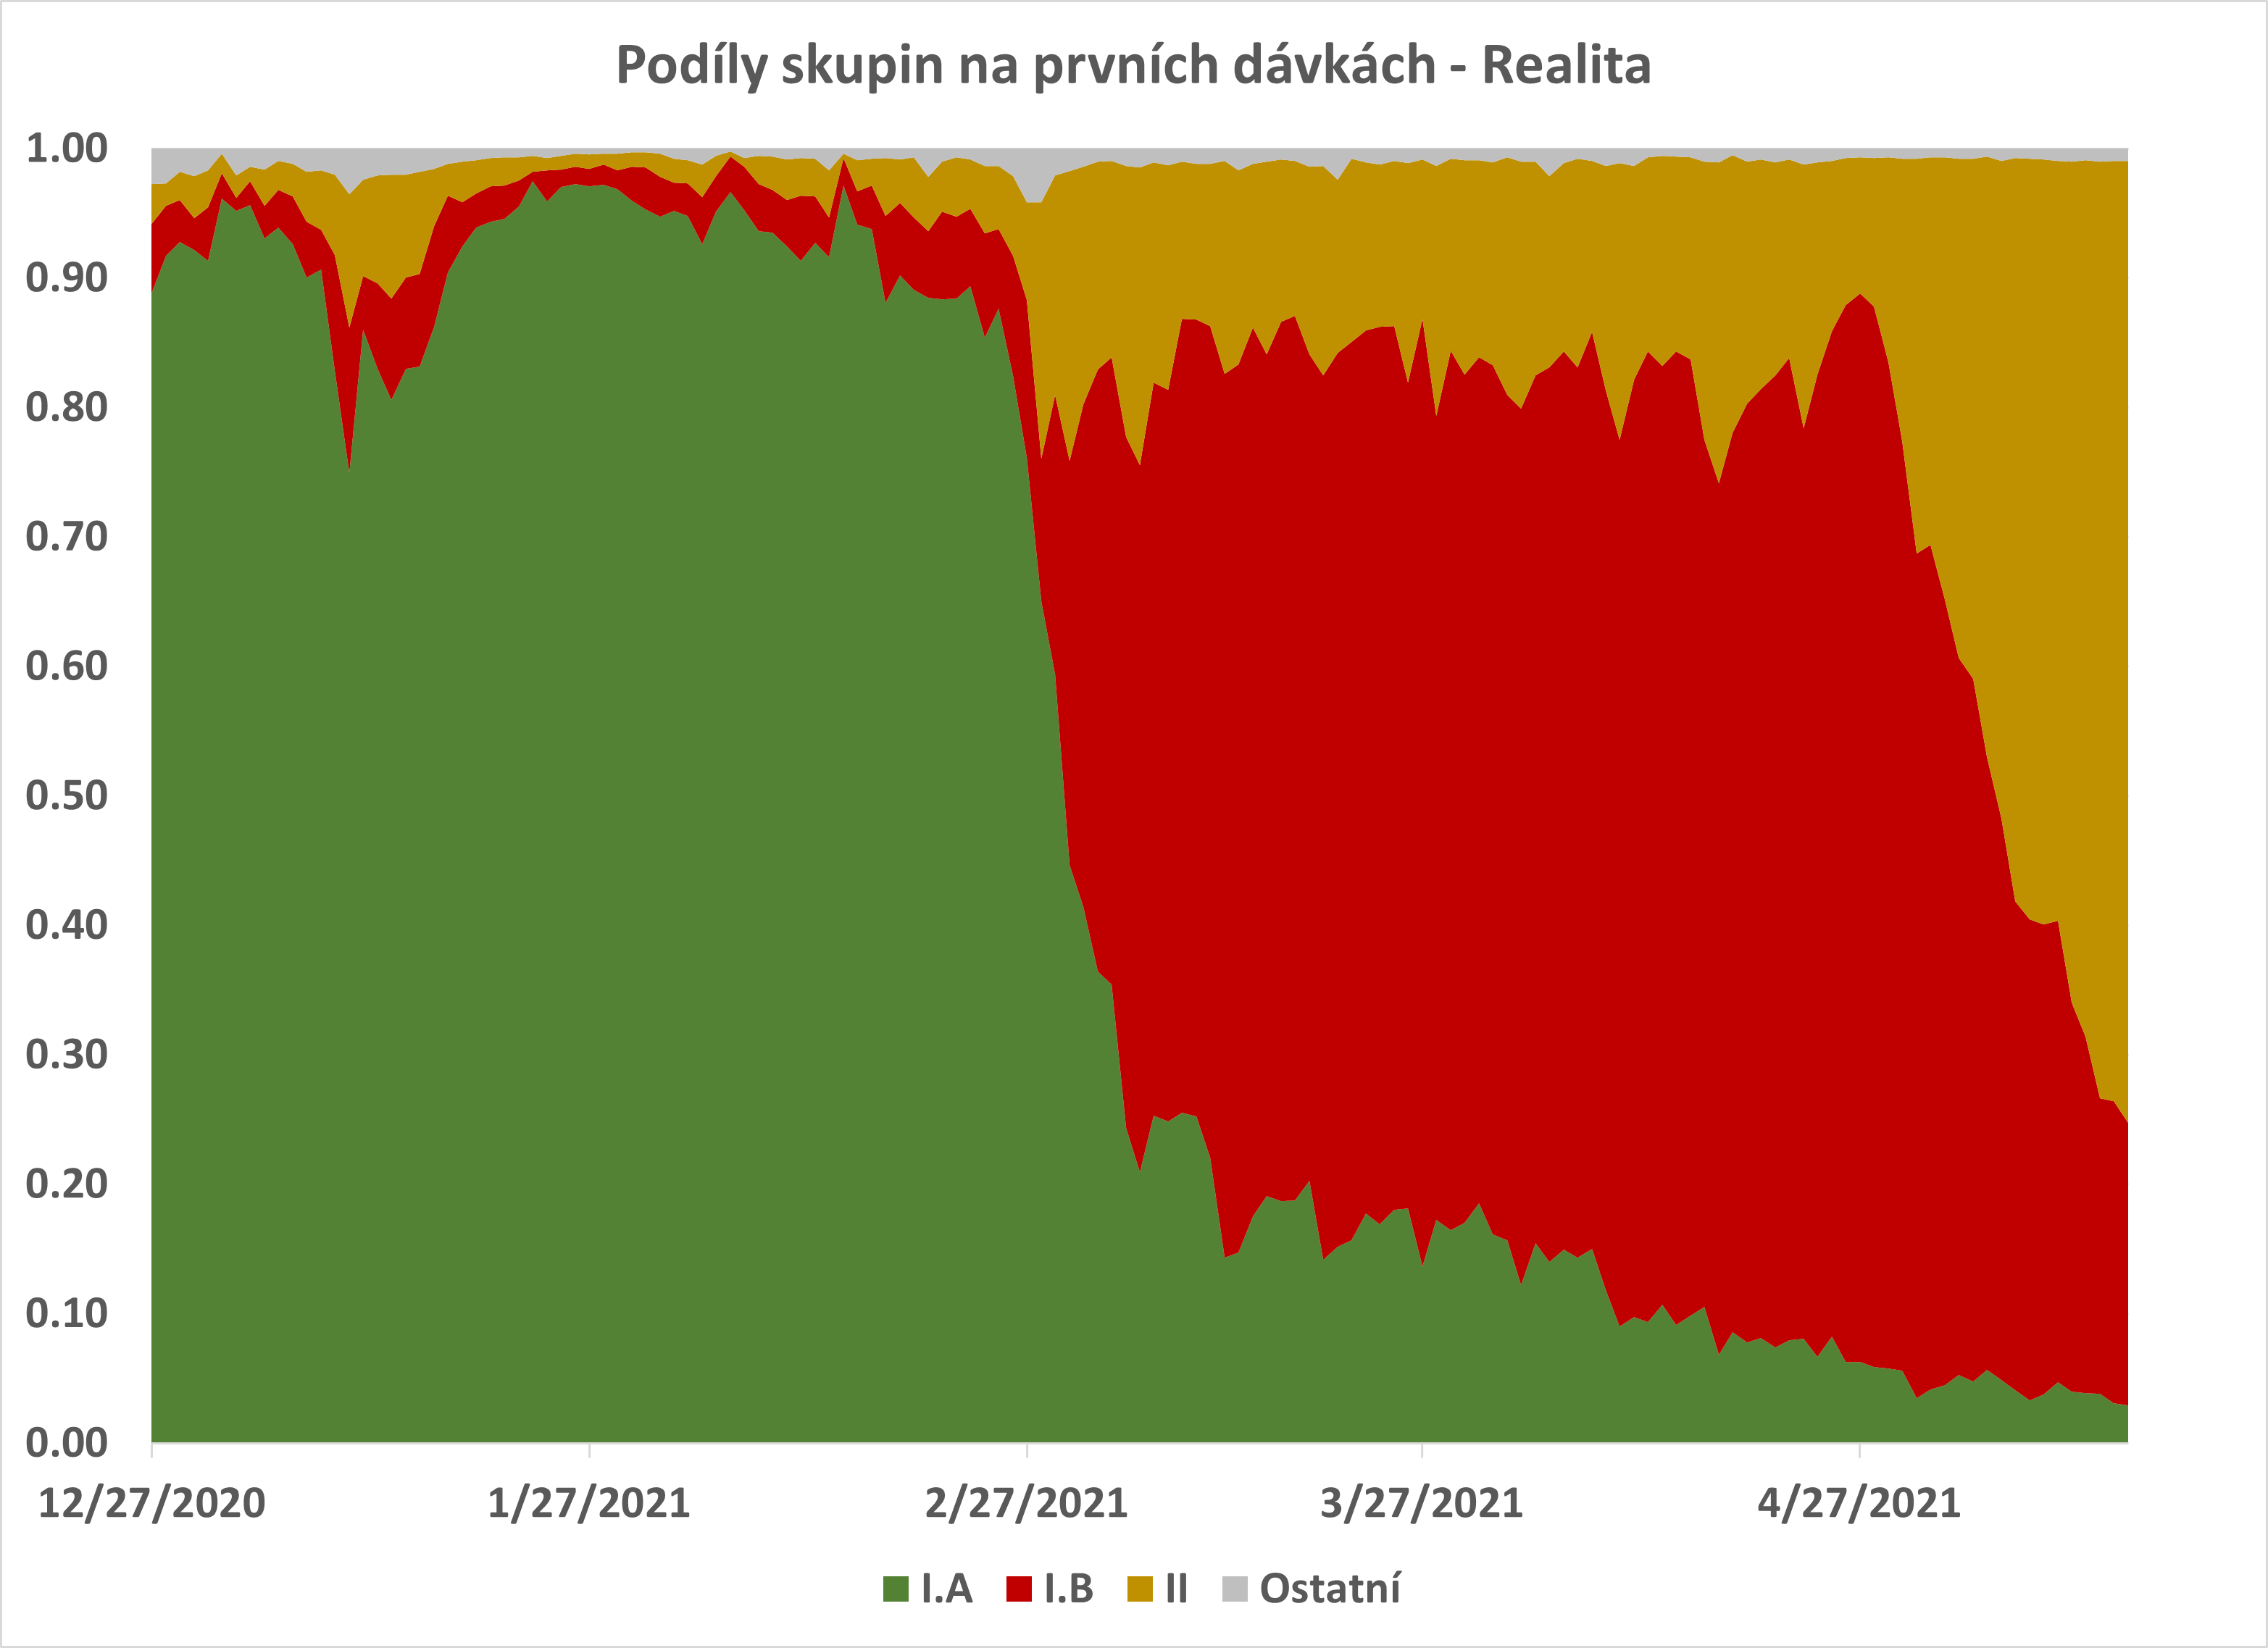
\includegraphics[width=\textwidth]{assets/theta_real}
\caption{Dělení dávek -- prioritní skupiny}
\label{gr_real_theta}
\end{subfigure}
%
\begin{subfigure}{0.45\textwidth}
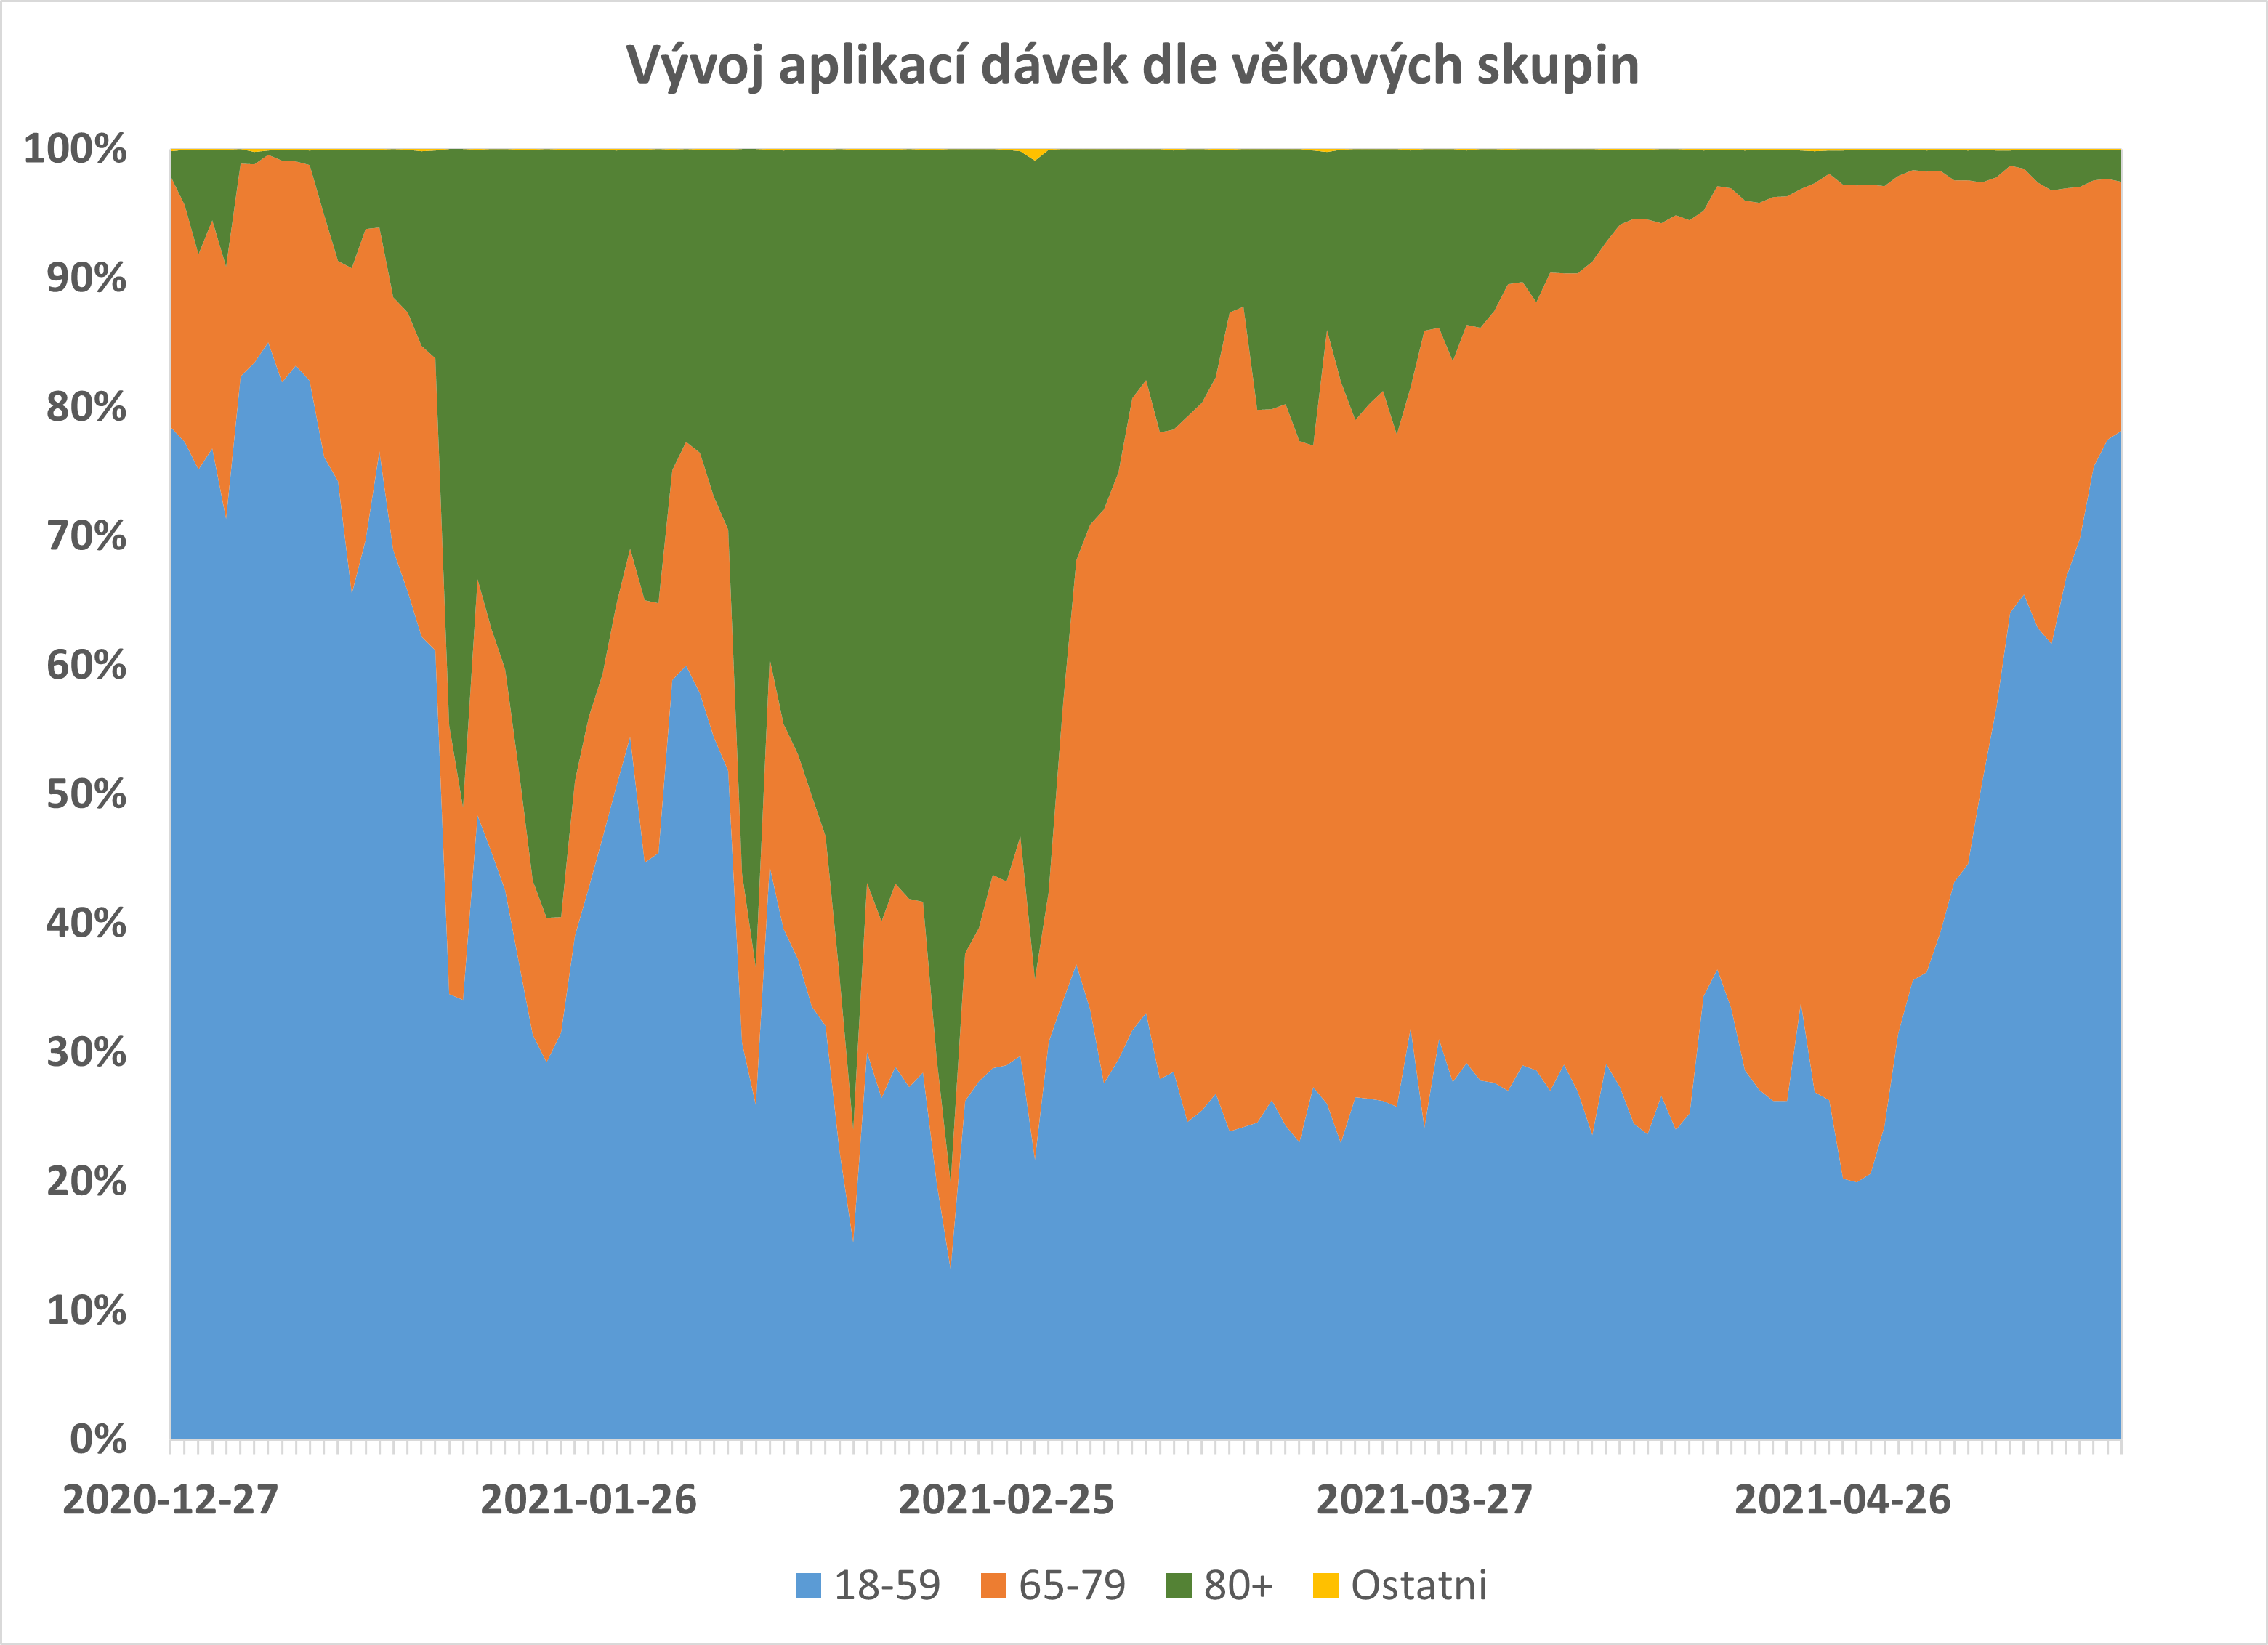
\includegraphics[width=\textwidth]{assets/chart_vek}
\caption{Dělení dávek -- věkové skupiny}
\label{gr_skupiny_davky_vek}
\end{subfigure}


\begin{subfigure}{0.45\textwidth}
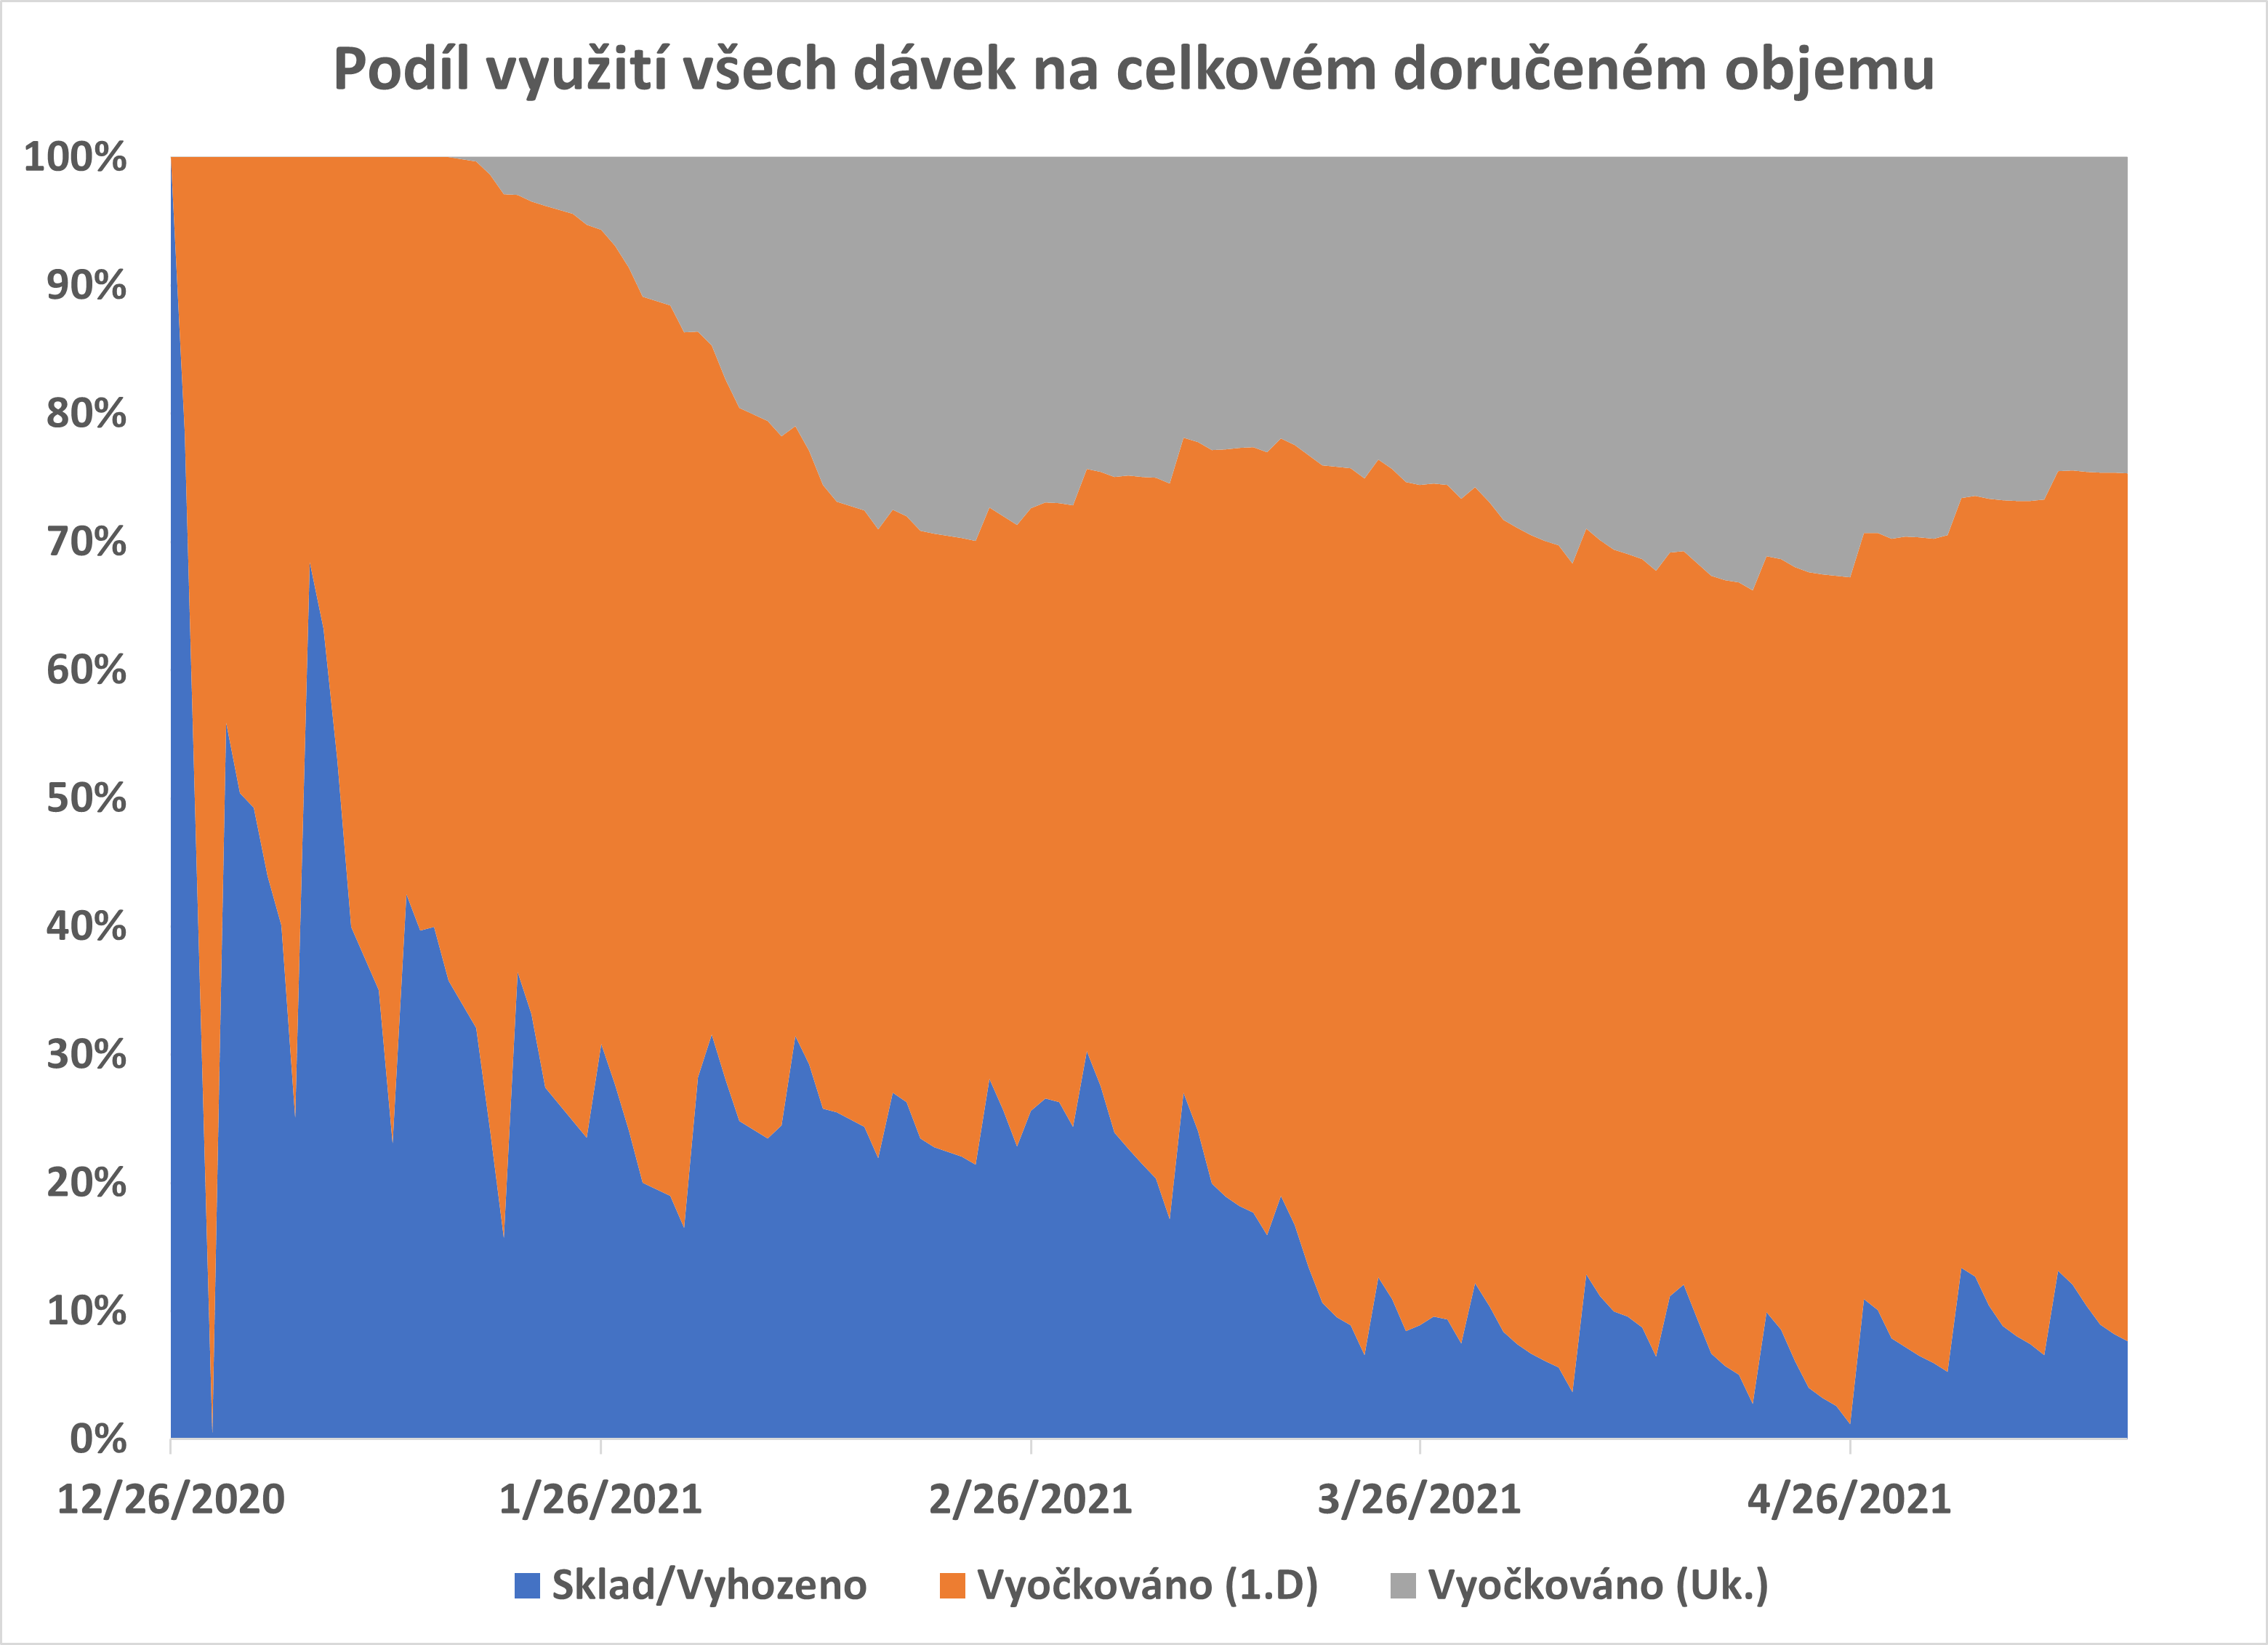
\includegraphics[width=\textwidth]{assets/gr_vyuziti}
\caption{Kumulativní vývoj skladu a způsobu využití dávek}
\label{gr_vyuziti}
\end{subfigure}
%
\begin{subfigure}{0.45\textwidth}
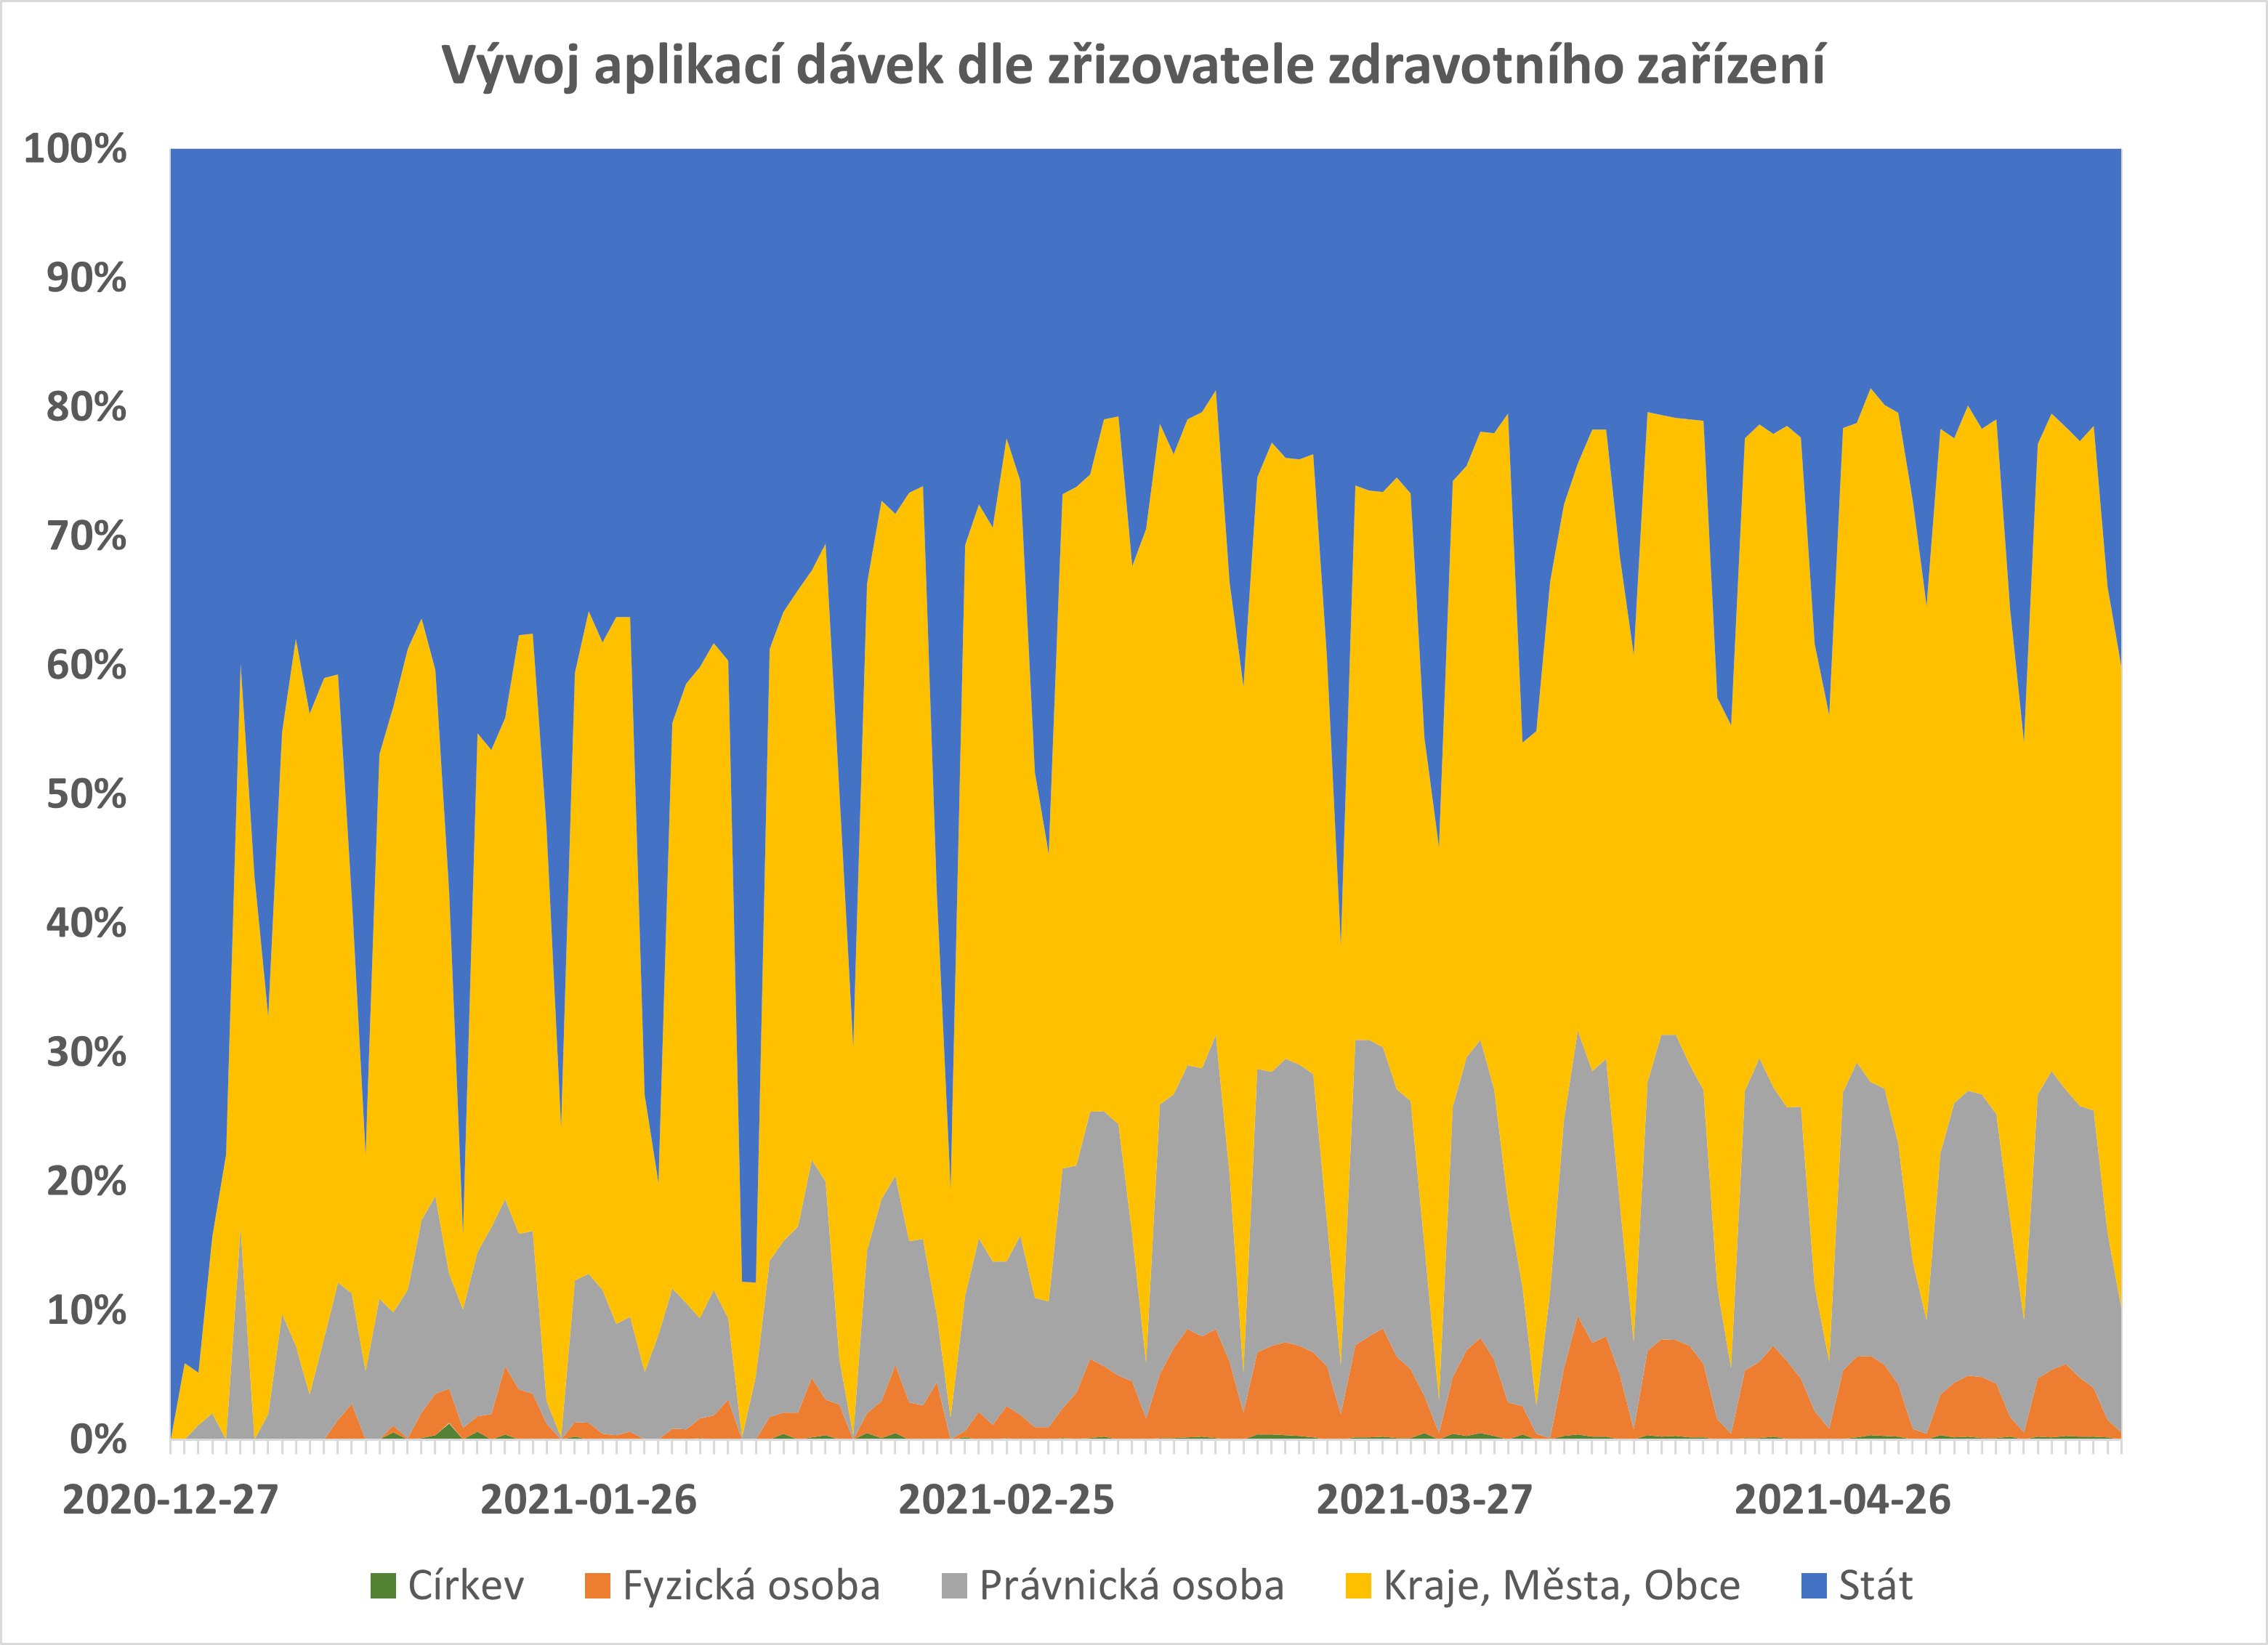
\includegraphics[width=\textwidth]{assets/chart_zrizovatele}
\caption{Podíl zřizovatelů aplikačních míst na celkovém vyočkovaném objemu}
\label{gr_vyuziti_zrizovatele}
\end{subfigure}

\caption{Reálný průběh očkování -- různé indikátory}
\label{gr_prehledy}

\end{figure}



\section*{Teoretická definice optimálního očkovacího plánu} 
\label{sec_vypocet}
%Rozdělení do prioritních skupin + rozložení vakcín v čase  + intervaly

Plánování očkování lze chápat jako optimalizační úlohu, v jejímž rámci se snažíme maximalizovat proočkovanost vybrané populace v čase. Níže popsaný postup reflektuje rozsah reálně dostupných prostředků a definuje způsob dosažení nastaveného cíle.

%Algoritmus k získání závislých proměnných $x_{t}^{1}$ (jednodávkové vakcíny aplikované v čase $t$) a $x_{t}^{2}$ (dvoudávkové vakcíny) užívá parametrů $\kappa_{t}^{1}$, $\kappa_{t}^{2}$ (denní dodávky pro jednotlivé typy vakcín), $\theta_{t}$ (kapacita očkovacích míst a $\nu$ (populace).

%Definovat si omezení (OM, dodávky, logistika)
V algoritmu pracujeme s dvoudávkovými a jednodávkovými vakcínami. Pro dvoudávkové vakcíny je definován fixní rozestup $\gamma$ mezi podáním první a druhé dávky. Pro každý z druhů vakcín dále uvažujeme kalendář dodávek -- denní přírůstky dávek jednodávkových ($\kappa_{t}^{1}$) a dvoudávkových vakcín ($\kappa_{t}^{2}$) do očkovacích míst. Dodávky $\kappa$ se přičítají do objemu vakcín dostupných ve skladech pro jednodávkové ($\alpha_{t}^{1}$), respektive dvoudávkové vakcíny ($\alpha_{t}^{2}$).\footnote{Příklad pro zjednodušení pracuje pouze s jedním druhem dvoudávkových vakcín. Jelikož se standardně nepředpokládá očkování jednoho člověka různými vakcínami, je při implementaci postupu třeba pracovat s oddělenými sklady $\alpha_{t}^{2}$ pro každý z typů dvoudávkových vakcín.} 
Samotná očkovací místa mají na úroveň jednotlivých dnů definovanou maximální kapacitu $\theta_{t}^{k}$. Součtem kapacity za všechna očkovací místa dostáváme celkovou kapacitu státu pro daný den $k=1,2 \dots K$ značenou $\theta_{t}$.
%
Velikost populace je značena $\nu$. V rámci populace lze uvažovat (v souladu se Strategií) různé prioritní skupiny $\nu_{p}$, kde $p=1,2\dots P$. Každá ze skupin $p$ má přiřazený podíl na celkovém množství rozdělovaných prvních očkování $\phi_{t}^{p}$, kde pro každé $t$ platí $\sum_{p=1}^{P}\phi_{t}^{p}=1$. 

%
Postupně pro $t=1,2 \dots T$ najdeme $x_{t}^{1},x_{t}^{2}$ (množství uskutečněných očkování pro oba typy vakcín) pomocí maximalizační úlohy

\begin{equation}
\begin{aligned}
\max_{x_{t}^{1},x_{t}^{2}}(x_{t}^{1}+x_{t}^{2})
\end{aligned}
\end{equation}

za platnosti podmínek

\begin{equation}
\begin{aligned}
x_{t}^{1}+x_{t}^{2} \leq \theta_{t}, \: \alpha_{t}^{1} \geq 0, \: \alpha_{t}^{2} \geq 0, \\
\alpha_{t+\gamma} + x_{t-\gamma}^2 \geq 0, \: \\
\sum_{\tau=1}^{t}(x_{\tau}^{1}+x_{\tau}^{2}) \leq \nu
\end{aligned}
\end{equation}

kde

\begin{equation}
\begin{aligned}
\alpha_{t}^{1}=\sum_{\tau=1}^{t}(\kappa_{\tau}^{1}-x_{\tau}^{1}) \\
\alpha_{t}^{2}=\sum_{\tau=1}^{t}(\kappa_{\tau}^{2}-x_{\tau}^{1}-x_{\tau-\gamma}^{1}) \\
\alpha_{t+\gamma}^{2}=\alpha_{t}^{2} + \sum_{\tau=t+\gamma}^{t+\gamma}(\kappa_{\tau}^{2}-x_{\tau-\gamma})
\end{aligned}
\end{equation}





%\subsection*{Identifikace optima}
%Pro každý den následně počítáme maximální počet vyočkovatelných dávek $\beta$. To se děje samostatně pro jednodávkové ($\beta{t}^{1}$) a dvoudávkové vakcíny ($\beta{t}^{2}$). Maximální počet vyočkovatelných jednodávkových vakcín je dán pouze jejich aktuálním počtem v rámci skladu $\alpha_{t}^{1}$. 
%%
%Dvoudávkové vakcíny jsou komplikovanější -- při hledání maximálního počtu je u nich totiž třeba zohlednit i \emph{rezervace} druhé dávky pro konkrétní dny ($\omega_{t}$), se kterými se počítá po uplynutí nastaveného intervalu mezi dávkami. Zásob pro druhé dávky navíc musí být v momentě, kdy jsou zapotřebí, dostatek i v případě, že by byl objem dodávek v čase klesající.
%Možný počet pro dvoudávkové vakcíny získáváme s využitím přístupu mezičasové volby\footnote{Mezičasová volba je koncept užívaný v ekonomii pro posuzování způsobu, jakým se spotřebitelé rozhodnou o konzumaci svého jmění v různých obdobích života, například za aktivního života a v důchodu. V tomto konkrétním případě se snažíme dosáhnout stejné spotřeby vakcín v rámci dvou časových úseků (dát každému pacientovi jednu vakcínu nyní a jednu po uplynutí časového intervalu).}, v jehož rámci dochází k porovnání stavu skladu \emph{dnes} se stavem \emph{po uplynutí intervalu}
%%
%Pro posouzení stavu dnes a v budoucnu jsou vypočteny pomocné indikátory $\alpha^{*}$ a $\alpha^{'}$.
%  \begin{equation*}\label{eq:alpha1}
%  \begin{aligned}
%\alpha^{*} = \sum_{t}^{t+\gamma}\alpha_{t}-\omega_{t} \\
%\alpha^{'} = min_{t}^{t+\gamma}\left | \alpha_{t} - \omega_{t} \right |
% \end{aligned}
%\end{equation*}
%%
%Maximální vyočkovatelné denní množství prvních dávek dvoudávkových vakcín je zapsáno do proměnné $\beta_{t}^{2*}$. Pokud jsou si obě hodnoty rovny či je dnešní stav nižší než stav budoucí, plánovač může vyočkovat všechny aktuálně dostupné zásoby. Pokud je dávek dnes více než v budoucnu, je v optimu vyočkována polovina celkového počtu (dnes + v budoucnu), zatímco druhá polovina zůstává pro očkování po uplynutí intervalu. Formálně popsáno:
%%
%\[
%    \beta_{t}^{2*}= 
%\begin{cases}
%    \frac{\alpha^{*}+\alpha_{t}}{2},& \text{pokud } \alpha_{t}>\alpha^{*}\\
%    \alpha_{t},& \text{jinak}
%\end{cases}
%\]
%%
%V dalším kroku do úvahy vstupuje omezení dané celkovou kapacitou očkovacích míst $\theta_{t}$. Nalezením minima mezi ním a optimálním počtem všech (dvoudávkových i jednodávkových) vakcín získáváme počet očkování, jež lze v daný den reálně uskutečnit.
%Tento počet je následně rozdělen mezi všechny tři režimy očkování. Nejvyšší priorita je dána druhým očkováním (pro dodržení předepsaného intervalu), druhá v pořadí jsou očkování jednodávkovými vakcínami (jejichž použití vede k dřívějšímu ukončení očkování, než pokud očkovaný musí čekat na druhou dávku) a zbylá kapacita je využita k prvnímu očkování dvoudávkovými vakcínami.
%%
%Způsob výpočtu množství ve výsledku aplikovaných vakcín je uveden níže. Krom již zmiňovaných omezení do výpočtu dále vstupuje zbylá potřeba prvních dávek v daný čas $\nu_{t}$.
%%
%\begin{equation*}\label{eq:beta}
%\begin{aligned}
%\omega_{t}=min(\theta_{t},\omega_{t}^{*})\\
%\beta_{t}^{1}=max(\nu_{t},min(\theta_{t}-\omega_{t}),0) \\
%\beta_{t}^{2}=max(\nu_{t},min(\beta_{t}^{2*},[\theta_{t}-\beta_{t}^{1}-\omega_{t}]),\alpha^{'},0)
%\end{aligned}
%\end{equation*}
%%
%Výsledný denní počet dávek k vyočkování je tedy roven $\beta_{t}=\omega_{t}+\beta_{t}^{1}+\beta_{t}^{2}$. 
%

%\subsection*{Dělení dávek do prioritních skupin}
%Dostupné dávky je dále třeba rozdělit mezi cílové příjemce -- osoby v rámci prioritních skupin. Druhé dávky dvoudávkových vakcín $\omega_{t}$ jsou přiděleny dle stejného klíče, jako byly před stanoveným intervalem $\gamma$ děleny první dávky ($\beta_{t-\gamma}^{2}$). První dávky dvoudávkových vakcín $\beta_{t}^{2}$ a jednodávkové vakcíny $\beta_{t}^{1}$ jsou celočíselně rozdělovány do $1,2,...P$ prioritních skupin $p$, a to tak, že je pro každou skupinu stanoven podíl na celku $\phi_{t}^{p}$, kde platí $\sum_{p=1}^{P}\phi=1$. V případě, že je některá ze skupin v daném časovém momentě již doočkovaná či skupina už jen čeká na uplynutí intervalu pro druhé očkování ($\nu{t}^{p}=0$), je podíl ostatních skupin v daný den nanormován do 1.
%
%Po nalezení množství uskutečnitelných očkování probíhá rozdělení vakcín mezi jednotlivé prioritní skupiny. Každé ze skupin je přidělen podíl na celkovém úhrnu vakcín, který je po doočkování skupiny (či v momentě, kdy skupina už jen čeká na uplynutí intervalu pro druhé očkování) anulován a poměr ostatních skupin znovu nanormován na 100 \%. 
%Současně s naplánováním očkování dvoudávkovými vakcínami je zapsána hodnota $\omega_{t+\gamma}$ spolu s příslušnými podíly $\phi*_{t+\gamma}^{p}$, s jejichž pomocí se zajišťuje uchování potřebného počtu vakcín pro vyočkování druhých dávek, respektive jejich rozdělení na ně čekajícím příjemcům.% ze skladu $\alpha_{t+\gamma}^{2}$ pro den po uplynutí nastaveného intervalu mezi dávkami odečteno množství vakcín, které bude v daný den potřeba k vyočkování ve formě druhých dávek.

%\subsection*{Aplikabilita přístupu}
 %Pokud mají očkovací místa výkyvy kapacity na základě dnů v týdnu (typicky omezený provoz o víkendu), hodí se dále pracovat s intervaly mezi dávkami v celých týdnech. Tím se zamezí tomu, aby byly například na neděli naplánovány vakcinace pro očkování neúměrného počtu lidí. 

Dále také platí $x_{\tau}=0$ pro $\tau<1$.
Celý algoritmus je tedy velice jedoduchou úlohou lineárního programování, kterou je schopen řešit například Microsoft Excel\footnote{Celý přístup byl skupinou autorů již dříve právě za účelem jeho reálného užití v plánování popsán a do MS Excel implementován \cite{calc_blog}.}. Algoritmus lze při korektním zadání vstupních dat užívat pro plánování na libovolné úrovni: státu, kraje či jednotlivého očkovacího místa. 



%
%Představený algoritmus by při nekonečné kapacitě očkovacích míst a dostatku dávek už na začátku operace vedl k očkování celého státu ve dvou dnech, kdy v prvním by byly vyočkovány všechny jednodávkové vakcíny a polovina dvoudávkových vakcín. Po uplynutí intervalu by byla vyočkována druhá polovina dvoudávkových vakcín.

\section*{Srovnání reálného a teoretického přístupu}
%Porovnání optimálního scénáře s realitou + distribuce vakcín
%Tato sekce projde grandma testem
%Co nejméně věcí, jen ty podstatné. Grafy, tabulky
%Identifikace frikcí mezi potenciálně optimálním nastavením a realitou

%Blízkost reality k teoretickému optimu je dána nejen omezeními reálného světa (nedosažitelností nekonečných skladovacích a aplikačních kapacit stejně jako nekonečného množství očkovacích dávek), ale i politickými a administrativními rozhodnutími v některých otázkách. Zmíněná rozhodnutí mohou do plánování vstupovat jako parametry ovlivňující účinnost celé operace či jednotlivé v ní sledované veličiny.
%
V rámci této sekce jsou na reálných datech o průběhu očkování odhadovány klíčové parametry, tedy stavy skladu $\alpha$, prioritizační podíly $\phi^{p}$ a zejména optimální objemy očkování $x_{t}^{2*}$. Identifikované hodnoty jsou dále dány do kontrastu s optimem dle teoretické definice představené v sekci \ref{sec_vypocet}. 
Cílem porovnání je identifikovat blízkost teoretického optima a reálného průběhu kampaně v České republice.




\paragraph{Metoda porovnání: }\label{sec:comparison}V porovnání jsou uvažovány dva scénáře (\emph{MOD1, MOD2}), které  jsou generovány mechanismem dle definice v předchozí sekci. Oba scénáře pokrývají pouze historii, tedy dobu mezi 26. 12. 2020 (zapsání prvních očkovacích dávek do systému) a 16. 5. 2021 (ohraničení dat pro analýzu).
Veškerá využitá data pocházejí z otevřených zdrojů poskytovaných Ministerstvem zdravotnictví ČR \cite{mzcr_data}, ve kterých nicméně nejsou obsaženy informace o maximální možné kapacitě očkování v daný den. 



%První scénář, \emph{Realita} vznikl kalibrací výpočtu dat o vykázaných očkováních a dodaných dávkách. 


\emph{MOD1} počítá se třemi kapacitami (všední den, sobota, neděle). Kapacity v modelu nikdy zpětně neklesají, tzn. denní kapacita je určena jako maximum kapacity z %modelu \emph{Realita} a 
všech předcházejících vyočkovaných objemů dle empirických dat pro všední den/sobotu/neděli. \emph{MOD1} má dále napříč dny stanoveny podíly $\phi$ pro skupinu I.A na 95 \%, pro I.B na 4 \% a pro II. na 1 \%.
%
\emph{MOD2} používá stejné podíly  $\phi$ jako \emph{MOD1} a vedle toho uvažuje situaci, kdy by již od začátku očkovací kampaně byly kapacity rovny identifikovanému maximu (samostatně pro všední dny, soboty a neděle) do 16. 5. 2021. 
%
Cílové míry proočkovanosti jsou pro oba scénáře stanoveny na 95 \% pro I.A, 70 \% pro I.B a 60 \% pro II. Parametr intervalu mezi dávkami dvoudávkových vakcín $\gamma$ je nastaven na 42 dnů.


Modelové scénáře \emph{MOD1} a \emph{MOD2} jsou pro srovnání doplněny o třetí scénář, označený jako \emph{Realita.}  Ve scénáři \emph{Realita} jsou prioritizační poměry $\phi$ nastaveny dle vykázaných prvních očkování. Jak už bylo uvedeno výše, z dostupných dat nelze jasně určit maximální možnou kapacitu pro určitý den. Pro její aproximaci v kontrolním scénáři \emph{Realita} počítáme využití kapacit ze 100 \%, tedy že počet aplikovaných dávek přesně odpovídal kapacitě v daný den.
%Scénáře jsou dále srovnány s reálně dosaženými hodnotami (označení \emph{Realita}).




%\textbf{MOD2 popisuje zcela optimální (nekonečné kapacity očkovacích míst) a omezený nedostatkem kapacit}\footnote{V této variantě je kapacita odhadována z reálných dat. Předpokládá se, že celková kapacita očkovacích míst ($\theta_{t}$ dle notace v pojednání k výpočtu) pro všední den/sobotu/neděli nikdy neklesá. Její hodnota je tedy vždy udána jako maximum zaznamenané kapacity od začátku očkování do daného dne.}.
%Vlastnosti prioritních skupin, jejich poměry na rozdělovaných dávkách a cílové proočkovanosti jsou nastaveny v souladu se Strategií očkování, Metodickým pokynem a jejich reportovanými úpravami \cite{strategie_covid,ockovani_mp,mzcr_0516}. Porovnání se tedy (přinejmenším v této části stati) nezabývá nastavením prioritizace (užita je inovovaná verze prioritizačního schématu z 26. 4. 2021), ale dívá se na prioritní skupiny striktně dle původního záměru daného Strategií a Metodickým pokynem. Důraz je tedy kladen na co nejrychlejší proočkování skupin ohrožených těžkým průběhem nemoci, respektive úmrtím. 
%


\paragraph{Shrnutí výsledků porovnání:} Na grafech přiložených k článku jsou ukázány výsledny srovnání obou scénářů a empirických dat. Horní dva grafy sledují problematiku využití dostupných dávek. Graf \ref{gr_mod_vyockovanost} zobrazuje procentuální vyprázdněnost skladu. Graf \ref{gr_models_delta} celkové množství vyočkovaných dávek v modelech \emph{MOD1} a \emph{MOD2} v porovnání s reálnými daty.
%
Spodní dva grafy jsou zaměřeny na prioritizaci.
Graf \ref{gr_mod_prvni_davka} zobrazuje vývoj proočkovanosti nejkritičtější skupiny I.A. Na grafu  \ref{gr_mod2_theta} je pak vidět vývoj rozdělení prvních dávek do tří prioritních skupin v rámci \emph{MOD2}.
%Na grafu 


\begin{figure}
\centering


\begin{subfigure}{0.45\textwidth}
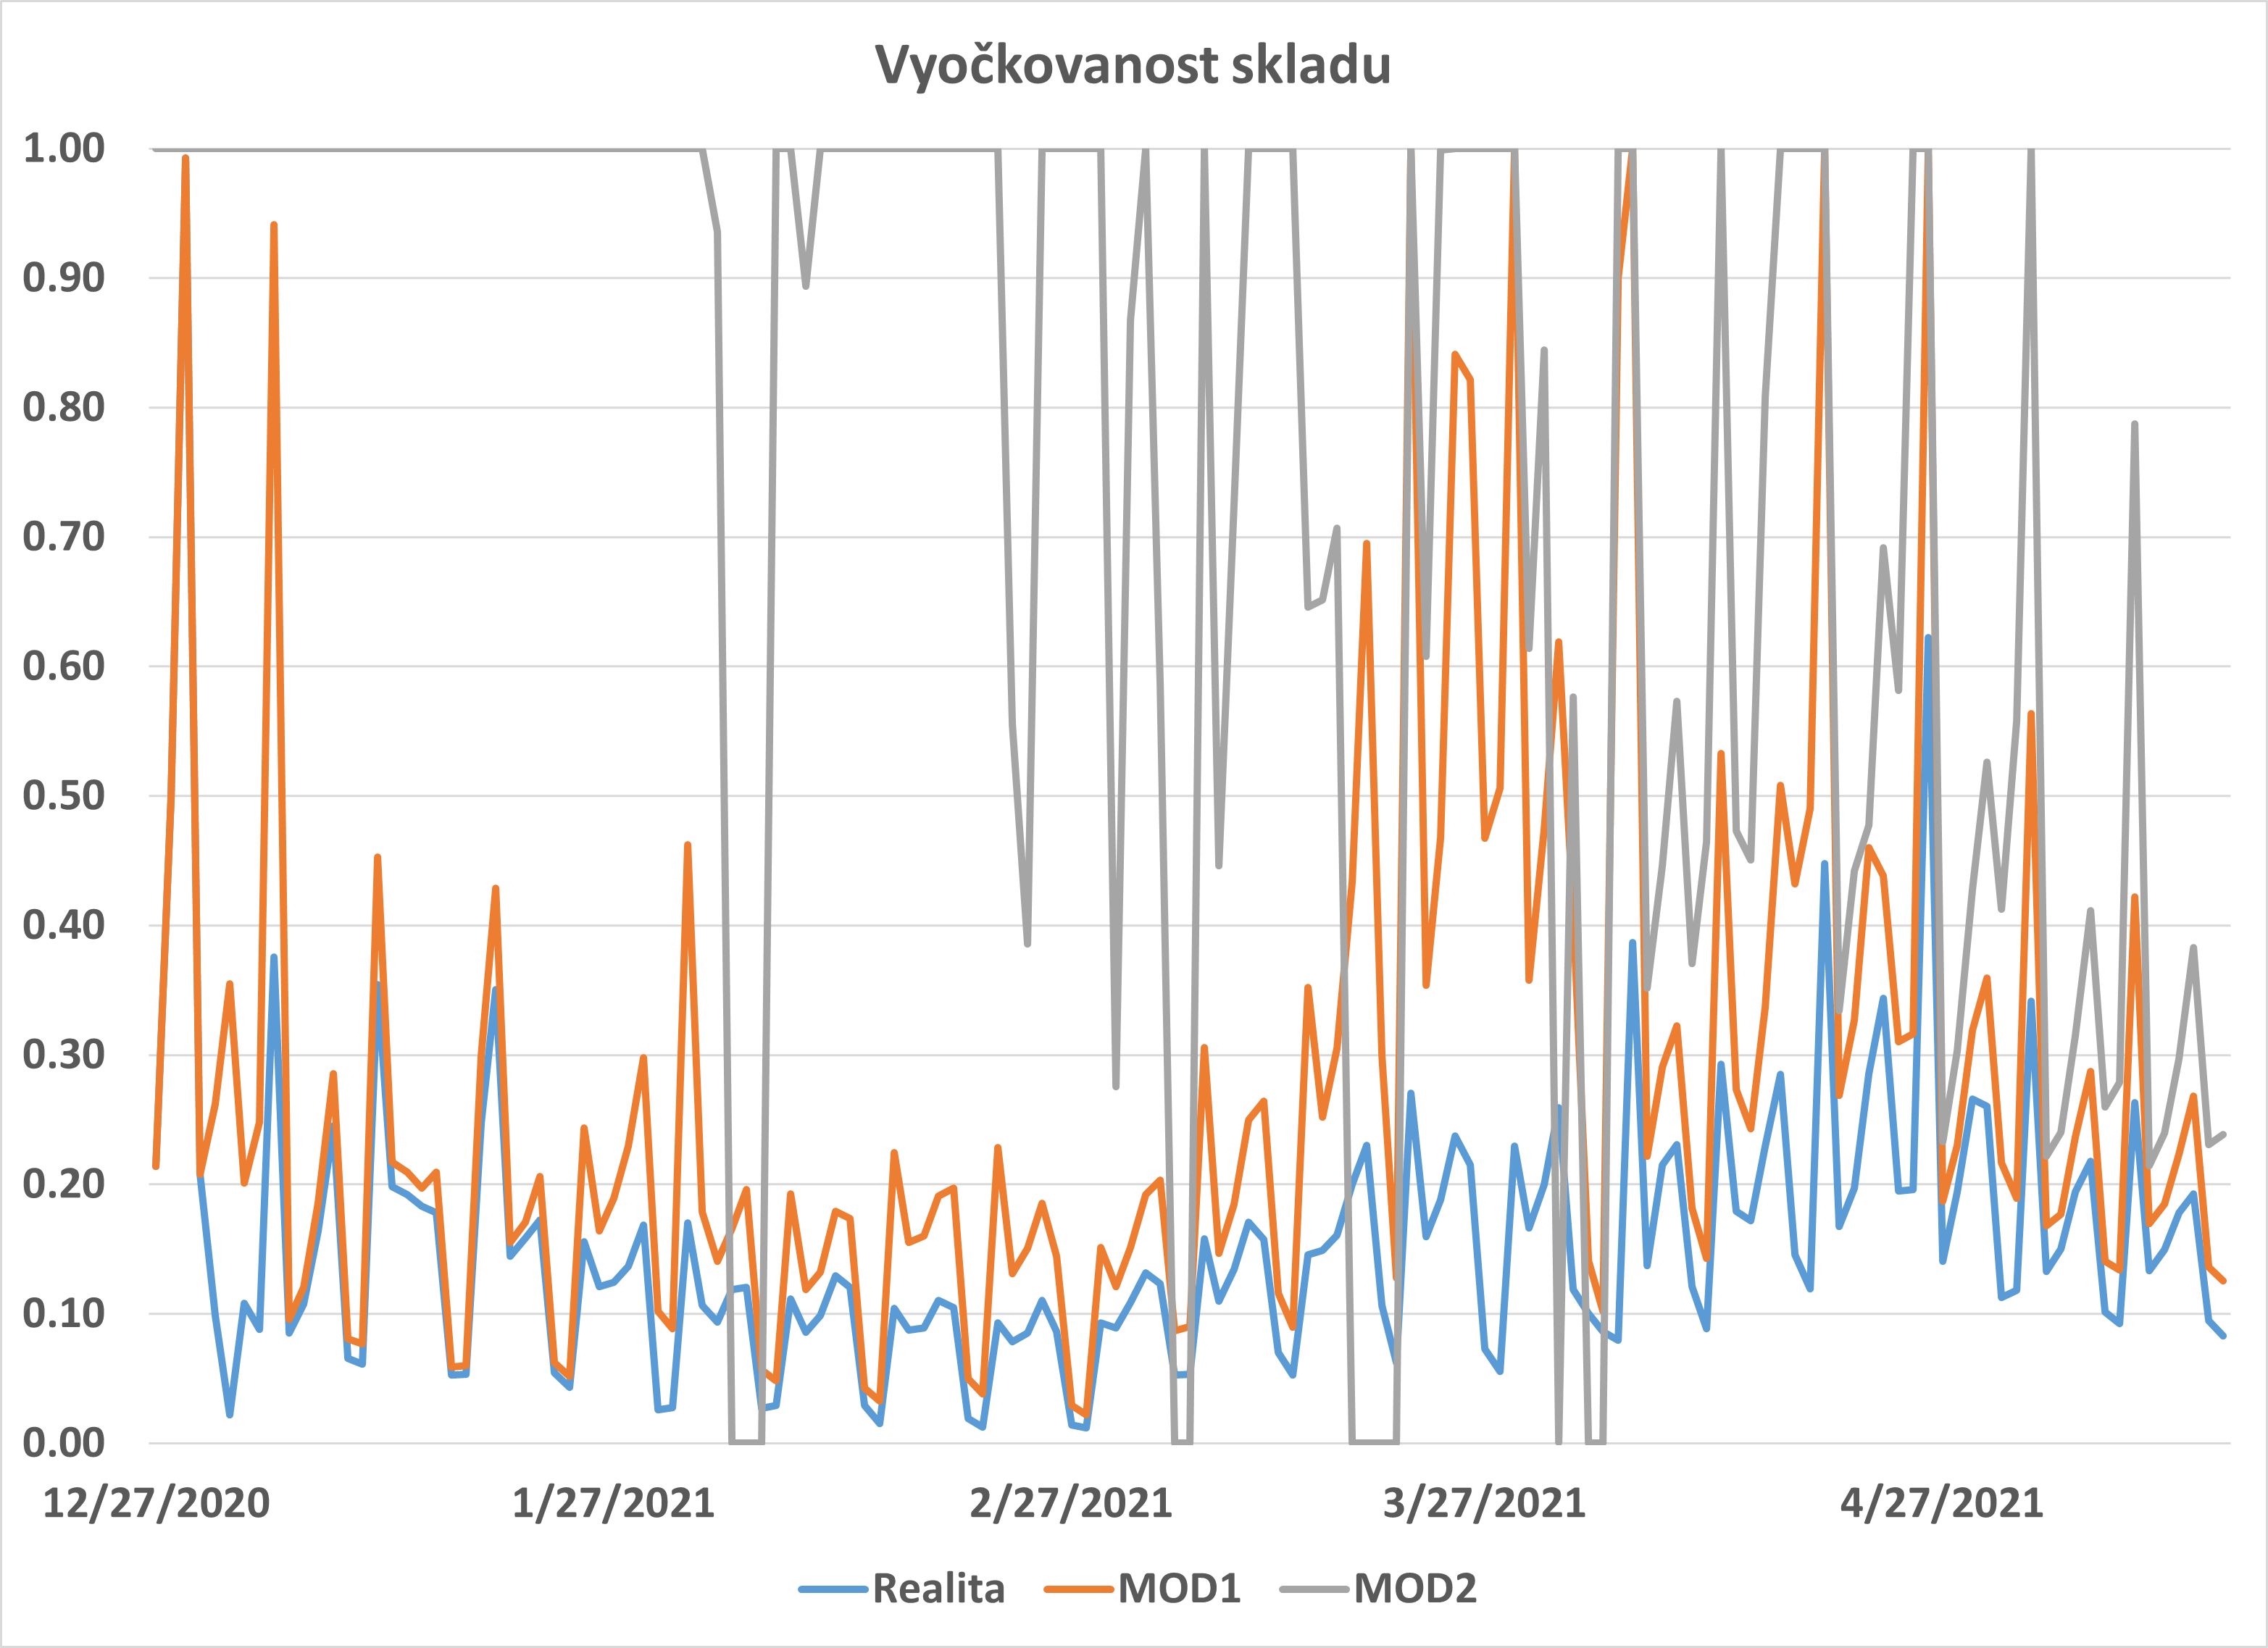
\includegraphics[width=\textwidth]{assets/sklad_vyockovanost}
\caption{Stav vyprázdněnosti skladu}
\label{gr_mod_vyockovanost}
\end{subfigure}
%
\begin{subfigure}{0.45\textwidth}
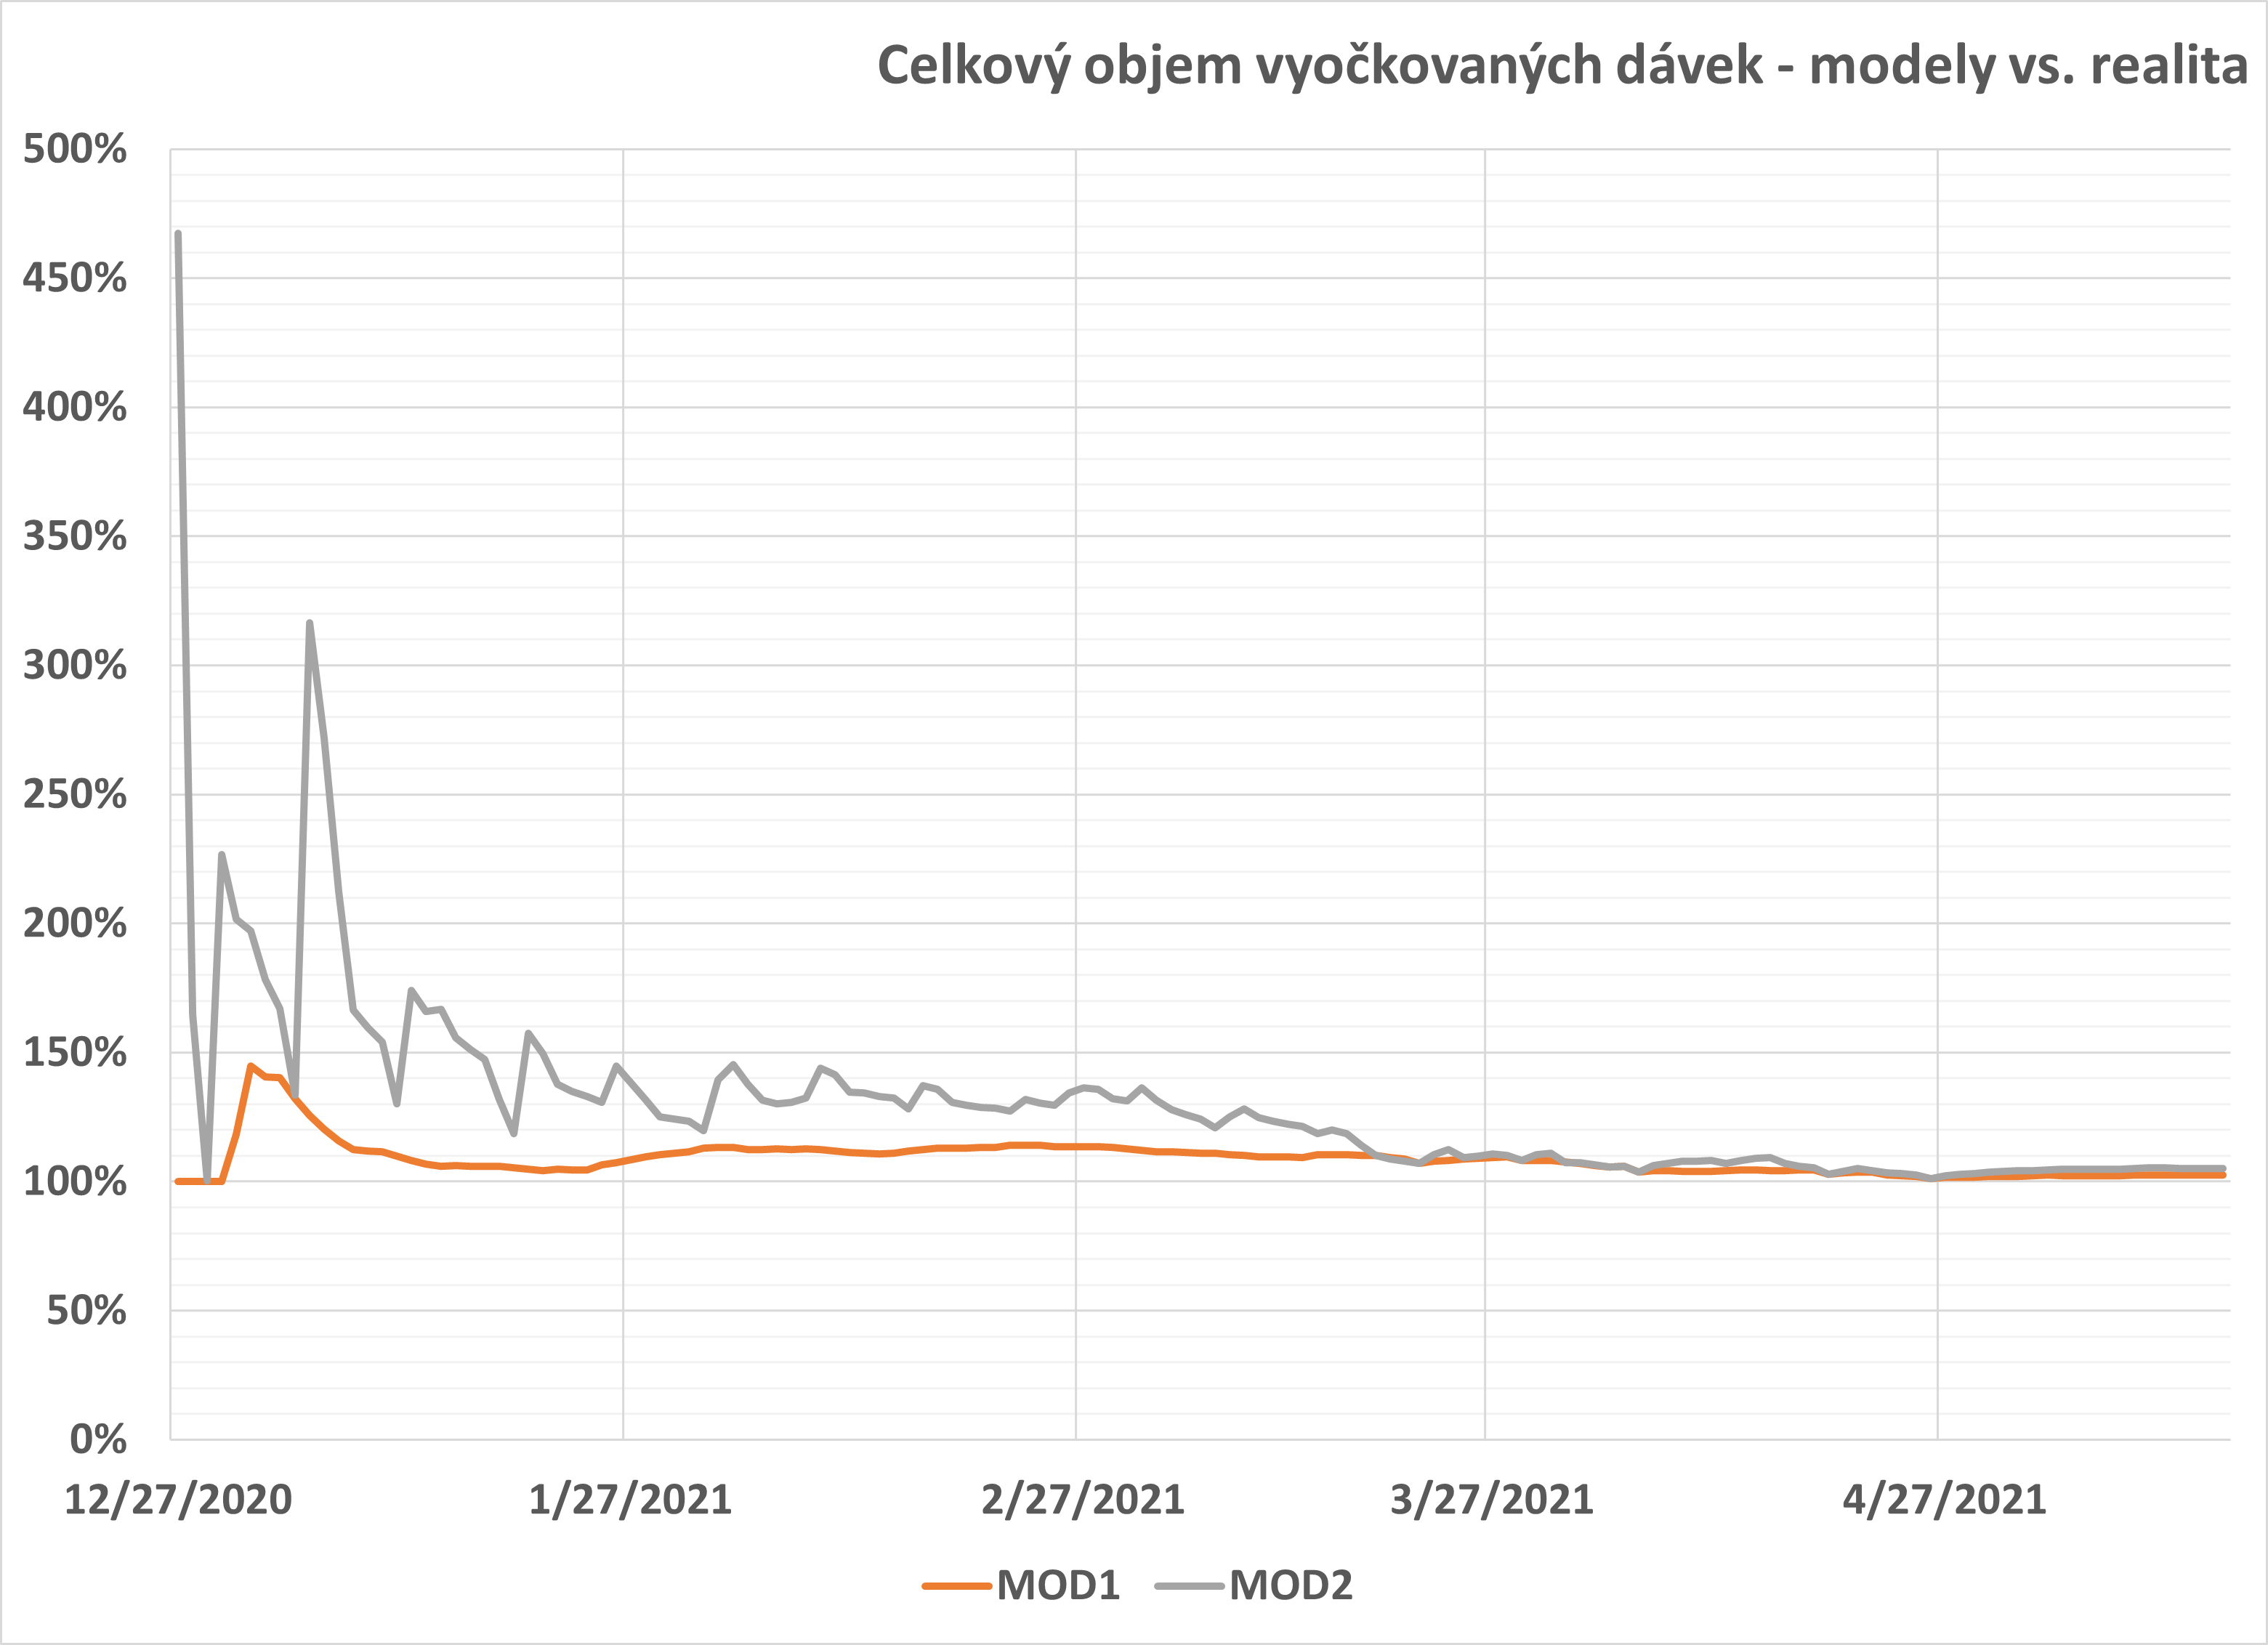
\includegraphics[width=\textwidth]{assets/modely_vs_realita}
\caption{Kumulativní objem očkování (\emph{Realita}=100\%)}
\label{gr_models_delta}
\end{subfigure}



\begin{subfigure}{0.45\textwidth}
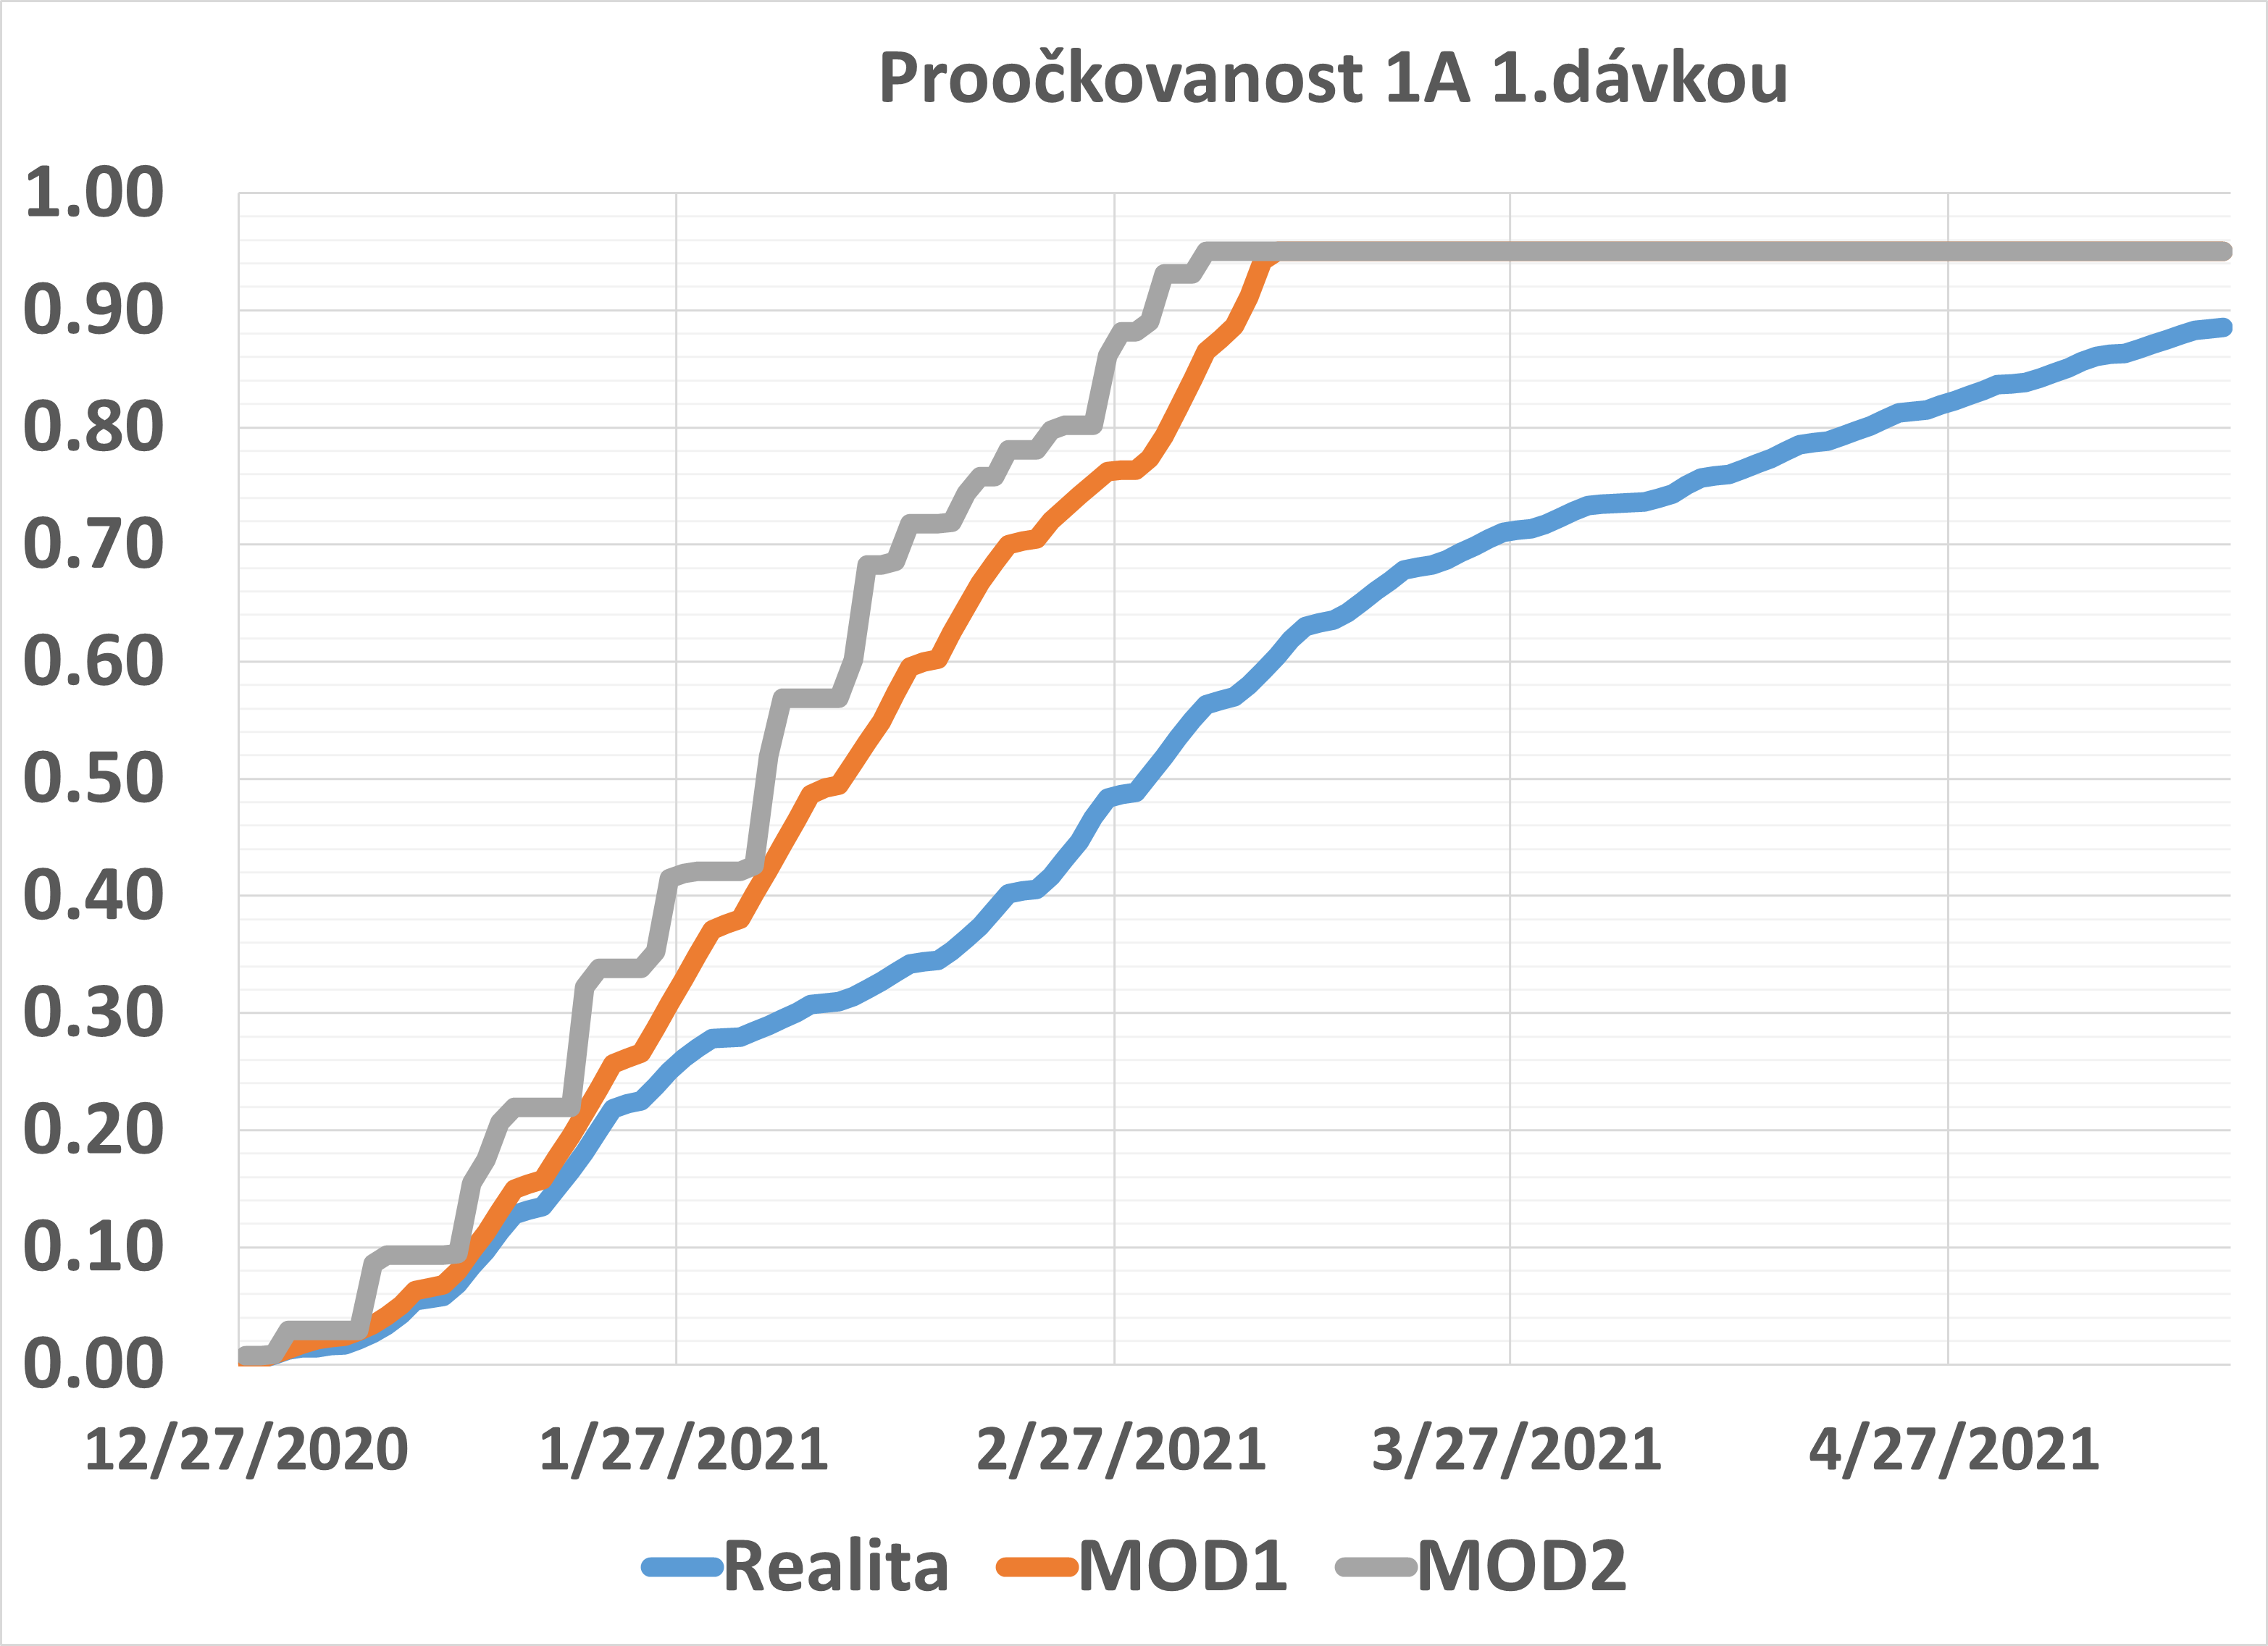
\includegraphics[width=\textwidth]{prispevky/080-Logistika_ockovani/assets/vetsi_popisky/gr_1A_proockovanost}
\caption{Podíl prvních dávek ve skupině I.A}
\label{gr_mod_prvni_davka}
\end{subfigure}
%
\begin{subfigure}{0.45\textwidth}
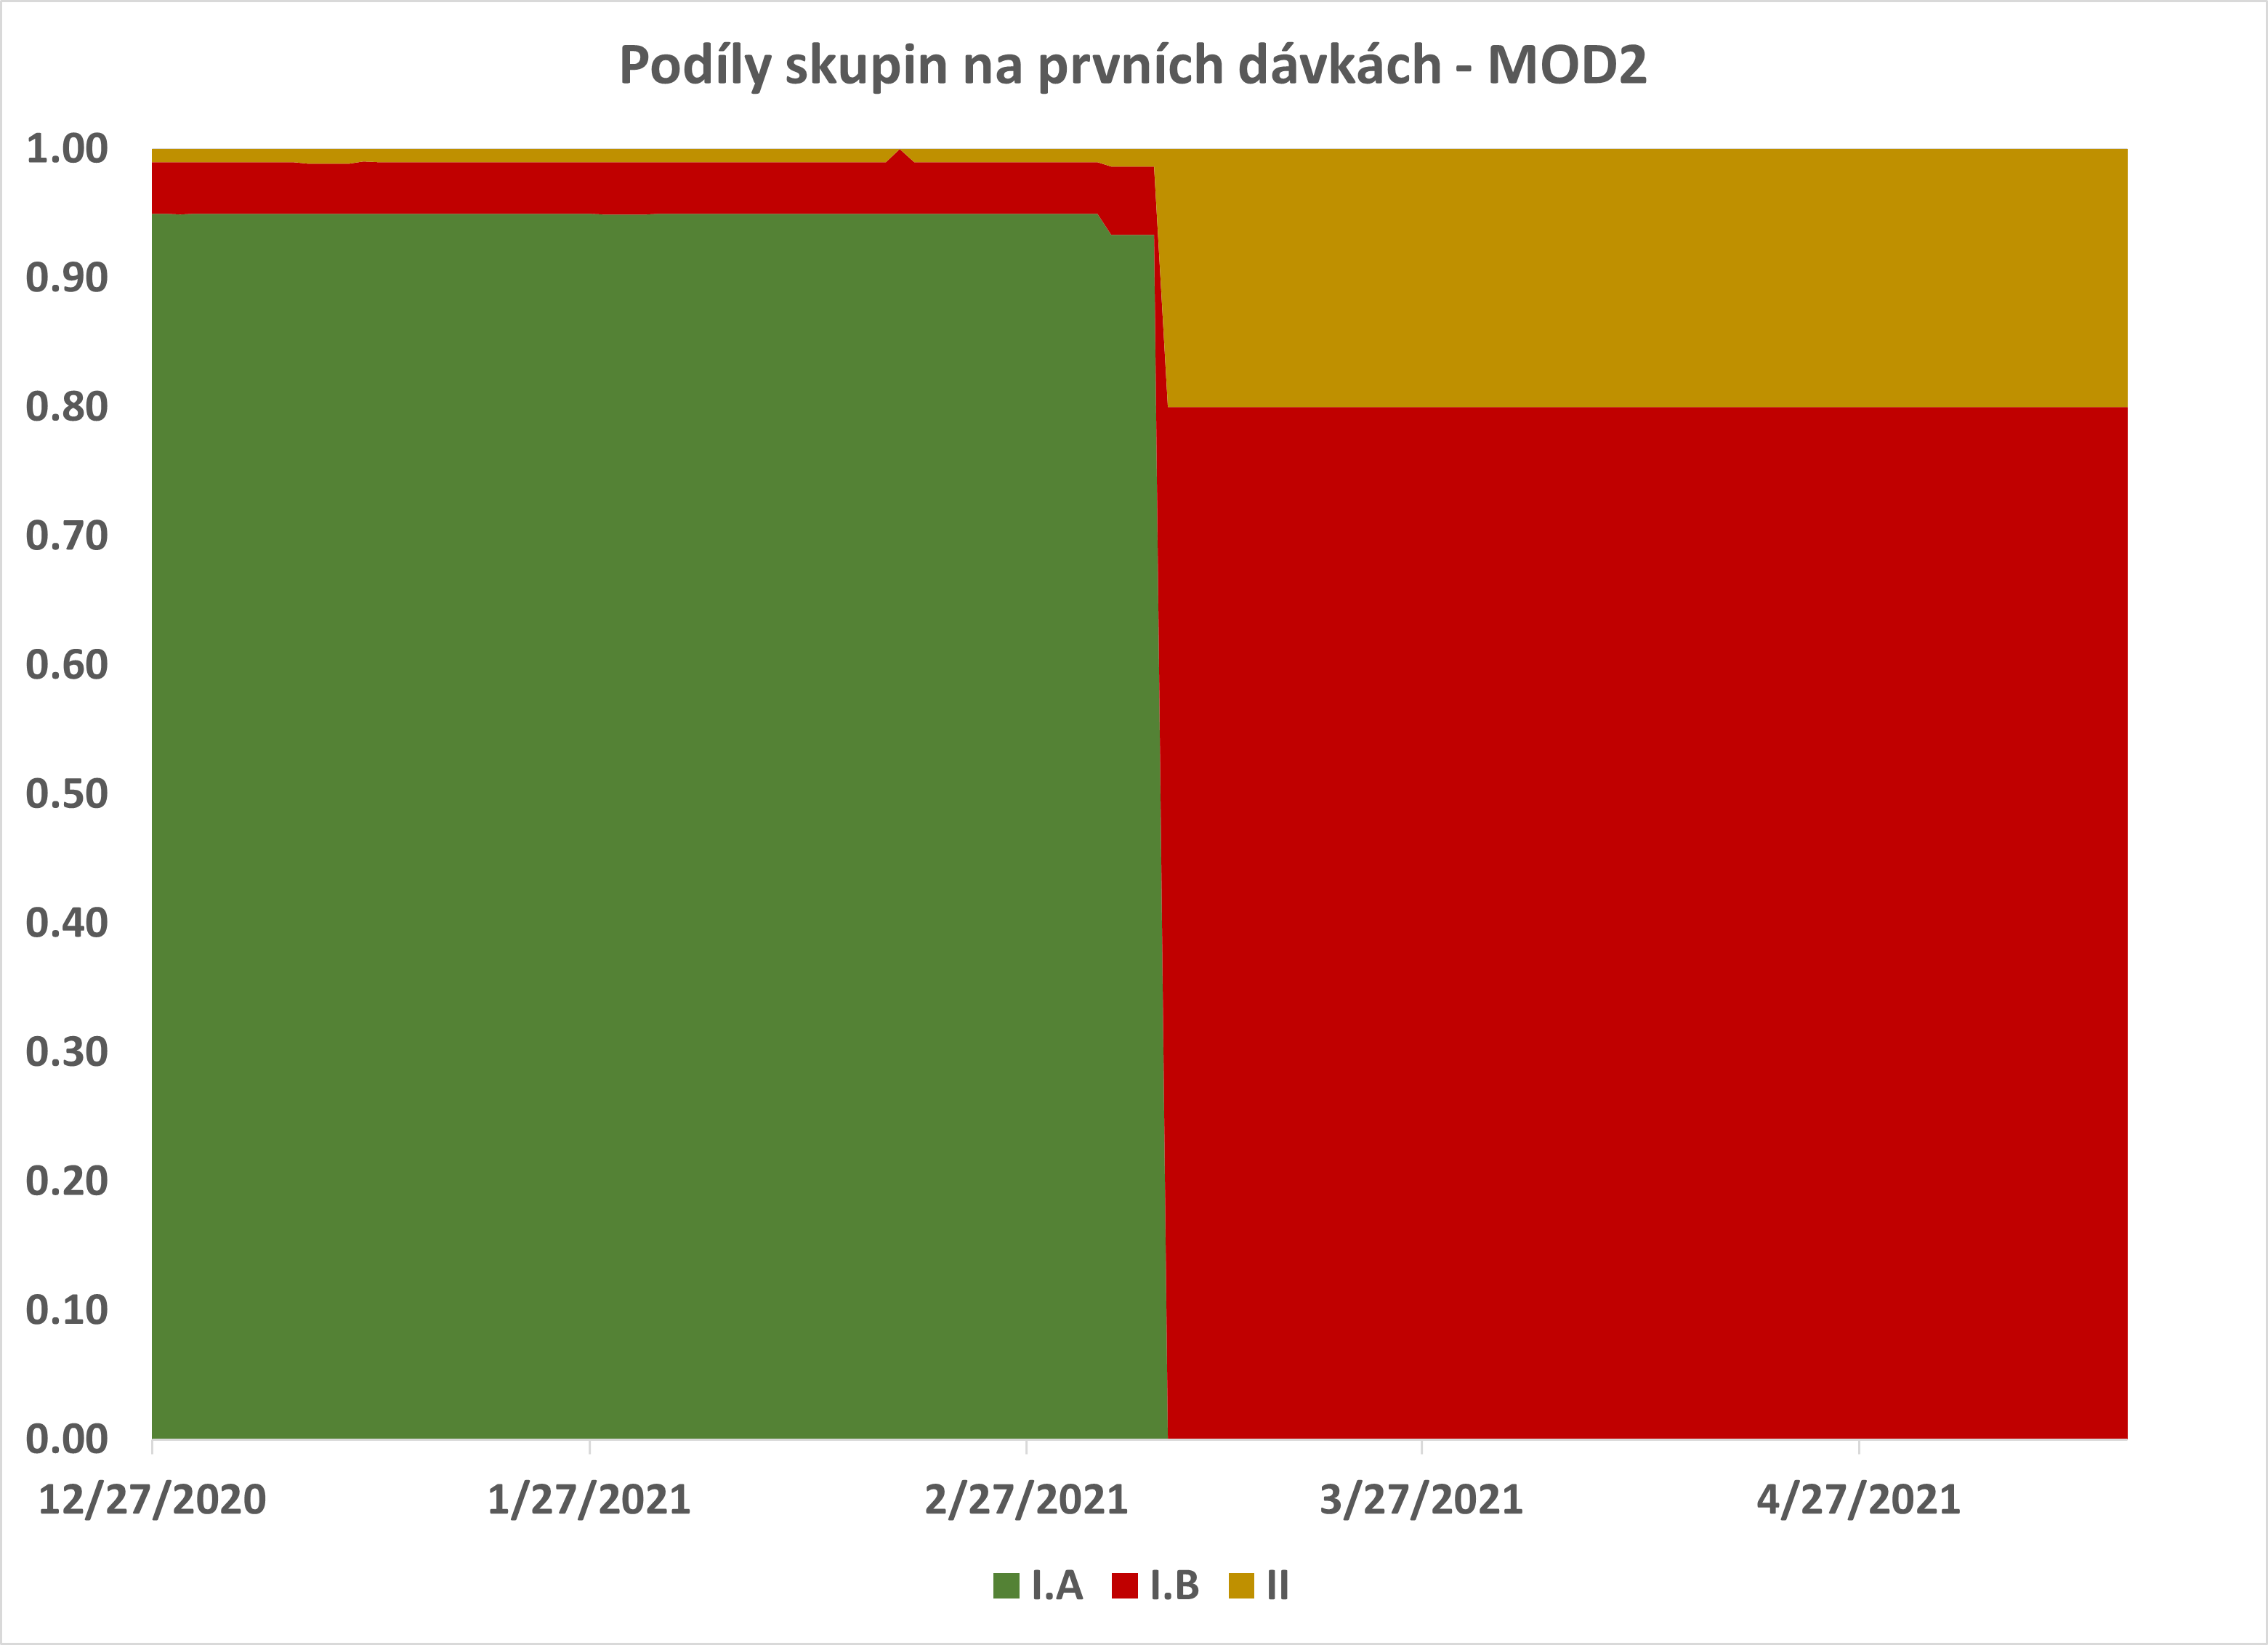
\includegraphics[width=\textwidth]{assets/theta_mod2}
\caption{\emph{MOD2} -- dělení dávek do prioritních skupin nastavených analogicky jako v grafu \ref{gr_real_theta}.}
\label{gr_mod2_theta}
\end{subfigure}

\caption{Dynamika modelovaných scénářů a empirické reality}
\label{gr_modelace}

\end{figure}

\emph{MOD2} je svým nastavením velmi blízký optimálnímu scénáři uvažovanému v sekci \ref{sec_vypocet}. Optimalitu chování tohoto scénáře lze demonstrovat s pomocí dvou grafů. Graf \ref{gr_mod2_theta} zobrazuje striktní prioritizaci dle nastavených kritérií, kde je pro skupinu I.A až do jejího doočkování prvními dávkami držen nastavený podíl $\phi=0,95$ a po jeho ukončení je hodnota $\phi$ pro zbylé dvě skupiny realizována v zadaném poměru $0,04:0,01$. Graf \ref{gr_mod_vyockovanost} ukazuje procentní vývoj vyčerpanosti očkovacích dávek, kde \emph{MOD2} v počátku scénáře udržuje plně vyočkovaný sklad ($1,0$) a v době, kdy začne očkování druhými dávkami (28 dní od začátku běhu scénáře a dále v jeho průběhu) si dle dodávek průběžně udržuje rezervní množství vakcín.

Jak je vidět v rámci grafu \ref{gr_models_delta}, MOD2 byl schopen v úvodních dnech (týdnech) kampaně oproti realitě (100 \% v rámci grafu) významně zvyšovat objem vyočkovaných dávek. \emph{MOD1} dosahuje nižších objemů, avšak postupem času dochází ke konvergenci obou modelů směrem k reálně naměřeným hodnotám. Konvergence je na konci časového období ovlivněna parametrizací modelu\footnote{Hodnota kapacit očkovacích míst $\theta$ je nastavena na maximální kapacity dosažené ke konci sledovaného období.}, nicméně v jeho počátcích je na něm vidět, jaký náskok bylo hypoteticky možné získat udržováním dosažených kapacit (\emph{MOD1}), respektive započetím celého procesu s velkou kapacitou očkovacích míst (vysokou hodnotou $\theta$).

\emph{MOD1} i \emph{MOD2} tak v porovnání s \emph{Realitou} ($4 147 719$ dávek k 16. 5. 2021) dosáhnou vyočkování většího množství dávek ($4 256 776$ v případě \emph{MOD1}, $4 357 846$ v \emph{MOD2}). Kromě vyšší rychlosti v počátečních fázích je klíčovým rozdílem mezi dynamikou hypotetického a reálného světa také důslednost prioritizace. Ta je vedle již popisovaného grafu \ref{gr_mod2_theta} patrná také z grafu \ref{gr_mod_vyockovanost} zobrazujícího podíl vyočkovaných 1. dávek v rámci skupiny I.A. Křivky nárůstu proočkovanosti jsou oproti realitě významně strmější a ve strategii cílovaných 70 \% by s nastaveným intervalem bylo dosaženo pro jednu dávku v rámci února a pro dvě v rámci března. V modelu uvažovaného cíle 90 \% je dosaženo na začátku března, zatímco \emph{Realita} se mu přibližuje až o dva a půl měsíce později. Klesající podíl skladovaných dávek na celku je zaznamenán též v realitu popisujícím grafu \ref{gr_vyuziti}.


Na základě provedené analýzy pokládáme za nejdůležitější dvě zjištění;
\begin{enumerate}
\item I na základě poměrně jednoduchého předpokladu spočívajícího v nikdy neklesajících kapacitách očkovacích míst (\emph{MOD1}) lze v modelovaném světě navyšovat proočkovanost skupiny 1.A významně rychleji, než se tomu dělo v reálném světě (viz zejména  \ref{gr_mod_prvni_davka}). V tomto kontextu dává smysl se ptát, zda by v případě reálného proběhnutí očkování (nejrizikovější) skupiny 1.A bylo možné ušetřit dodatečné životy a kolik lidských životů by tak bylo možné zachránit.
\item Náběh očkovací kampaně byl pomalý nejen co do proočkovanosti 1.A, ale i podílu využitých versus skladovaných dávek (\ref{gr_mod_vyockovanost}). Dostupných dávek tedy tehdy bylo více než pacientů připravených nechat se očkovat. Otázka je, zda mohl stát (například formou dřívější přípravy kampaně) zajistit, aby čekajících (připravených) pacientů bylo ideálně stejně či více než dostupných vakcín.
\end{enumerate}
Faktory potenciálně stojící za dvěma zjištěními dále rozebíráme v následujících sekcích textu.


%Ve Strategii očkování \cite{strategie_covid} je definován cíl co nejrychlejšího proočkování skupin ohrožených těžkým průběhem nemoci, respektive úmrtím. Postup prioritizace jednotlivých skupin obyvatelstva a operační aspekty jsou na high-level úrovni popsány taktéž, dále také v Metodickém pokynu \cite{ockovani_mp}. Rozbor jednotlivých aspektů původního záměru, praktické realizace a míře přiblížení se možnému je poskytnut v rámci jednotlivých bloků této sekce textu. Důraz je kladen postupně na prioritizaci, logistiku očkování a práci s informacemi.




\section*{Faktory efektivity kampaně}
\label{sec:shrnuti}

%Na co si dát v očkování dále pozor (průkazy po první dávce). Důraz na proočkování populace patří do jiných článků. Otázka „odložení“ druhé dávky po aplikaci první (závisí na očkování). Nutnost zajištění registrace subjektů k očkování.
%Spekulace
%Limity studie
%Policy implications -- „jak to má stát použít“

Datově-analytická část článku ukázala potenciál pro dodatečnou efektivitu ležící v důsledné prioritizaci a efektivním využívání skladových kapacit. V této sekci se pokusíme z veřejně dostupných informací identifikovat faktory, které mohly mít (a do budoucna budou mít) na efektivitu vazbu. %, poukazujících na prostor, ve kterém jsme se mohli zachovat efektivněji, respektive budeme tak moci učinit při příštích podobných akcích včetně možného podání booster dávek či přeočkování v budoucnu \cite{logoc_preockovani}. 

Zmíněné faktory klasifikačně dělíme do tří vzájemně se ovlivňujících okruhů. První se zaměřuje na prioritizaci, druhý na roli státu a jeho cíle v procesu a třetí na práci s distribuční sítí. %V rámci první z nich rozebíráme realizovaný versus původně plánovaný důraz na prioritizaci, ve druhé řešíme pojetí role státu v rozhodování o naočkování se a ve třetí předpokládanou versus reálnou složitost celého procesu v kontextu situace v České republice a jejího vývoje.
%
Napříč všemi okruhy argumentujeme, že ačkoli má logistika očkování technické aspekty (podrobněji v předcházejících sekcích), vlastní míra úspěšnosti kampaně je z významné části determinována aspekty behaviorálními. Pro každý z uvedených okruhů témat vycházíme z počátečních předpokladů na straně státu definované Strategií a Metodickým pokynem, respektive dostupných informací k reálnému průběhu tohoto programu a z dalších informačních zdrojů.


\paragraph{Přístup k prioritizaci:} Očkovací kampaň pracovala s cílem dosažení proočkovanosti prioritních skupin před růstem proočkovanosti celé populace. Indikátorem nevyužitého potenciálu v této oblasti může být fakt, že k polovině května nebylo dokončeno ani očkování skupiny I.A, byť podle původních předpokladů se tak mělo stát na přelomu února a března \cite{ockovani_mp}.

%Zatímco podle Strategie měli být v očkování důsledně předřazeni členové rizikových skupin (s cílem snížení množství úmrtí/hospitalizací v důsledku onemocnění covid-19), podle implementace a vyjádření představitelů vlády je možné spekulovat o tom, zda reálným cílem nebylo naočkovat co největší počet osob bez ohledu na prioritizaci. 
%Obecný cíl Strategie namířený na nárůst proočkovanosti celé dospělé populace lze obecně hodnotit kladně.

%Pokud bylo pracováno se započetím programu skrze očkování nejrizikovějších skupin jako s klíčovým prostředkem plnění cílů Strategie, lze konstatovat, že směrem ke specifickým potřebám dotčených skupin (a jejich možným znevýhodněním objektivně bránícím přístupu k vakcinacím) bylo možné udělat podstatně více a dosáhnout vyšší proočkovanosti v kratším čase, jak se stalo v jiných evropských zemích \cite{logoc_vacctracker}. 

Jak je patrné v analytické části, prioritní skupiny byly v období podle Strategie reálně upřednostňovány (tvořily majoritu očkovaných). Vakcíny byly (v některých momentech i prioritizaci navzdory) současně využívány i pro jiné skupiny obyvatel. K tomuto docházelo zejména ze tří důvodů;
%

\begin{enumerate}
\item Vakcín byl v očkovacích místech dostatek, ale členové kritických skupin nebyli registrováni/nepřišli/nevěděli o aktuální možnosti vakcinace v daném místě \cite{logo_nahoda, lochar_karban} 
\item Změny v prioritách na úrovni státu či místních celků \cite{logo_logistika, logo_pardubice}
\item Absence kontrolního mechanismu či tlaku na dodržování prioritizace \cite{logo_predbihani, lochar_karban}
\end{enumerate}


Za prvním důvodem lze identifikovat praktické hledisko fungování procesu registrace a rezervace.
%tím, že byl program realizován bez hlubší přípravy a pečlivého zhodnocení kroků potřebných k naočkování klíčových skupin. 
Rezervační systém měl v období po svém spuštění technické problémy \cite{logoc_seniori_zapsani, logoc_stres}, které se později opakovaly také u nižších věkových skupin. 
Vedle toho se v začátku počítalo například s tím, že se lidé z nejstarších věkových skupin zaregistrují přes internet, což pro řadu z nich nebylo bez asistence prakticky možné \cite{seniori_registrace_internet}.
%Vedle toho se v počátcích pří nemyslelo na jeho přizpůsobení potřebám nejstarších skupin obyvatel,
%
%, pro něž bez asistence prakticky přístupný nebyl. 
Jako možná prevence komplikací při práci se systémem by se nabízelo například otevření registrace již v době před doručením očkovacích dávek (například v prosinci 2020), čímž by se případné problémy mohly odlaďovat v klidnějším nastavení. % Všichni předmětní aktéři (očkovací centra, očkovaní, pomocný personál) se mohli nachystat na konkrétní časy očkování, respektive objemy potřebné práce. 
Současně by tak bylo možné dát veřejnosti jasné signály o tom, co a jak bude v brzké době probíhat.

Druhý důvod, předřazování jiných skupin, lze do určité míry vnímat jako logický dopad nízké účasti nejohroženějších skupin v prvních fázích kampaně.
%
%Zmiňované obtíže, které byly nejviditelnější v počátcích očkovacího programu, byť v různé míře intenzity přetrvávaly dlouhodobě, vedly k tomu, že byl volný prostor vyplňován očkováním jiných skupin obyvatel, nikoli nejohroženějšími seniory, kteří naráželi na bariéry v dostupnosti vakcinace \cite{seniori_registrace_internet}. 
Ve všeobecnou známost vstoupil případ naočkování 1000 zaměstnanců Státního zdravotního ústavu a jejich příbuzných či očkování jednotek dobrovolných hasičů v pražských částech Suchdol a Lysolaje \cite{logoc_nebudu, logoc_hasici}. Je na zvážení, zda bylo u některých ze jmenovaných skupin zařazení do prioritizace skutečně oprávněné, nicméně svévolné úpravy mohou signalizovat, že se očkovací místa dostala poměrně záhy mimo pole, ve kterém plánování probíhalo, a v podstatě improvizovala. 

Třetí bod směřuje k absenci aplikace mechanismů, jež by odklonům od prioritizačního plánu dokázaly zabránit.
%Ačkoli zde existovala prioritizace podle věku, prakticky dodržována nebyla, respektive neexistoval zde reálný tlak na vymáhání takto nastavených pravidel. Opakovaně tak docházelo k případům, kdy byli očkováni lidé či skupiny lidí zcela mimo registrační systém a bez jakékoli reálné priority \cite{logo_hejtman, logo_predbihani}. 

Vedle zmiňované reprioritizace skupin se do systému dostávali i vybraní jednotlivci \cite{logoc_namestkyne, logoc_kabatek, CTK2021JsemDenik, logo_hejtman, logo_predbihani}.
Tímto způsobem mohl ze strany veřejnosti vzniknout dojem, že vakcíny jsou dostupné pro ty, kteří si přístup k nim \emph{umějí zařídit}. 

Nedodržování prioritizace nahrávala i počáteční nejistota týkající se dodávek, omezená doba použitelnosti vakcín a také skutečnost, že první vakcinační centra vznikala v nemocnicích, které v té době čelily přílivu velkého množství pacientů s covid-19 a současně musely řešit logistiku očkovacího programu, ačkoli se dostávaly na hranice možností svých personálních i provozních kapacit. 


%Zejména v počátečních fázích kampaně tak dodávky vakcín nebyly efektivně využívány a jednotlivé dávky byly aplikovány nahodile. Pravděpodobně tak bylo možné zabránit většímu množství úmrtí, pokud by byla dodržena nutná prioritizace \cite{blog_ucitele}. 
%Doposud nevznikl státem garantovaný veřejně dostupný informační systém, v němž by občané mohli najít informace o tom, jak dalece „plynulý“ je provoz v jednotlivých očkovacích místech. Stejně tak neexistuje možnost určit svou preferenci, například v určité vzdálenosti či zvolit při registraci více očkovacích míst, aby následně byl člověk přiřazen k tomu, kde získá nejdřívější termín. V rámci registračního systému vznikala místa, kde je značný převis poptávky nad nabídkou volných termínů, a naopak jiná místa dostatečně nevyužívají své kapacity včetně dodávaných vakcín. V tomto ohledu vznikla soukromá iniciativa Laboratoře otevřených dat při Fakultě informačních technologií ČVUT \cite{logoc_ockoweb}, která umožnila se zpožděním maximálně 24 hodin sledovat, kolik osob čeká v daném očkovacím místě na rezervaci termínu i jak plynule je zde očkování odbavováno. Další jednorázovou iniciativou, jejímž cílem bylo zpřístupnit očkování těm, kteří čekají na volný termín, byl očkovací maraton probíhající v několika očkovacích centrech ve Středočeském kraji \cite{logoc_maraton}, kdy se mohli zájemci nechat očkovat i bez předchozí registrace. 
 
\paragraph{Role a cíle státu v procesu:} Role, kterou v rámci kampaně sám sobě určil stát, je do značné míry propojená s rolí občanů jako subjektů očkování. Stát deklaroval možnost nesplnění cílové proočkovanosti prioritních skupin v případě nedostatečného zájmu veřejnosti \cite{kdoprvni}. Komunikace vládních představitelů se tak soustředila zejména na úspěchy v podobě toho, kolik vakcín bylo kam dodáno, jaký další objem očkovacích látek do země dorazí či jak co nejefektivněji využít velkokapacitní centra i za cenu, že lidé budou za očkováním dobrovolně cestovat \cite{babis_echo}.

Z řečeného lze usuzovat, že ani osoby odpovědné za očkovací kampaň neměly proočkovanost nejrizikovějších skupin mezi svými definovanými cíly pro hodnocení úspěšnosti celé akce. Tento faktor dohromady 
se spuštěním komunikační kampaně až takřka pět měsíců po zahájení očkování \cite{logoc_naruby,logoc_zpozdeni} vytváří situaci, kdy s nejrizikovějšími skupinami není pracováno v rovině přesvědčování ani informování, a tyto skupiny jsou tak v rozhodování o (ne)naočkování se odkázány jen na své dosavadní znalosti a informace, které se k nim dostanou od jiných aktérů než od státu. Důraz kladený na provedení kampaně ze strany státu se odráží i v tom, že na vedení celé kampaně byl v počátku najat koordinátor pouze na částečný úvazek, a to pouze několik týdnů před vlastním zahájením očkovacího programu, a následně tuto funkci vedle řady svých dalších povinností vykonával sám premiér \cite{ocko_blahuta,babis_koordinator}. %Poté, co funkci dobrovolně opustil, převzal tuto funkci sám na sebe premiér \cite{babis_koordinator}. Vývoj situace budí dojem, že premiér k očkovacímu programu přistupoval v rámci svého mikromanagementu obchodního artiklu, jejž stačí nabídnout a veřejnost se přihlásí sama \cite{ocko_respekt}. Ve Strategii očkování tak například není prakticky zvažována otázka motivace veřejnosti k očkování ani možné bariéry, které by mohly bránit úspěšné participaci občanů na očkovacím programu \cite{logoc_skvrny}. Zcela chyběl náhled, že realizaci očkovacího programu ovlivňuje řada behaviorálních faktorů \cite{duvody_zd}.









%což lze interpretovat také tak, že stát se sám zříká zodpovědnosti za naplnění této strategie, respektive se na jejím naplnění podílí jen omezeně. 

%Oficiální komunikační kampaň k očkování proti covid-19 spustilo ministerstvo zdravotnictví v polovině dubna 2021, tedy téměř pět měsíců po zahájení očkovací kampaně. 
%Podle opakovaných vyjádření úřadu a také premiéra se tak stalo proto, že by dřívější zahájení kampaně nemělo požadovaný efekt, případně by vedlo k nerealistickému očekávání o dostupnosti očkování v době, kdy byly dodávky vakcín velmi limitované a v rámci regionů nestabilní \cite{logoc_tlak}. 

%Český očkovací program podle našeho názoru byl a dosud je primárně postaven na tom, že občané sami aktivně vyjádří svůj zájem o očkování a budou i bez vnějších incentiv ochotni učinit konkrétní kroky i za cenu jistého nepohodlí pro to, aby vakcinace dosáhli. 
Lze vznést otázku, zda se výchozím předpokladem nestalo, že občané o očkování stojí a stát by měl být jen jakýmsi servisním střediskem, které zajistí potřebné dodávky očkovacích látek a již neřeší motivaci občanů k očkování, přístup k němu \cite{logoc_zpozdeni} či překážky týkající se specifických skupin v rámci společnosti \cite{logoc_skvrny,logoc_romove}. %Zdá se, se stát bohužel nepracoval s variantou, že pro část populace bude očkování z objektivních důvodů nedostupné, respektive bude spojeno s významnými překážkami \cite{logoc_skvrny,logoc_romove}. Vznikla tak řada „bílých míst“, tedy skupin osob, které propadly očkovacím systémem. 
Jednou ze skupin vyžadujících osobnější přístup mohou být samostatně žijící senioři nad 80 let, kteří naráželi na obtížně překonatelné problémy s registrací, někteří z nich dlouhou dobu čekali na možnost nechat se očkovat u praktických lékařů a k 16. květnu 2021 jsou nejméně proočkovanou podskupinou v rámci I.A. Tato skupina je dále specifická tím, že jsou její členové na rozdíl například od zdravotníků či osob v institucionalizované péči prostorově rozptýleni. Pokud se stát snažil maximalizovat celkovou proočkovanost namísto proočkovanosti prioritních skupin, bylo pro něj racionální pracovat spíše se skupinami, které je možné snadno shromáždit na jedno místo a očkovat po desítkách \cite{blog_ucitele}.  
%Cíl v podobě maximalizace celkové proočkovanosti je tak pro státního plánovače u této skupiny obtížněji dosažitelný.








%\subsection*{Co bylo cílem vlády?}
%Spoléhat se v otázce očkování na dobrovolnou motivaci občanů však má svá úskalí, zejména v případě, kdy veřejnost není dostatečně přesvědčena ke spolupráci. 
%Základním předpokladem by měla být dostatečná informovanost o benefitech očkování jak pro jednotlivce, tak pro celou společnost, aby se veřejnost mohla zodpovědně rozhodnout. Nelze opomenout skutečnost, že se očkovací program rozběhl v době, kdy byla česká společnost pod značným vlivem dezinformací, které ovlivňovaly i vnímání pandemie i vakcinace jako takové \cite{logoc_stem}. Lze konstatovat, že v tomto ohledu bohužel vláda prohrála boj s dezinformacemi, respektive předem vyklidila pole \cite{logoc_eh}. 

Problém doručení informací či vakcín (pro stát) těžce oslovitelným skupinám může být řešitelný například skrze úzkou spolupráci mezi státem a neziskovým sektorem, který s řadou skupin dlouhodobě pracuje a má jejich důvěru \cite{logoc_bilamista}. Neziskové organizace byly zapojeny již od počátku kampaně, a to na základě vlastní iniciativy „zdola“, v jejímž rámci zajišťovaly registrace svých klientů k očkování \cite{ocko_ngo}. Iniciativu také často přebíraly samosprávy a také jednotlivé kraje, které v rámci svých kompetencí hledaly možnosti, jak očkování co nejvíce zpřístupnit, a to zejména nejohroženějším skupinám populace. 

%Doposud nebyla systematicky analyzována role neziskového sektoru v rámci očkovacího programu. Jedním z důvodů může být skutečnost, že při plánování strategie se s ním nepočítalo, byť reálně byly neziskové organizace zapojeny již od počátku očkovacího programu, a to na základě vlastní iniciativy „zdola“ ze strany samotných organizací  \cite{ocko_ng}. Zapojení neziskového sektoru je nástroj, který reálně odstraňuje bariéry v přístupu k vakcinaci \cite{logoc_bilamista}. Tyto organizace sehrály důležitou úlohu při vstupu svých klientů do očkovacího systému. Přesněji, pokud byla součástí jejich služeb asistence klientům například při kontaktu s úřady, stala se asistence při registraci do očkovacího systému náplní jejich práce. Jejich pracovníci a pracovnice také pravděpodobně byli zdrojem informací o očkování pro své klienty, mimo jiné proto, že s nimi dlouhodobě pracují a mají jejich důvěru.



\paragraph{Práce s distribuční sítí:} Jak je vidět již na grafu \ref{gr_vyuziti_zrizovatele}, zřizovatelé z řad soukromých fyzických a právnických osob jsou v podílu vyočkovaných dávek výrazně za státem a nižšími správními celky. Většina objemu vakcín tak byla ve sledovaném období aplikována ve velkokapacitních očkovacích centrech.% postaven na velkokapacitních očkovacích centrech, kam také primárně směřují dodávky vakcín. %Existence těchto center umožňuje vakcinaci velkého počtu osob v krátkém čase, avšak tato centra neodpovídají potřebám celé dospělé populace, a pro část mohou být dokonce důvodem, proč není vakcinována. 

%V rámci očkovací strategie i její následné realizace byla ze strany státu zcela opomenuta role neziskového sektoru, který však během vlastní kampaně dokázal vyvinout řadu iniciativ odstraňujících bariéry v přístupu k vakcinaci zejména seniorů. Klíčovou roli tyto iniciativy, na nichž se podílely také některé samosprávy, sehrály při vstupu do registračního systému. Je možné, že část seniorů mohla očekávat, že budou aktivně osloveni, například ze strany své zdravotní pojišťovny či praktického lékaře, a pokud se tomu tak nestalo, mohli podlehnout dojmu, že se jich očkování (ještě) netýká. V tomto ohledu lze skutečnost, že nedošlo k systematickému aktivnímu a cílenému oslovování nejohroženější části populace ze strany státu/veřejných institucí, vnímat jako promarněnou příležitost (podrobněji psychologická kapitola sborníku). 


%Podle původních předpokladů definovaných v rámci Strategie očkování ministerstva zdravotnictví měli být paradoxně právě praktičtí lékaři tím, kdo bude páteří očkovacího systému. Podle tohoto materiálu měli praktičtí lékaři očkovat 50 tisíc osob denně: „Tato kapacita (pozn. redakce -- odhadované množství očkovaných v ordinacích praktických lékařů) umožní, aby bylo očkování nabídnuto všem, kteří o něj budou mít zájem,“ konstatuje dokument.  

Původní strategie očkování počítala s očkováním až 50 tisíc osob denně v ordinacích praktických lékařů, jakmile to bude umožněno dostupností vakcín Astra Zeneca a Janssen\footnote{Resp. zavážení dávkami vakcíny Moderna z velkých balení skladovaných ve velkokapacitních centrech.} \cite{strategie_covid}. Po opětovném posouzení ze strany Evropské lékové agentury došlo v polovině května 2021 ke změnám doporučených podmínek pro distribuci a skladování nejvíce zastoupené vakcíny Comirnaty \cite{logoc_pfizer_mrazak}, čímž se i pro tuto vakcínu teoreticky otevřela možnost očkování v rámci menších zdravotnických zařízení a ordinací praktických lékařů. %Vznikla tak další kapacita pro očkování, jež není nyní plně využívána. 
Praktičtí lékaři opakovaně deklarovali, že jsou na očkování připraveni, a dožadovali se možnosti ho realizovat \cite{logoc_svl,logoc_pripravenost}, opakovaně však naráželi na nedostatek očkovacích látek způsobený zejména problémy v oblasti distribuce a logistiky vakcín, což vedlo k tomu, že své pacienty museli odmítat či sami v rámci omezeného množství dávek prioritizovat zájemce podle jejich věku, případně zdravotního stavu \cite{logo_logistika}. 
%
%Společnost všeobecného lékařství ČLS JEP stejně jako Sdružení praktických lékařů a organizace Mladí praktici opakovaně deklarovali připravenost a ochotu očkovat své pacienty \cite{logoc_svl,logoc_pripravenost}. %Jako zástupci primární péče jim jsou nejblíže, a to mnohdy místně i časově, mají jejich důvěru a současně jsou vnímáni jako někdo, kdo je schopen adekvátně posoudit zdravotní stav jedince vzhledem k vakcinaci. To také vedlo k tomu, že se řada osob zejména vyššího věku registrovala do ordinací svých praktických lékařů a ani nezvažovala možnost využití některého z velkokapacitních center. 
Podle informací od praktických lékařů však v mezičase klesl zájem pacientů o očkování v jejich ordinacích, respektive ti, kteří se chtěli nechat očkovat, již tak učinili v očkovacích centrech \cite{logo_praktici}. 
%
%To vedlo a stále spolu s dalšími body praktické realizace očkovací strategie vede ke konkrétním nepříznivým důsledkům, kdy stále není ukončeno očkování seniorů v kategorii 65+, respektive ani v nejohroženější skupině 80+. 
Chybějící kapacita praktických lékařů se projevila i na celkovém objemu provedených očkování. Navzdory deklaraci premiéra z poloviny března 2021, že na začátku dubna již bude očkováno 100 tisíc osob denně \cite{logoc_100k}, se tuto hranici podařilo překonat až na konci května \cite{logoc_100kmame}. %Současně již nedochází k výraznému nárůstu proočkovanosti v nejstarších věkových skupinách, což potenciálně znamená, že se nepodaří zabránit nutnosti hospitalizace a případně úmrtím, jimž by bylo možné předejít očkováním.




%\subsection*{Data a systémy -- zatím nevyužitý potenciál}
%Vedle již řečeného je dále možné spekulovat o tom, zda stát nehledá velké koherentní skupiny proto, že to je analytická úroveň, kterou jeho současní představitelé zvládají. Tento argument by mohl být podpořen identifikovanými sklony premiéra Babiše k mikromanagementu, tedy stylu řízení, v jehož rámci se manažer snaží osobně řídit větší skupinu přímých podřízených. Konkrétním příkladem může být mimo jiné to, že se osobně prezentoval jako někdo, kdo počítá dodávky vakcín \cite{ocko_pocita}. Úspěch v cílené identifikaci malých skupin či jednotlivců může přitom být naopak závislý na delegování problému na lokálně působící neziskové organizace či městské úřady.

%Strategie očkování v Česku vznikala ve srovnání s jinými zeměmi se zpožděním a byla dokončena prakticky několik dnů před spuštěním očkovacího programu, respektive před dodáním prvních vakcín \cite{strategie_idnes}. 

%Míru připravenosti státu na plánování na základě analýzy dat ukazuje také datová kvalita veřejně poskytovaných zdrojů. V datech od státu například aktuálně (v polovině roku 2021) zcela chybějí vakcíny Janssen a z dat o rezervacích není možné rekonstruovat hodnoty, ke kterým představitelé vlády docházejí ve svých prezentacích.

%Tento problém souvisí v konečném důsledku s ontologií světa, v jehož rámci vláda funguje. Pokud byla tématem jara 2020 exponenciální křivka růstu incidence a na podzim 2020 jsme viděli dopad zpožděného zavedení opatření, bylo by od vlády namístě chtít, aby byla schopná očkování provést tak, že jeho výsledky nejsou postaveny jen na kumulativní proočkovanosti populace (jakkoli je důležitá), ale zejména na pokrytí nejrizikovějších skupin.


%\subsection*{Výhledy pro další měsíce}

%Konkrétní snahou vlády s cílem motivovat veřejnost pro očkování byla na konci května 2021 změna pravidel pro očkované osoby. Pokud byla podána alespoň jedna dávka vakcíny (v případě dvoudávkového očkovacího schématu) a od podání první dávky uplynulo více než 21 dnů, bylo na tyto osoby nahlíženo jako na očkované a již se na ně nevztahovala povinnost testování. Toto rozhodnutí vlády padlo i přes nesouhlas České vakcinologické společnosti ČLS JEP, která upozorňovala na skutečnost \cite{logoc_certifikat}, že pouze ukončené očkování (alespoň 14 dnů po podání druhé dávky vakcíny v případě dvoudávkového schématu či po podání vakcín v jednodávkovém schématu) zajišťuje potřebnou ochranu před nákazou. Někteří částečně očkovaní jedinci mohou pod vlivem skutečnosti, že je s nimi nakládáno stejně, jako kdyby byli plně očkováni, podlehnout falešnému pocitu bezpečí, že již jedna dávka poskytuje potřebnou ochranu před nákazou, a změnit podle toho své chování a tím zvýšit riziko nákazy. Dalším rizikem je, že se část takto částečně očkovaných již nedostaví na druhou dávku, protože jim z jejich pohledu již nemusí přinést potřebné výhody, respektive ke zjednodušení jejich každodenního života již došlo. Současně lze považovat za problematické, že se minimálně z pohledu komunikace vládních představitelů změnil dlouhodobý cíl očkovací kampaně z dosažení potřebné imunizace celé populace na krátkodobé zjednodušení běžného života. 

%Nicméně na základě politického rozhodnutí došlo ke změně, kdy částečně očkovaní po uplynutí třítýdenní lhůty nemusí podstupovat testování před využíváním některých služeb ani při cestách z/do některých jiných států. Tato změna pravidel však platila pouze do začátku července 2021, kdy došlo k návratu k původnímu stavu, tedy že pouze plně očkované osoby již nemusí podstupovat testování \cite{ocko_davka}. Důvodem k tomuto kroku byly obavy, že v případě opětovného zhoršení epidemiologické situace zde nebude dosaženo potřebné úrovně proočkovanosti a současně zde mohou vzniknout ohniska infekce (podrobněji kapitola sborníku Šmíd). 




%Zpožděná kampaň byla skutečně spuštěna v době dostatečných dodávek vakcín, avšak pokud bychom předpokládali, že se její efekt projeví s časovým odstupem, je zde riziko, že její účinnost bude brzy snižována souběžnými informacemi o poklesu denních počtů očkovaných (respektive nevyužívání dostupného objemu dávek). Současně toto zpoždění znamenalo, že veřejnost se několik měsíců pohybovala v oficiálním informačním vakuu, a o to zranitelnější byla vůči zavádějícím informacím nebo přímo dezinformacím, což mohlo ovlivnit následné rozhodování o vlastní vakcinaci.



\section*{Závěr}

Celý proces očkovací kampaně lze (do technologické úrovně) matematicky modelovat a naplánovat, což dává prostor k dostatečné přípravě a systematickému plánování na základě dostupných dat a práce s nimi. Funkčnost implementace však bude z velké části ležet v oblasti behaviorálních faktorů, tedy zejména v přesvědčení veřejnosti ke spolupráci na očkovacím programu, jak již ukázaly předchozí měsíce. 
%
Proto je stále zásadní klást důraz na kvalitně zdůvodněnou prioritizaci a také bránit její dodržování v praxi. %Respesktive nastaveným cílem bude, aby se očkovali primárně ti nejohroženější, i s tím, že některé z nich bude nutné cíleně oslovit a proces vakcinace jim přizpůsobit, aby nezůstalo u pouhých proklamací. Mimo jiné to znamená aktivně přistupovat k existenci bariér, které mohou bránit v očkování celým skupinám populace, a ve spolupráci s neziskovým sektorem, který již prokázal svou připravenost a také akceschopnost, pracovat na jejich odstranění. Právě neziskový sektor spolu s místní samosprávou dokáže individuálně zasáhnout „zdola“ jednotlivce, zatímco stát toho ze své podstaty schopen není. 

Je možné, že vzhledem k aktuální situaci v době psaní článku, tedy vývoji epidemiologické situace, výskytu nových variant viru SARS-CoV-2 a také pravděpodobnému poklesu imunitní ochrany po provedené vakcinaci v čase bude namístě zvažovat podání booster dávky vakcíny a případné následné další přeočkování u více skupin populace. %Proto je zcela opodstatněné již nyní zvažovat variantu, že bude nutné upravit očkovací strategii a zvažovat nové či zatím pouze okrajově využívané možnosti pro oslovení prioritních skupin včetně zjednodušení systému registrace \cite{ocko_registrace}. V této souvislosti považujeme za vhodné dále analyzovat data o průběhu očkovací kampaně, zejména s přihlédnutím k jejím „bílým místům“, a současně se předem připravit na tento možný scénář opětovného plošného očkování (přinejmenším rizikových skupin populace), aby jeho následná realizace již byla hladší. 

Ke zvážení je také změna optiky, kdy by vakcinace neměla být vnímána jen jako individuální benefit pro jednotlivé občany, zejména v kontextu nastavení oficiální komunikace státních institucí zdůrazňující očkování jako vstupenku k obnovení ekonomických a volnočasových aktivit, kdy role státu spočívá pouze v zajištění očkovacích látek a očekávání aktivního zájmu občanů, ale rozšíří své působení o další úvahy, kdy bude zdůrazňovat také etické a altruistické aspekty očkování. %To je důležité i pro vnímání zahájení vakcinace věkové kategorie 12 až 15 let, která nepatří mezi rizikové skupiny a vakcinace na osobní úrovni zde přináší omezené benefity ve srovnání s vyššími věkovými kategoriemi. 
Mimo jiné to znamená v komunikaci státu návrat k původnímu \emph{altruistickému} smyslu vakcinace, kdy většinová populace (podstatně méně ohrožená těžkým průběhem onemocnění) svým naočkováním limituje šanci na vznik nové mutace, která by byla schopna obejít imunitu získanou předchozím proděláním nemoci nebo očkováním, či na opětovné rozšíření choroby, tedy přednostně ochránit nejzranitelnější skupiny populace a následně chránit populaci jako celek. 

%V době psaní tohoto článku (červen 2021) očkovací program stále nebyl u konce. Naopak se otevírají nové otázky, které bude třeba zodpovědět, ať už jde o očkování mladistvých, možné očkování dětí či podání booster dávek a následné přeočkování. 

Při přípravě na další měsíce již nemusí jít o zajištění dostatečného množství vakcín, ale spíše právě o přesvědčování dostatečné části populace napříč věkovými skupinami o tom, že se má naočkovat a své očkování také dokončit. Ve srovnání s rokem 2020 tak není klíčovou otázkou logistika, nýbrž spolupráce veřejnosti. Cestou k dosažení spolupráce může být mimo jiné otevřená komunikace a předvídatelné jednání ze strany státu. Příležitostí pro aplikaci závěrů článku může být kromě doočkování zatím neočkovaných také rozbíhající se aplikace třetí, tzv. \emph{booster} dávky u vybraných skupin populace, a případné následné další přeočkování v budoucnu. 





%V rámci této sekce se snažíme definovat optimální očkovací strategii pro inertní svět, tedy zcela bez využití reálného přístupu zvoleného Českou republikou v otázce očkování. Uvažovaný svět má však parametry České republiky mezi podzimem 2020 a jarem 2021 v ostatních aspektech odpovědi na pandemii. Uvažujeme tedy platné rozšíření pandemie mezi obyvatelstvem, státní odpovědí na ni i hraniční vytížeností nemocnic. Dále také pracujeme se známými informacemi o samotné pandemii, zahrnujícími zejména exponenciální závislosti mezi časem a nárůstem nakaženosti obyvatelstva při neplatnosti protiepidemických opatření a mezi věkem nakaženého a úmrtností na onemocnění.


%Tento cíl lze realizovat buď přímo (naočkujeme člena rizikové skupiny), nebo nepřímo (naočkujeme pracovníka klíčového pro záchranu životů, například lékaře).
%Úloha má řadu vzájemně provázaných aspektů, jež je nutné v rovině parametrů, proměnných či omezení zohlednit. V rámci této úvahy pracujeme se čtyřmi oblastmi
%\begin{enumerate}
%\item Doručení dávek optimálním příjemcům (prioritní skupiny, registrace)
%\item Plánování dávek v čase (nechodí najednou, musíme rozdělit na první a druhou) (očkovací místa a jejich kapacita, role PL, mezinárodní logistika i logistika na cílový bod, mrazení a odmrazování) 
%%\item Plánování dávek v prostoru 
%\item Informační toky (co by mělo vědět očkovací místo, občané...).
%\end{enumerate}
%%Každá ze zmíněných oblastí je nyní do větší podrobnosti rozebrána v samostatné podsekci. 
%%Může být složitější
%%
%Ve zbytku této sekce je do podrobnosti rozepsáno, jakým způsobem lze (při dostupných informacích) jednotlivé z uvedených aspektů zohlednit při sestavování očkovacího plánu. Představený přístup jsme již publikovali v prakticky laděném blogovém článku. Přístup představený v tomto textu bude namířen více teoretickým směrem.


%V rámci reálně zvoleného přístupu lze identifikovat několik typů frikcí, jež český přístup od možného optima odchýlily. Každé z témat do představeného algoritmu vstupuje jako parametr. Argumentace k jeho optimálním, respektive reálným hodnotám je součástí následujících podsekcí.


% Intertemporal choice source - http://eprints.lse.ac.uk/22769/1/03058.pdf
% Blog source - https://www.bisop.eu/do-kdy-je-mozne-naockovat-nejrizikovejsi-skupiny-kalkulacka-bisop-pro-krajske-koordinatory/



%Strategie očkování proti covid-19 definuje, že \uv{Cílem očkovací strategie je nastavit proces, pomocí kterého bude dosaženo co nejrychlejšího proočkování významné části populace vakcínou proti nemoci covid-19. S ohledem na vzácnost zdrojů (dostupnost vakcíny v čase, personální kapacity) je stanovena prioritizace jednotlivých skupin osob, které mají být očkovány, a to za účelem co nejdřívější imunizace té části populace, které nemoc covid-19 může způsobit největší obtíže, v krajním případě i smrt. Toto je vedeno především snahou rychle zabránit přetěžování zdravotního systému pacienty s těžkým průběhem nemoci covid-19} \cite[2]{strategie_covid}. V odkazovaném dokumentu a Metodickém pokynu \cite{ockovani_mp} je popsán postup prioritizace jednotlivých skupin obyvatel, způsob distribuce vakcín a zajištění informační podpory procesu. Jednotlivé aspekty, jejich vývoj v průběhu času jsou shrnuty v rámci jednotlivých bloků této sekce textu s přihlédnutím ke konstrukci optimálního nastavení systému představené v předcházející sekci.


%Na základě statistických dat o úmrtnosti na covid-19 lze identifikovat pozitivní závislost mezi věkem nemocného a pravděpodobností, že bude po onemocnění hospitalizován či zemře. Pokud bychom tedy dali vakcinační kampani za cíl minimalizaci počtu hospitalizovaných a zemřelých, znamenalo by to, že je s vakcinací nutné začít od nejstarších skupin obyvatelstva a postupně ji rozšiřovat směrem dolů%\footnote{Tento cíl byl ve veřejném prostoru kontrastován s cílem prioritního očkování skupin v rámci většinové populace za účelem rychlého uvolnění omezení a návratu k běžnému fungování země. Zmíněnou alternativu jsme rozebrali v analýze publikované na blogu BISOP zaměřené specificky na očkování profesní skupiny učitelů \cite{blog_ucitele}. V rámci odkazovaného textu jsme došli k závěru, že uvedený přístup není životaschopný v podmínkách, kdy jsou běžné funkce státu (zahrnující i zdravotní péči) významně omezeny přeplněností nemocnic. Vycházíme-li z předpokladu, že nejrizikovější skupiny v otázce úmrtí na onemocnění jsou nejrizikovějšími i směrem k hospitalizaci, vede jejich očkování v konečném důsledku k artikulovanému záměru v podobě rozvolnění.}. Výjimkou z uvažovaného pravidla mohou být ohrožené osoby v rámci jiných věkových skupin (vážně nemocní) nebo osoby, které z titulu svého povolání počet hospitalizovaných a zemřelých snižují sekundárně (lékaři a jiný zdravotnický personál včetně obsluhy očkovacích center).

\begin{verbatim}
\end{verbatim}

